\documentclass[compress]{beamer}
\usepackage{ifthen,verbatim}

\newcommand{\isnote}{}
\xdefinecolor{lightyellow}{rgb}{1.,1.,0.25}
\xdefinecolor{darkblue}{rgb}{0.1,0.1,0.7}

%% Uncomment this to get annotations
%% \def\notes{\addtocounter{page}{-1}
%%            \renewcommand{\isnote}{*}
%% 	   \beamertemplateshadingbackground{lightyellow}{white}
%%            \begin{frame}
%%            \frametitle{Notes for the previous page (page \insertpagenumber)}
%%            \itemize}
%% \def\endnotes{\enditemize
%% 	      \end{frame}
%%               \beamertemplateshadingbackground{white}{white}
%%               \renewcommand{\isnote}{}}

%% Uncomment this to not get annotations
\def\notes{\comment}
\def\endnotes{\endcomment}

\setbeamertemplate{navigation symbols}{}
\setbeamertemplate{headline}{\mbox{ } \hfill
\begin{minipage}{5.5 cm}
\vspace{-0.75 cm} \small
\end{minipage} \hfill
\begin{minipage}{4.5 cm}
\vspace{-0.75 cm} \small
\begin{flushright}
\ifthenelse{\equal{\insertpagenumber}{1}}{}{Jim Pivarski \hspace{0.2 cm} \insertpagenumber\isnote/\pageref{numpages}}
\end{flushright}
\end{minipage}\mbox{\hspace{0.2 cm}}\includegraphics[height=1 cm]{../cmslogo} \hspace{0.1 cm} \includegraphics[height=1 cm]{../tamulogo} \hspace{0.01 cm} \vspace{-1.05 cm}}

\begin{document}
\begin{frame}
\vfill
\begin{center}
\textcolor{darkblue}{\Large \mbox{\hspace{-0.5 cm}6-DOF} HIP Procedure, Constants \mbox{for TrackerPointing\hspace{-0.5 cm}} \\ \vspace{0.2 cm} Reprocessing, and CSC Investigations}

\vfill
\begin{columns}
\column{0.3\linewidth}
\begin{center}
\large
\textcolor{darkblue}{Jim Pivarski}

\vspace{0.2 cm}
Alexei Safonov
\end{center}
\end{columns}

\begin{columns}
\column{0.3\linewidth}
\begin{center}
\scriptsize
{\it Texas A\&M University}
\end{center}
\end{columns}

\vfill
27 April, 2009

\end{center}
\end{frame}

%% \begin{notes}
%% \item This is the annotated version of my talk.
%% \item If you want the version that I am presenting, download the one
%% labeled ``slides'' on Indico (or just ignore these yellow pages).
%% \item The annotated version is provided for extra detail and a written
%% record of comments that I intend to make orally.
%% \item Yellow notes refer to the content on the {\it previous} page.
%% \item All other slides are identical for the two versions.
%% \end{notes}

\small

\begin{frame}
\frametitle{The situation:}
\begin{itemize}
\item CMS needs a procedure to align all muon chambers with a
  precision of several hundred microns (in $r\phi$), both internally
  and relative to the tracker, using tens of pb$^{-1}$
\item Only ``tracker $\to$ muon'' extrapolations have been shown to be
  able to reach that precision without external information in MC exercises
\item The procedure must be robust against effects unsimulated in MC;
  must be thoroughly tested in data
\end{itemize}

\vfill
\hspace{-0.83 cm} \textcolor{darkblue}{\Large In this talk, we}
\begin{itemize}
\item Show how our HIP procedure satisfies this need, combining
  experience from CRAFT with a solid theoretical basis
\item Highlight unsolved problems
\item Present CRAFT alignment constants from this procedure,
  useable in TrackerPointing and SuperPointing re-processing
\item Investigate CSC misalignments with the same procedure
\end{itemize}
\end{frame}

\begin{frame}
\frametitle{\mbox{ }}

\begin{itemize}\setlength{\itemsep}{0.2 cm}
\item In the past few months, we have focused on CRAFT data to
  discover unsimulated effects, potential sources of bias
\begin{itemize}\setlength{\itemsep}{0.1 cm}
\item we found propagation errors from wrong $\vec{B}(\vec{x})$, and a
  way to correct for them (``two-bin method'')
\item we found global $z$ translations from tracks coming from \mbox{the TEC\hspace{-1 cm}}
\end{itemize}

\item Keeping these corrections, we should revisit parameter space
\begin{itemize}\setlength{\itemsep}{0.1 cm}
\item back in CSA08, we treated DT chambers as 2-D devices, measuring
  $\Delta x$ and $\Delta y$ residuals only
\item CSA08 HIP alignment limited to $\delta_x$, $\delta_y$, $\delta_{\phi_z}$ parameters
\item by combining residuals within each chamber, DTs actually measure
  $\Delta x$, $\Delta y$, $\Delta \frac{dx}{dz}$, $\Delta
  \frac{dy}{dz}$
\item Ugo, Alicia, and Sara's magnetic field studies showed clear
  4~mrad $\phi_y$ misalignments using $\Delta \frac{dx}{dz}$
\item should be incorporated into our alignment procedure!
\end{itemize}
\end{itemize}
\end{frame}

\begin{frame}
\frametitle{Differential geometry of DTs}

\begin{itemize}
\item 4 observables: $(\Delta x = {\Delta x}^{\mbox{\scriptsize geom}} \oplus {\Delta x}^{\mbox{\scriptsize meas}})$, $\Delta y$, $\Delta \frac{dx}{dz}$, $\Delta \frac{dy}{dz}$
\begin{itemize}
\item small differences between track and hit (mm and mrad)
\end{itemize}
\item 4 parameters: $x$, $y$, $\frac{dx}{dz}$, $\frac{dy}{dz}$
\begin{itemize}
\item can be coarse (cm and rad), determined by track
\end{itemize}
\item Related to 6 alignment parameters $\delta_x$, $\delta_y$, $\delta_z$, $\delta_{\phi_x}$, $\delta_{\phi_y}$, $\delta_{\phi_z}$
\end{itemize}

\vspace{-0.5 cm}
{\scriptsize
\begin{equation*}
\renewcommand{\arraystretch}{2.5}
\left(\begin{array}{c}
{\Delta x}^{\mbox{\tiny geom}} \\
{\Delta y}^{\mbox{\tiny geom}} \\
{\Delta \dfrac{dx}{dz}}^{\mbox{\tiny geom}} \\
{\Delta \dfrac{dy}{dz}}^{\mbox{\tiny geom}} \\
\end{array}\right)
=
{\renewcommand{\arraystretch}{2.5}
\left(\begin{array}{c c c c c c}
1 & 0 & -\dfrac{dx}{dz} & -y \dfrac{dx}{dz} & x \dfrac{dx}{dz} & -y \\
0 & 1 & -\dfrac{dy}{dz} & -y \dfrac{dy}{dz} & x \dfrac{dy}{dz} & x \\
0 & 0 & 0 & -\dfrac{dx}{dz} \dfrac{dy}{dz} & 1 + \left(\dfrac{dx}{dz}\right)^2 & -\dfrac{dy}{dz} \\
0 & 0 & 0 & -1 - \left(\dfrac{dy}{dz}\right)^2 & \dfrac{dx}{dz}\dfrac{dy}{dz} & \dfrac{dx}{dz}
\end{array}\right)}
\renewcommand{\arraystretch}{1.7}
\left(\begin{array}{c}
\delta_x \\
\delta_y \\
\delta_z \\
\delta_{\phi_x} \\
\delta_{\phi_y} \\
\delta_{\phi_z}
\end{array}\right)
\label{eqn:dtmatrix}
\end{equation*}}

\vspace{-0.5 cm}
\begin{itemize}
\item Top two rows are for 2-D devices like tracker (Karimaki derivatives)
\end{itemize}
\end{frame}

\begin{frame}
\frametitle{Geometry-only MC}

\begin{itemize}
\item Thoroughly tested matrix by creating geometry-only residuals:
\begin{itemize}
\item propagate track to chamber twice, before and after alignment
\item full CMSSW alignment geometry description, full propagator
\item fitter \textcolor{red}{(red)} always returned correct alignment in 1000's of trials
\end{itemize}
\end{itemize}

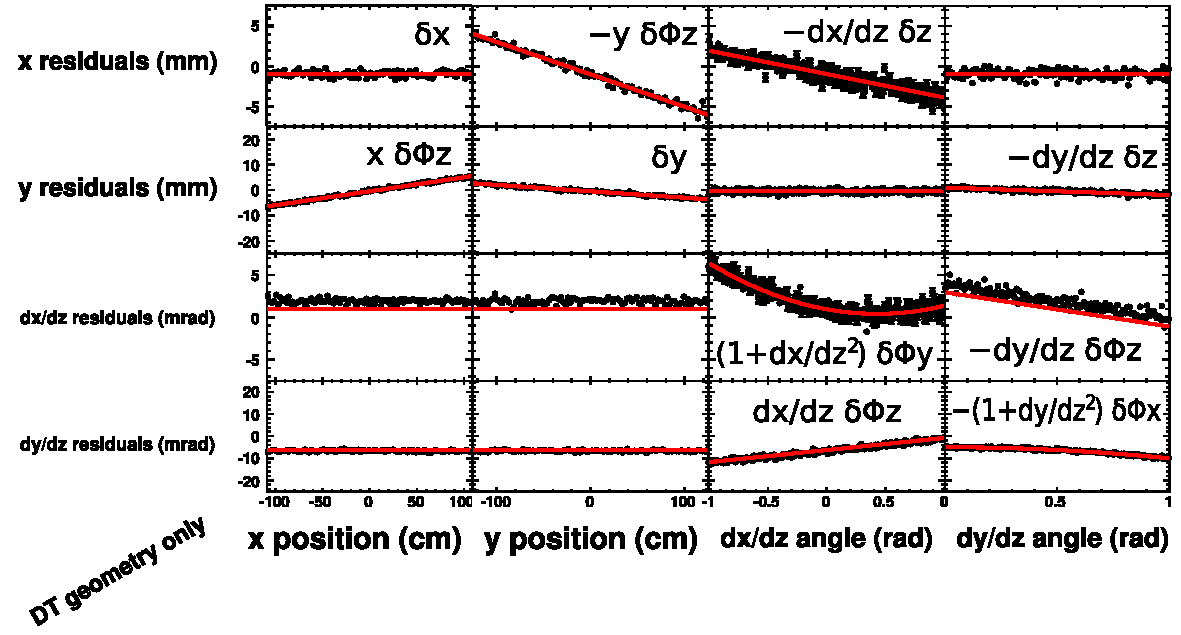
\includegraphics[width=\linewidth]{geometryonly_dt.pdf}
\end{frame}

\begin{frame}
\frametitle{Differential geometry of CSCs}

\begin{itemize}
\item We learned from beam-halo data that
\begin{itemize}
\item CSC wires are too granular for use in alignment
\item CSC strips fan from beamline, actually measure $r\phi$, not $x$
\end{itemize}

\item Two observables: $\Delta r\phi$ and $\Delta \frac{dr\phi}{dz}$
  with sensitivity to 6 DOF because of strip angle ($\delta_y$
  sensitivity is weak because it is suppressed by distance to beamline $R$)
\end{itemize}

\hfill 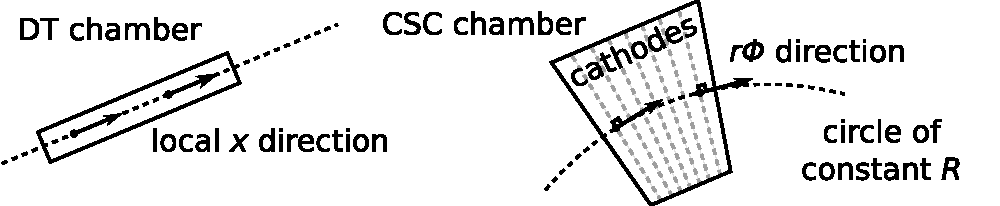
\includegraphics[width=0.65\linewidth]{strip_direction.pdf}

\vspace{-2 cm}
{\scriptsize 
\begin{multline*}
\renewcommand{\arraystretch}{3}
\left(\begin{array}{c}
{\Delta r\phi}^{\mbox{\tiny geom}} \\
{\Delta \dfrac{dr\phi}{dz}}^{\mbox{\tiny geom}} \\
\end{array}\right)
= \\
{\renewcommand{\arraystretch}{3}
\left(\begin{array}{c c c c c c}
1 & \left[ -\dfrac{x}{R} + 3\left(\dfrac{x}{R}\right)^3 \right] & -\dfrac{dx}{dz}  & -y \dfrac{dx}{dz} & x \dfrac{dx}{dz} & -y \\
0 & -\dfrac{dx}{dz}/(2R) & 0 & \left[ \dfrac{x}{R} - \dfrac{dx}{dz}\dfrac{dy}{dz} \right] & 1 + \left(\dfrac{dx}{dz}\right)^2 & -\dfrac{dy}{dz}
\end{array}\right)}
\renewcommand{\arraystretch}{1}
\left(\begin{array}{c}
\delta_x \\
\delta_y \\
\delta_z \\
\delta_{\phi_x} \\
\delta_{\phi_y} \\
\delta_{\phi_z}
\end{array}\right)
\label{eqn:cscmatrix}
\end{multline*}}
\end{frame}

\begin{frame}
\frametitle{Geometry-only MC}

\vspace{0.25 cm}
\begin{itemize}
\item Thoroughly tested this matrix, too \mbox{(and DT station 4's 5-DOF matrix)\hspace{-1 cm}}
\item Apparent gap between fit curve and data is a plotting artifact \\ (projecting a non-linear distribution onto one axis)
\item The fits converged on the true values of $\delta_x$, $\delta_y$, $\delta_z$, $\delta_{\phi_x}$, $\delta_{\phi_y}$, $\delta_{\phi_z}$
\end{itemize}

\vspace{0.5 cm}
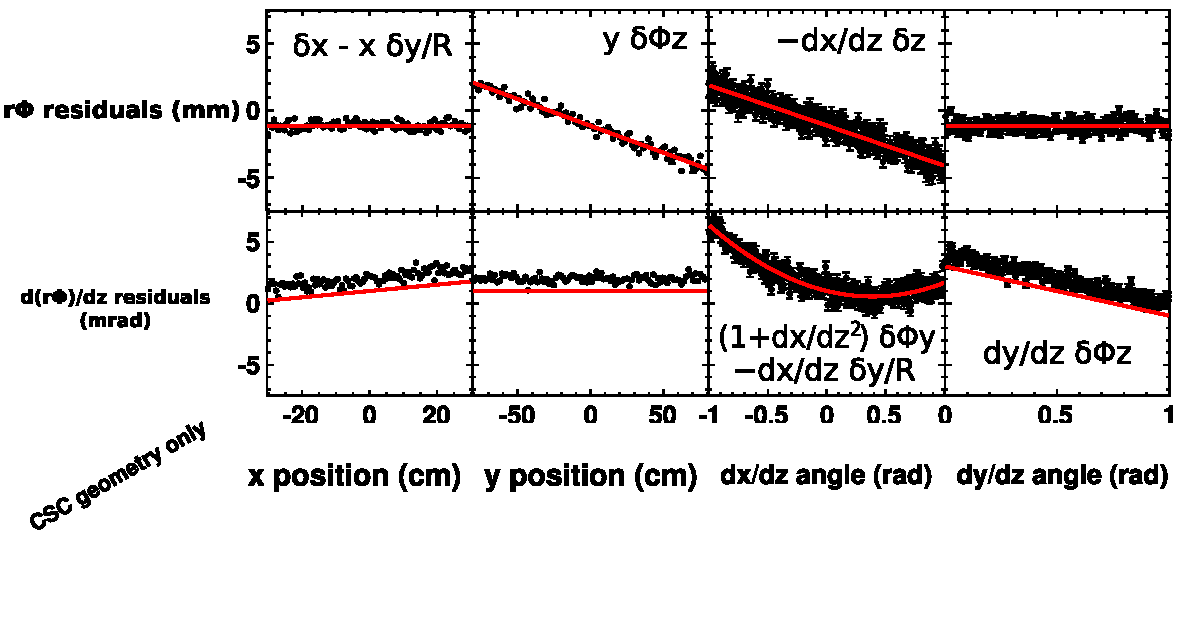
\includegraphics[width=\linewidth]{geometryonly_csc.pdf}
\end{frame}

\begin{frame}
\frametitle{Full MC studies}

\begin{columns}
\column{0.35\linewidth}

\vspace{0.3 cm}
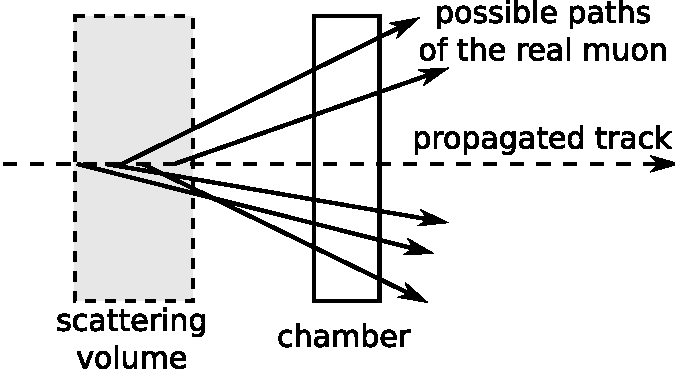
\includegraphics[width=1.15\linewidth]{sawtooth_diagram.pdf}

\vspace{-0.7 cm}
\mbox{ }

\column{0.7\linewidth}
\begin{itemize}
\item Full MC includes known measurement effects
\item Correlation between $y$ and $\frac{dy}{dz}$ \mbox{(fig on left)\hspace{-0.5 cm}} introduces plotting artifacts (``echo'')
\item Real structure in GEANT but not track reconstruction
\end{itemize}
\end{columns}

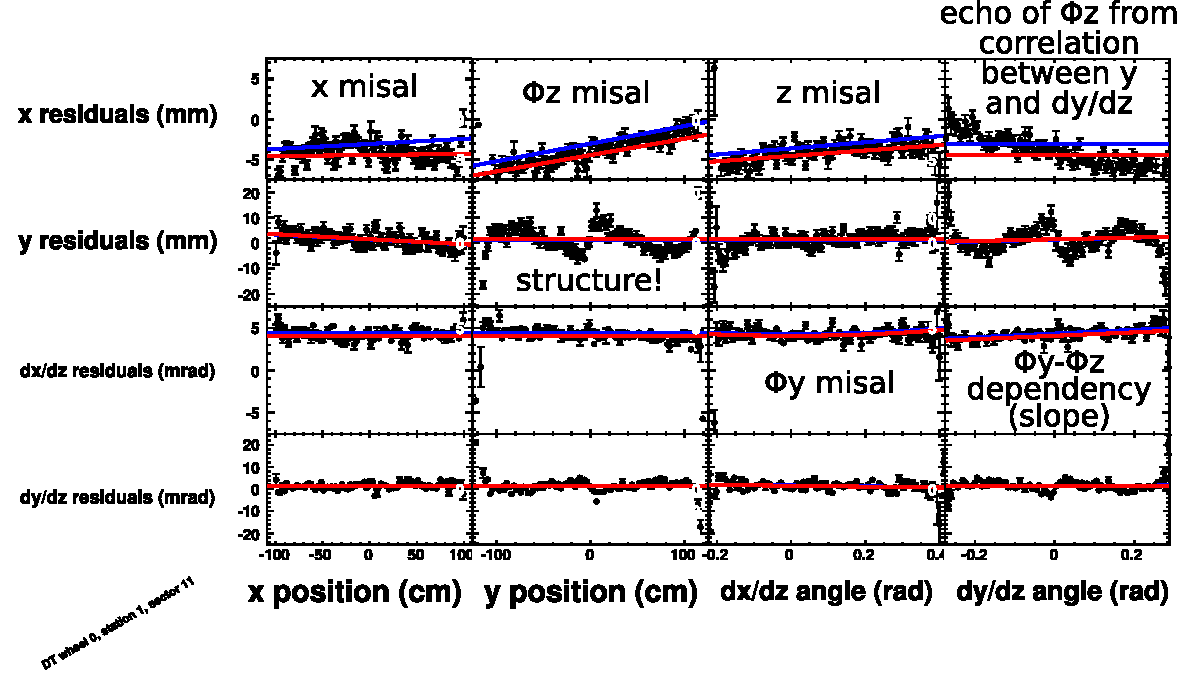
\includegraphics[width=\linewidth]{mcfit_misal_and_nongeom.pdf}
\end{frame}

\begin{frame}
\frametitle{Same chamber, aligned}
\begin{itemize}
\item ``Echo'' disappears because $\phi_z$ was corrected
\item Internal DT structure is not alignable with rigid body parameters
\item \textcolor{red}{Red} and \textcolor{blue}{blue} are $\mu^+$ and $\mu^-$ from two-bin method
\begin{itemize}
\item corrects for $dE/dx$ errors in addition to $\vec{B}(\vec{x})$; \\
  the propagator uses a different material description \mbox{than GEANT\hspace{-1 cm}}
\end{itemize}
\end{itemize}

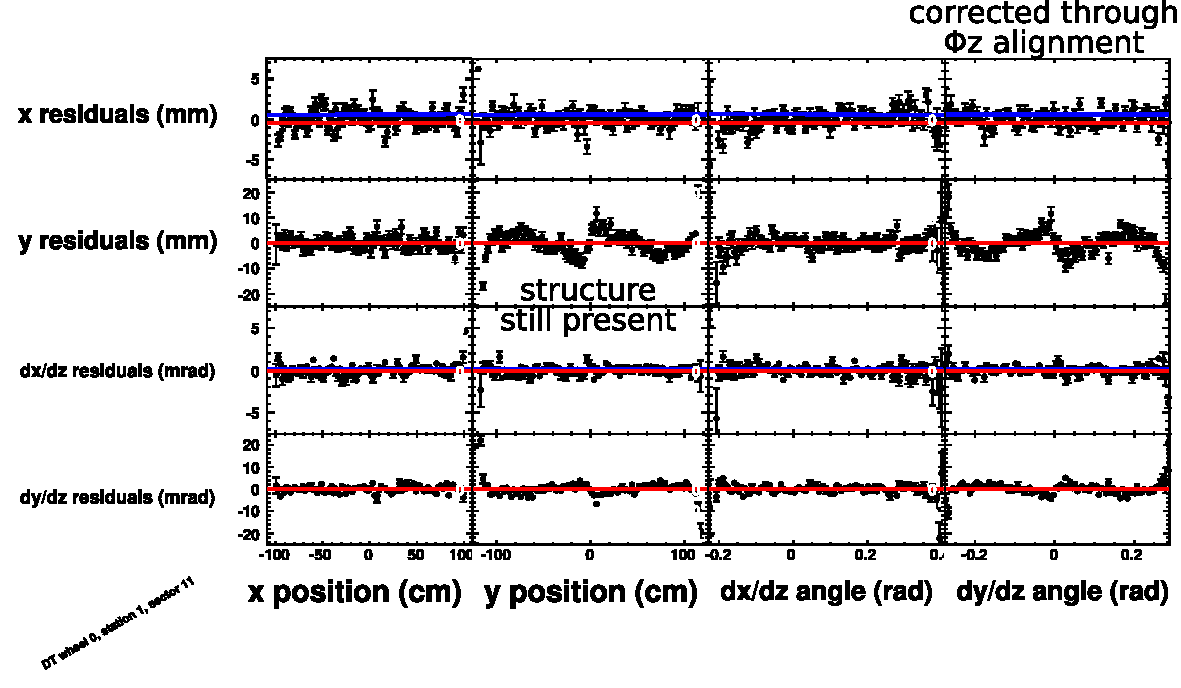
\includegraphics[width=\linewidth]{mcfit_misal_and_nongeom_aligned.pdf}
\end{frame}

\begin{frame}
\frametitle{Highly descriptive fit function}

\begin{itemize}
\item Non-Gaussian tails accounted for (\textcolor{red}{red} is fit to
  $\mu^+$, shown in black, \textcolor{blue}{blue} is for $\mu^-$, not
  shown)
\item Expected $x$, $\frac{dx}{dz}$ and $y$, $\frac{dy}{dz}$
  correlations are included (semi-major axis of error ellipse shown as
  a line on the $\mu^+$ scatter plot)
\item This chamber is in the corner of the barrel (hardest to satisfy)
\end{itemize}

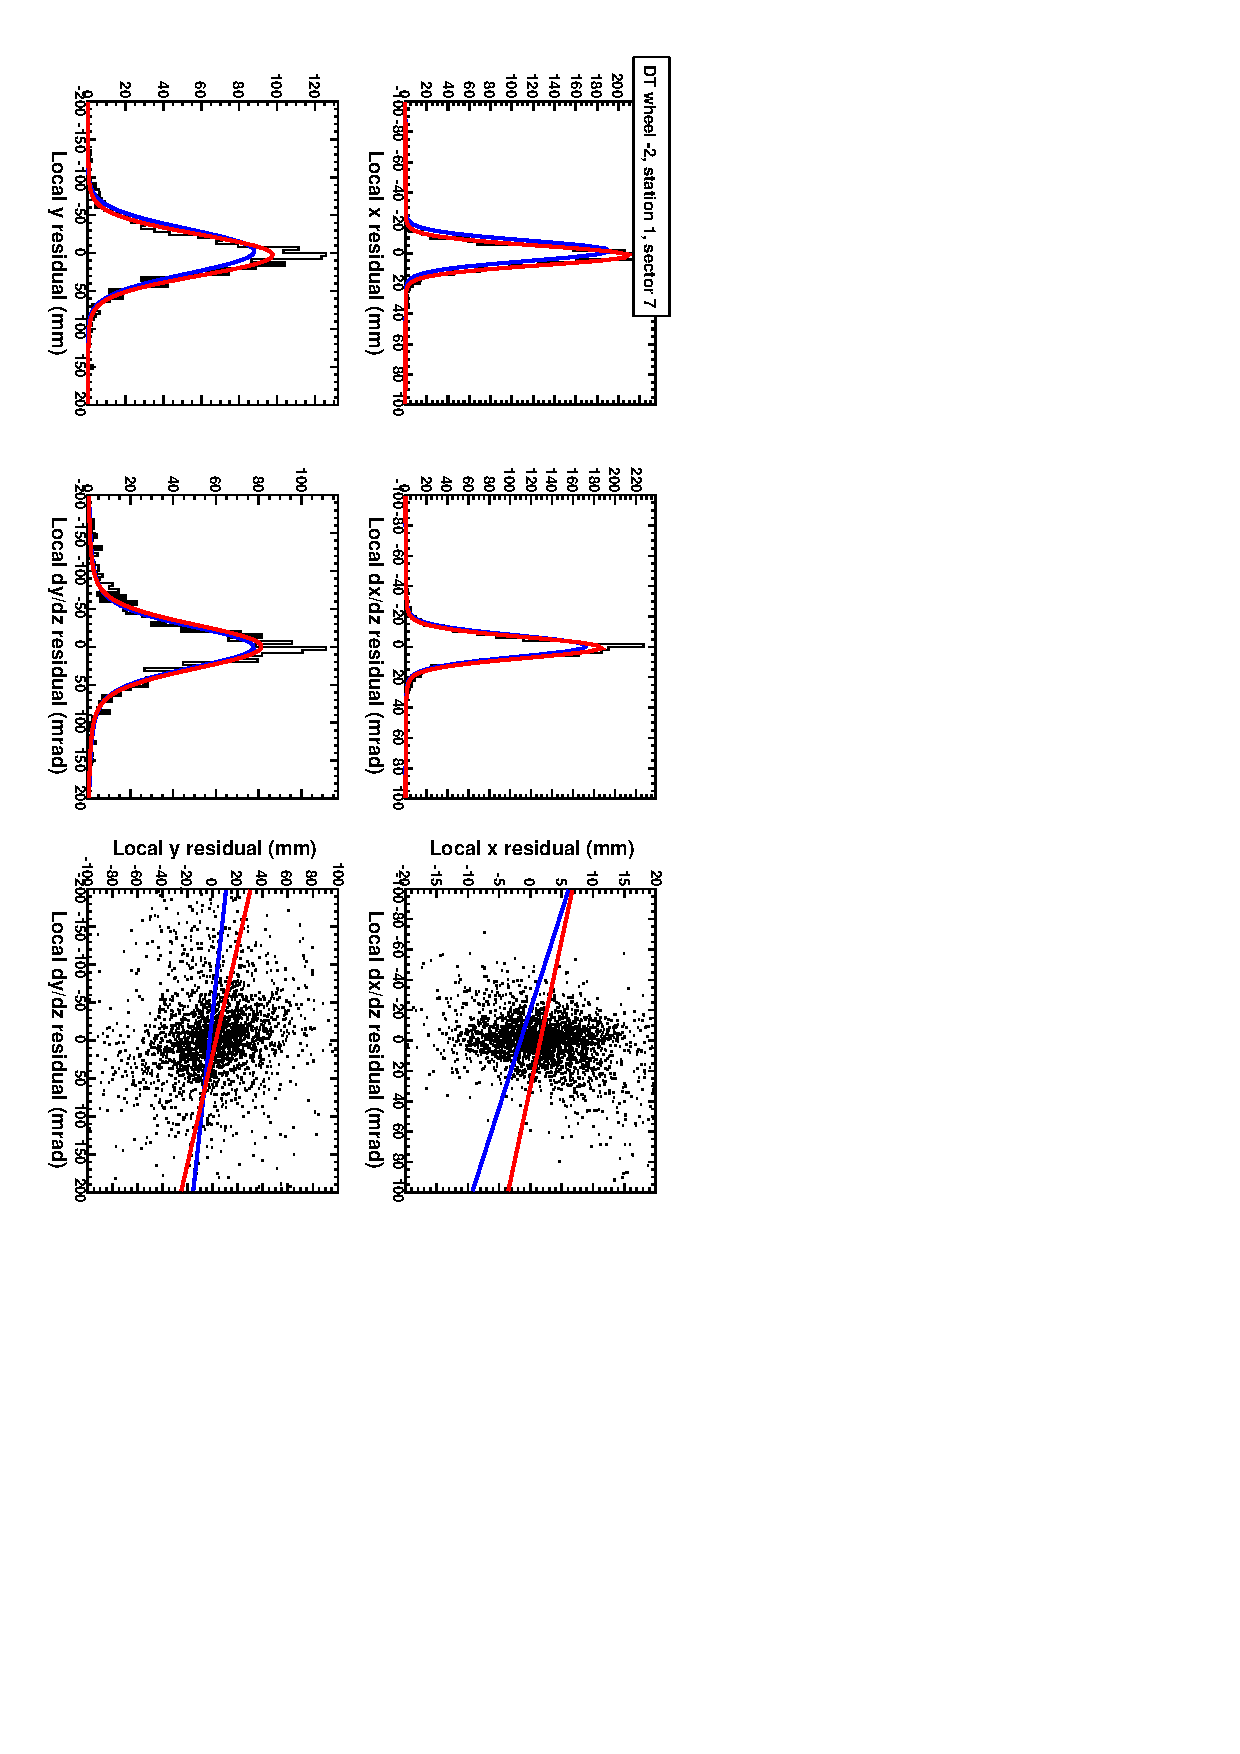
\includegraphics[height=\linewidth, angle=90]{mcfit_extreme_corner2.pdf}
\end{frame}

\begin{frame}
\frametitle{MC accuracy}

\begin{itemize}
\item Workflow applied to 50~pb$^{-1}$ inclusive $\mu$ MC as though it were data
\item 400~$\mu$m $r\phi$ (local $\delta_x$) resolution in {\it all} stations and endcap
\item Radial alignment (local $\delta_z$) biased by an effect described on \mbox{next page\hspace{-1 cm}}
\item Wrong radius implies wrong global $z$ (local $\delta_y$) except in wheel~0
\end{itemize}

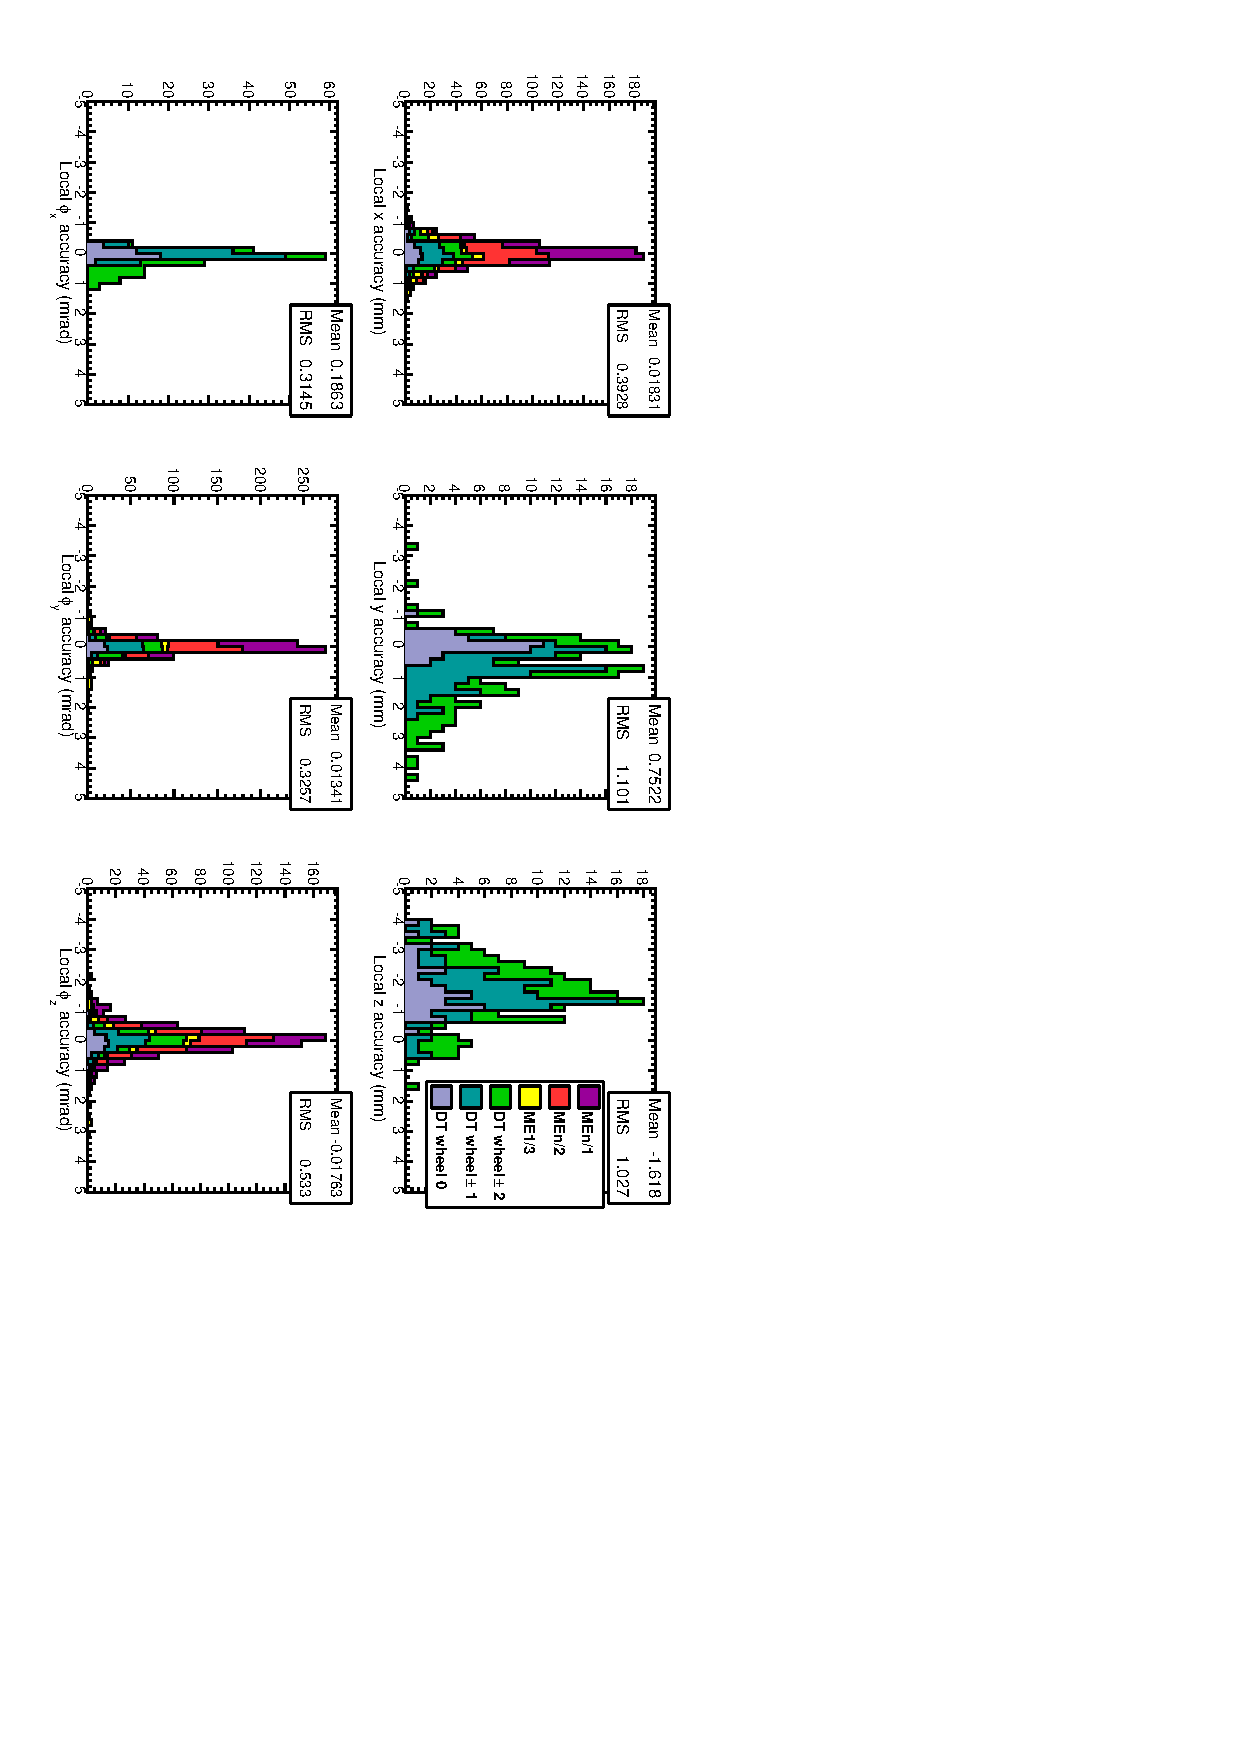
\includegraphics[height=\linewidth, angle=90]{mc_accuracy.pdf}
\end{frame}

\begin{frame}
\frametitle{Why local $\delta_z$ is biased}

\begin{center}
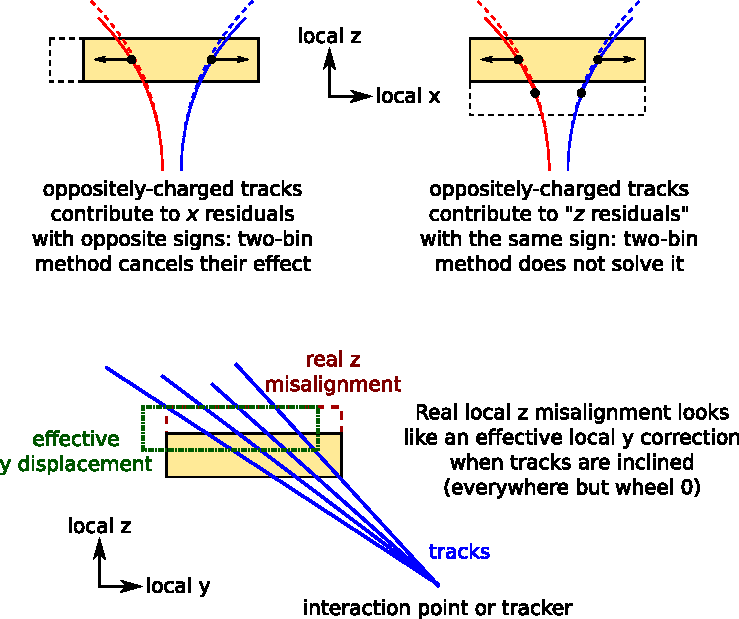
\includegraphics[width=0.9\linewidth]{explanation_of_z.pdf}
\end{center}
\end{frame}

\begin{frame}
\frametitle{Accuracy of quoted uncertainties}

\begin{itemize}
\item Uncertainties from Minuit's HESSE are 1.7--2.5 times too small
\item Minuit's strategy=2 and MINOS yield differences in quoted
  uncertainties on this scale, but zero differences in the central value
\begin{itemize}
\item both algorithms are also slow to compute
\end{itemize}
\end{itemize}

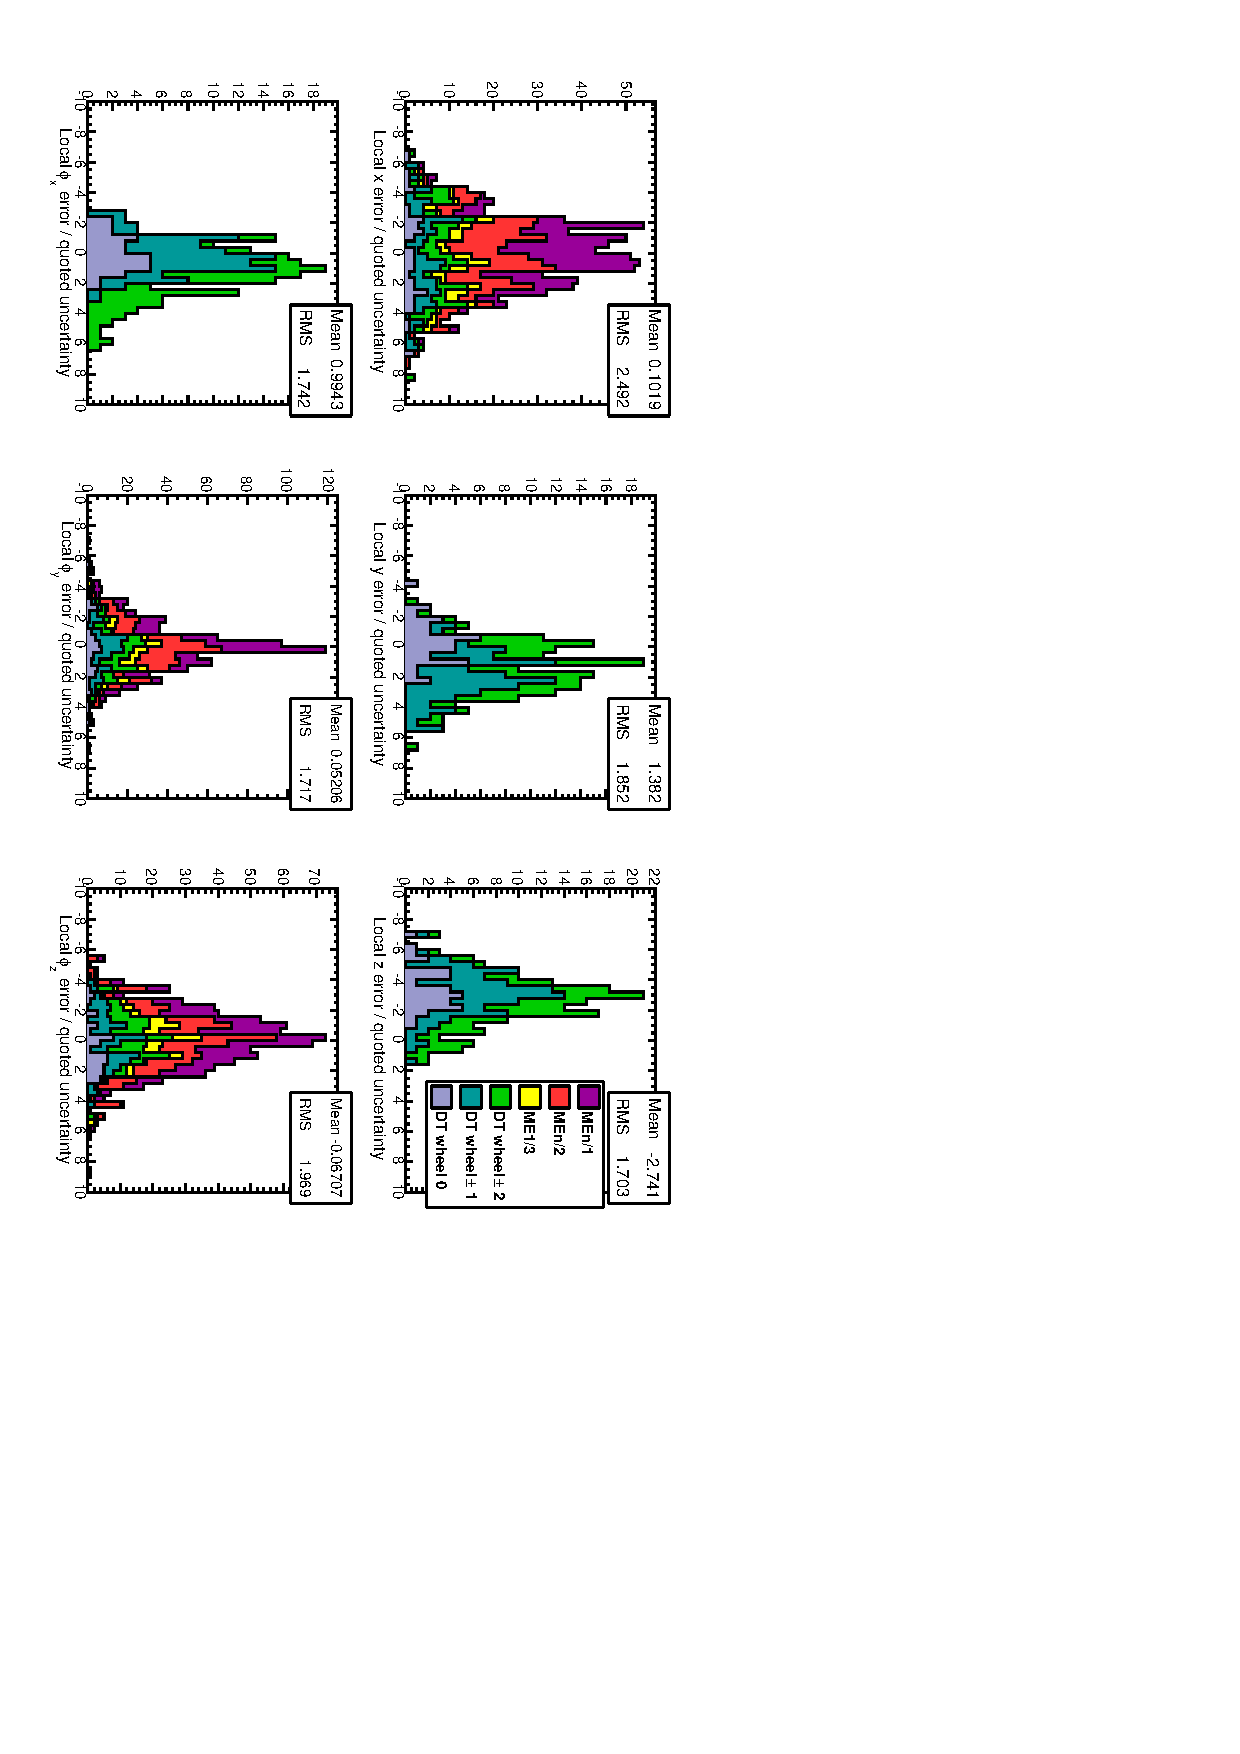
\includegraphics[height=\linewidth, angle=90]{mc_accuracy_of_uncertainties.pdf}
\end{frame}

\begin{frame}
\frametitle{Convergence}

\begin{itemize}
\item Most parameters converge in 1 iteration (purple to yellow)
\item $\delta_x$ requires two iterations to reach final accuracy (green)
\item $\Delta x$ residuals are the most affected by $dE/dx$ errors,
  largest $\dfrac{\delta_x(\mu^+) - \delta_x(\mu^-)}{2}$ (two-bin correction is applied outside of fitter)
\end{itemize}

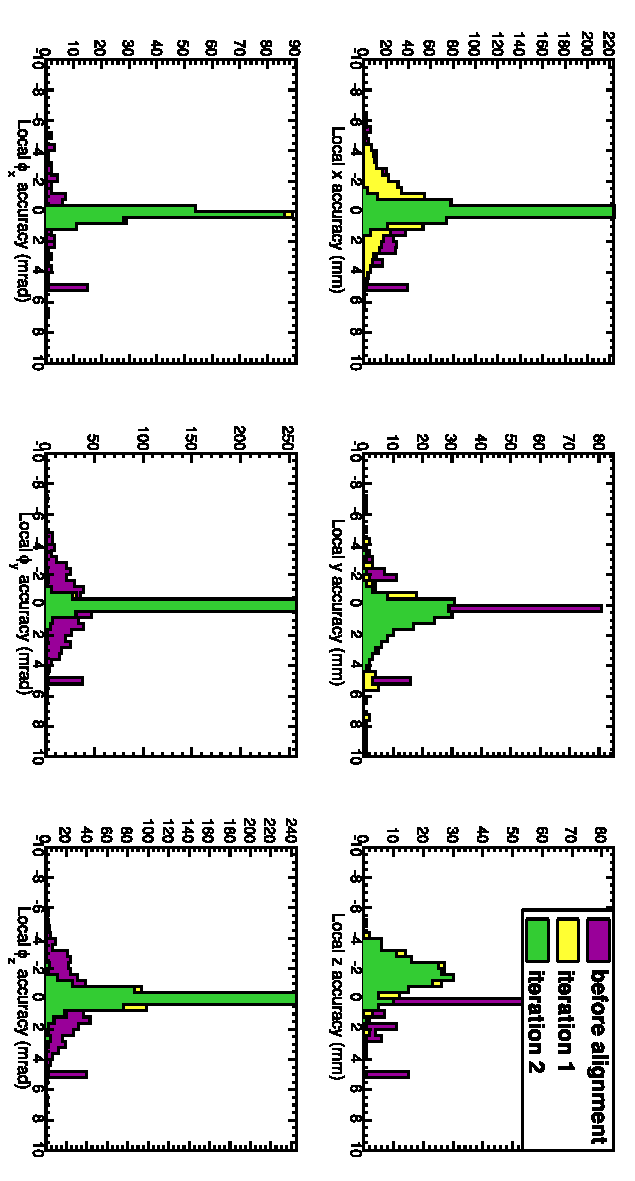
\includegraphics[height=\linewidth, angle=90]{mc_convergence.pdf}
\end{frame}

\begin{frame}
\frametitle{Alignment of data}

\begin{itemize}\setlength{\itemsep}{0.2 cm}
\item From this point onward, all plots will show CRAFT data
\item First we will consider a 6-DOF alignment of DTs
\item Then we will restrict local $\delta_z$ and some $\delta_y$ to
  obtain a production-quality alignment for TrackerPointing and SuperPointing re-processing
\item Then we will use the same framework to investigate CSC misalignments
\end{itemize}
\end{frame}

\begin{frame}
\frametitle{A typical DT (after alignment)}

\vspace{0.25 cm}
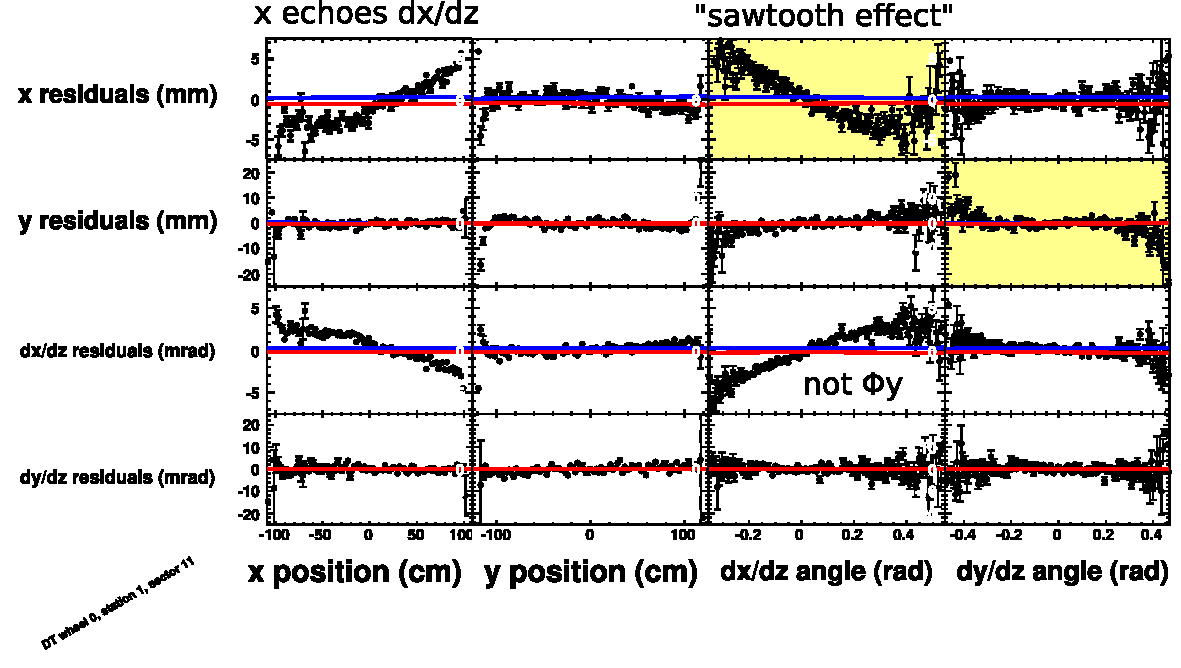
\includegraphics[width=\linewidth]{datafit_sawtooth.pdf}

\vspace{-0.5 cm}
\begin{itemize}
\item Known ``sawtooth effect'' is linearly independent of
  $\delta_z$ (which affects both yellow plots) and
  $\delta_{\phi_y}$ (which is symmetric in $\frac{dx}{dz}$)
\item All correlations seen here agree with the single-chamber study
\item All of these arguments were made before, but never in one plot
\end{itemize}
\end{frame}

\begin{frame}
\frametitle{Bell-curves for the same chamber}

\begin{itemize}
\item Reminder: \textcolor{red}{red} curves fit black $\mu^+$ data, \\ \textcolor{white}{Reminder:} \textcolor{blue}{blue} curves fit $\mu^-$ data, not shown
\item Lines are the semi-major axes of error ellipses
% \item Charge asymmetry can be large (like 5:1) for some chambers, depending on location; very important to weight them equally
\end{itemize}

\vfill
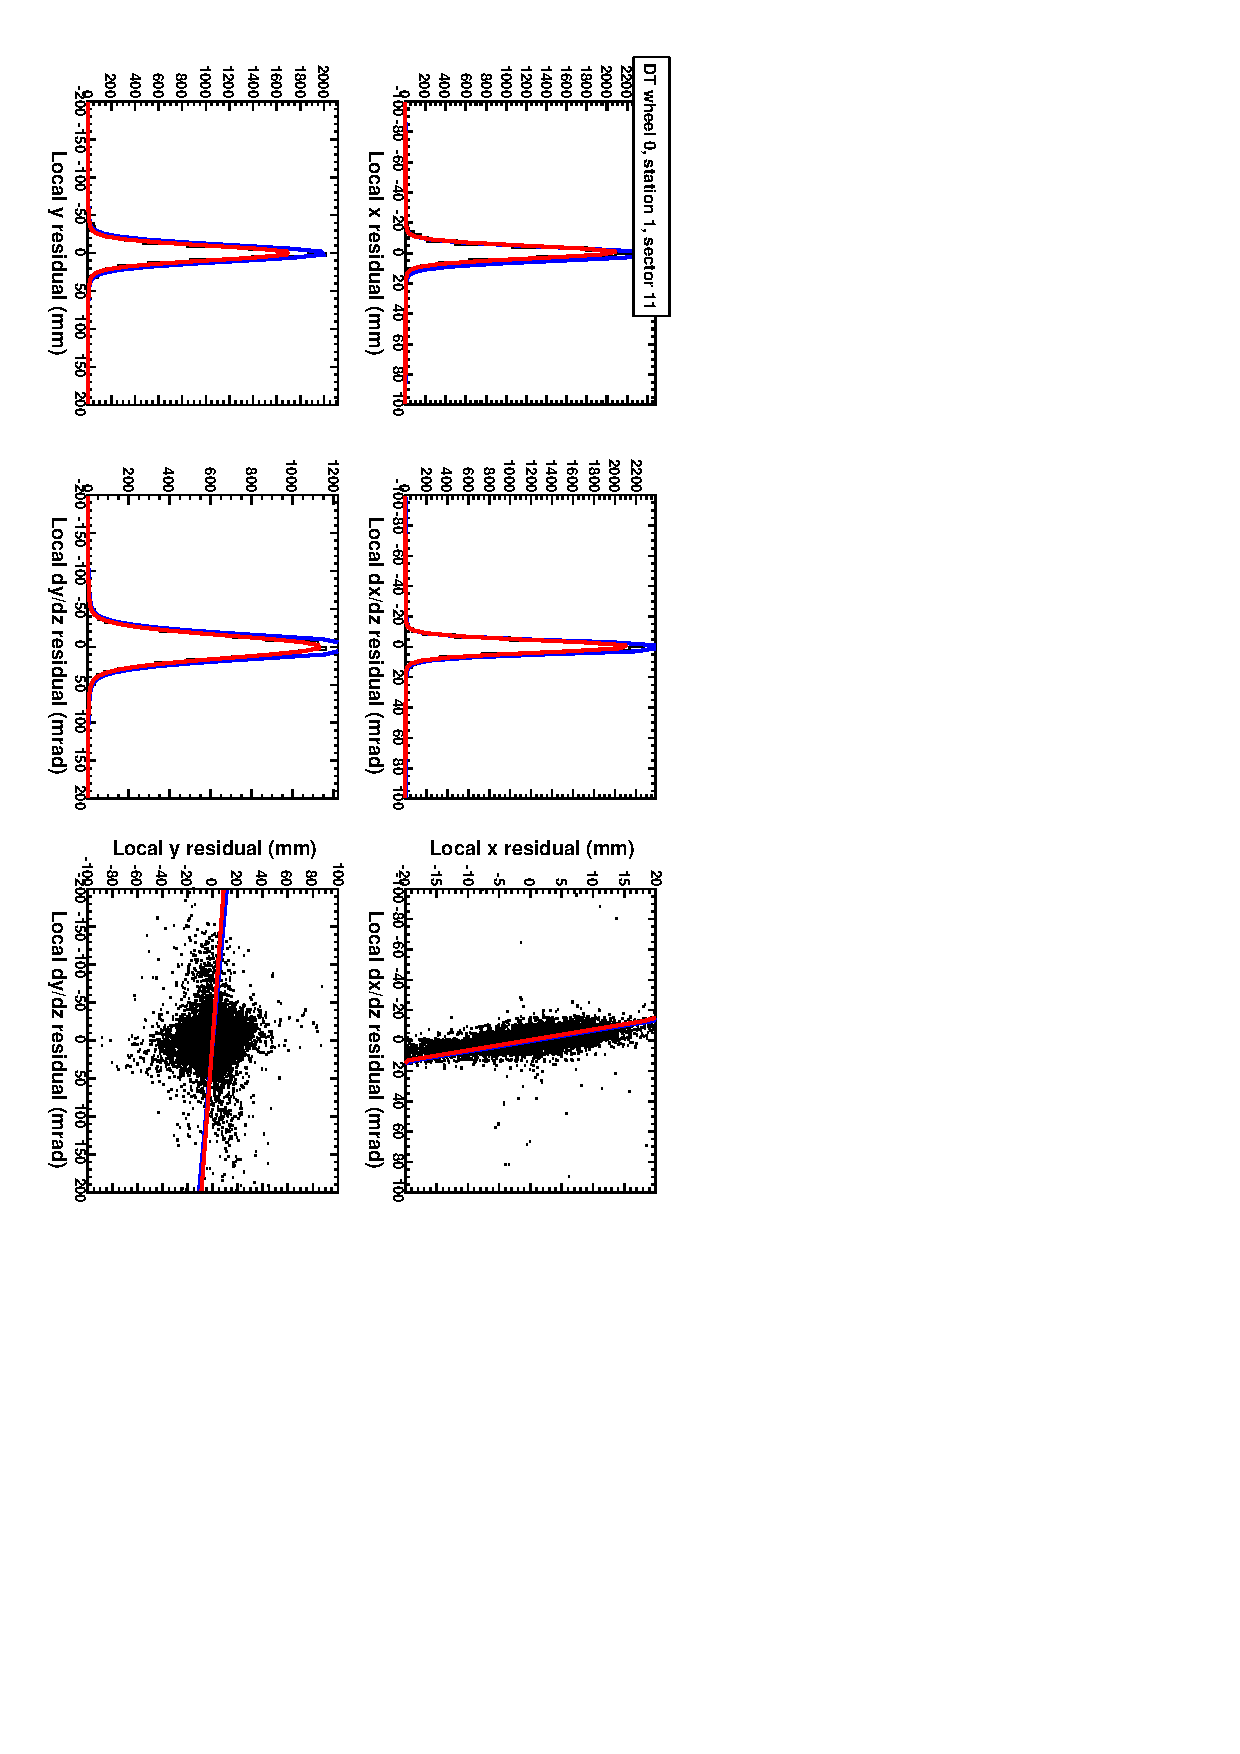
\includegraphics[height=\linewidth, angle=90]{datafit_sawtooth2.pdf}
\end{frame}

\begin{frame}
\frametitle{Extreme corner of barrel}

\begin{itemize}
\item Another example, this one is from wheel~2, station~1 where non-Gaussianess of residuals is most extreme
\item Note \textcolor{red}{$\mu^+$}/\textcolor{blue}{$\mu^-$}
  splitting in $\Delta y$ residuals, rather than $\Delta x$: this is
  also the only part of the barrel with a radial $\vec{B}(\vec{x})$
\end{itemize}

\vfill
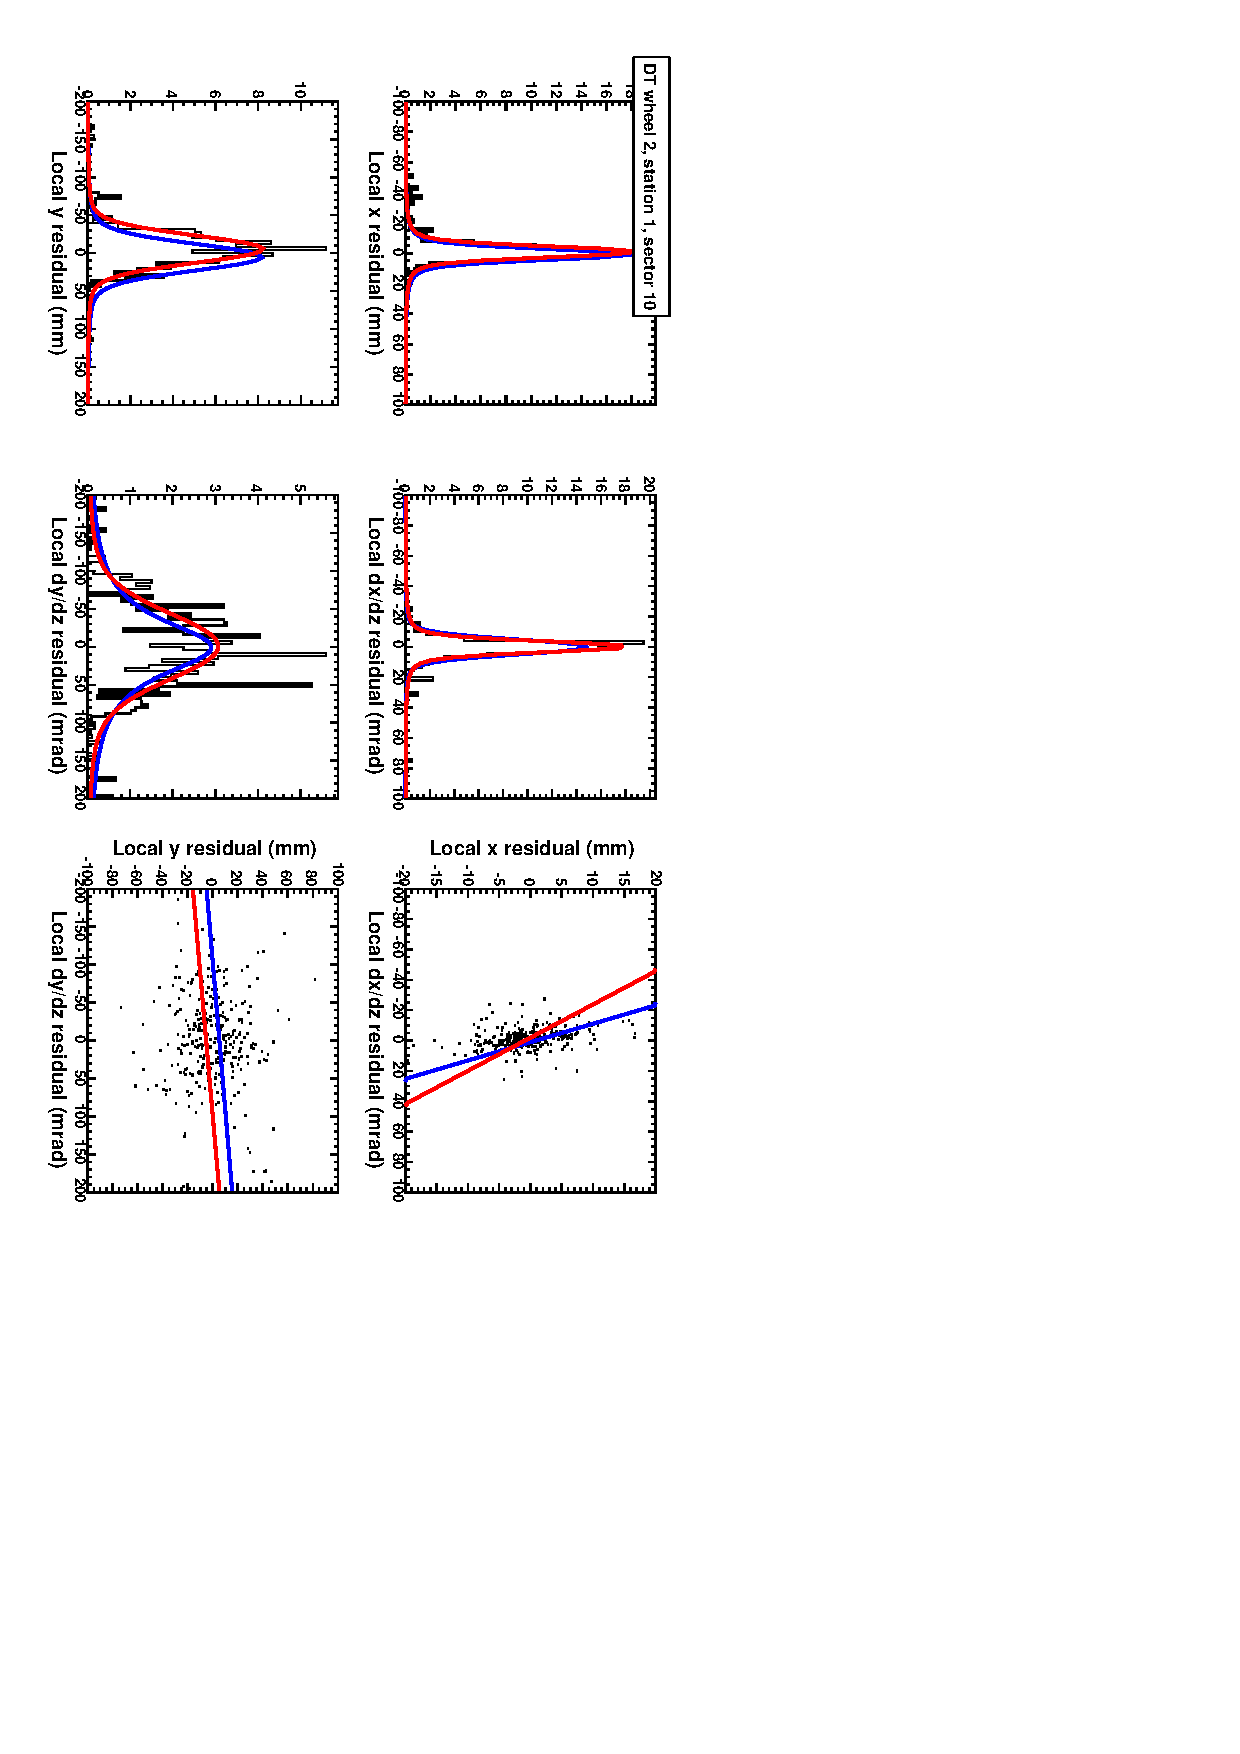
\includegraphics[height=\linewidth, angle=90]{datafit_extreme_corner2.pdf}
\end{frame}

\begin{frame}
\frametitle{Station~4 structure}

\vspace{0.5 cm}
\begin{columns}
\column{0.8\linewidth}
\begin{itemize}
\item Some station~4 chambers show the sawtooth effect
\item But sectors 4 and 13 also have a sharp step laterally down the center ($x=0$)
\item Gap between \textcolor{red}{$\mu^+$} and \textcolor{blue}{$\mu^-$} is due to $\vec{B}(\vec{x})$ errors
\end{itemize}

\column{0.25\linewidth}
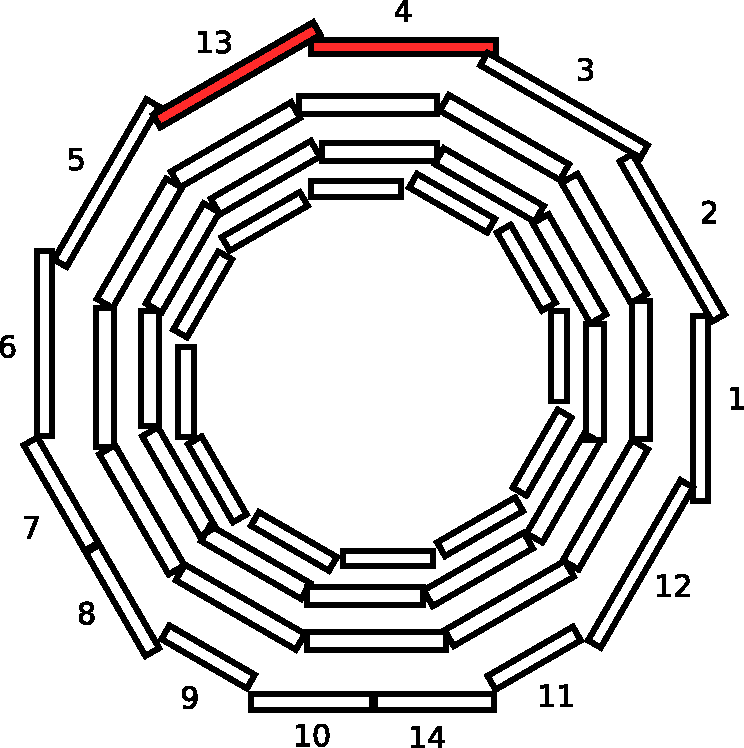
\includegraphics[width=\linewidth]{location_of_04_13.pdf}
\end{columns}

\vspace{0.25 cm}
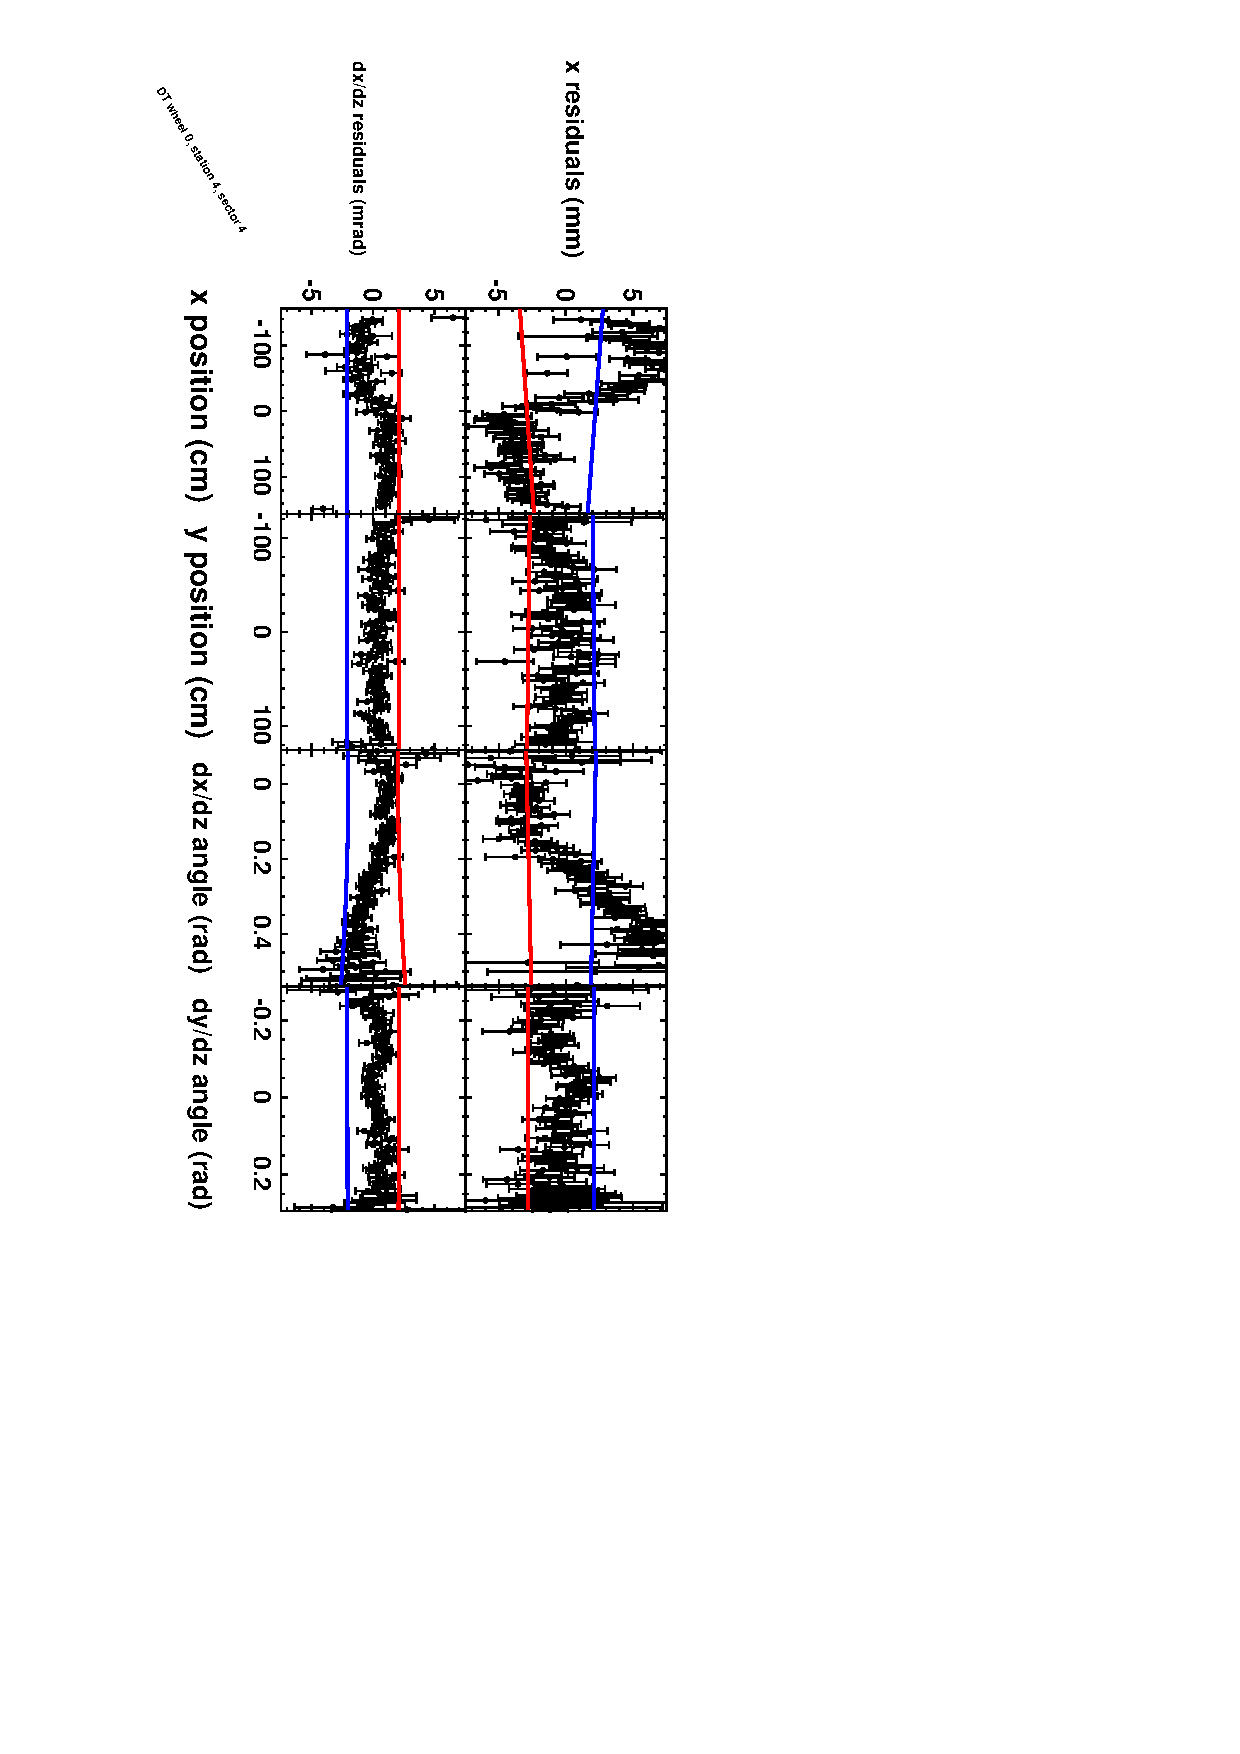
\includegraphics[height=\linewidth, angle=90]{datafit_st4sec_04_13.pdf}
\end{frame}

\begin{frame}
\frametitle{But some are perfect}

\begin{itemize}
\item The degree of sawtooth varies from chamber to chamber
\end{itemize}

\vfill
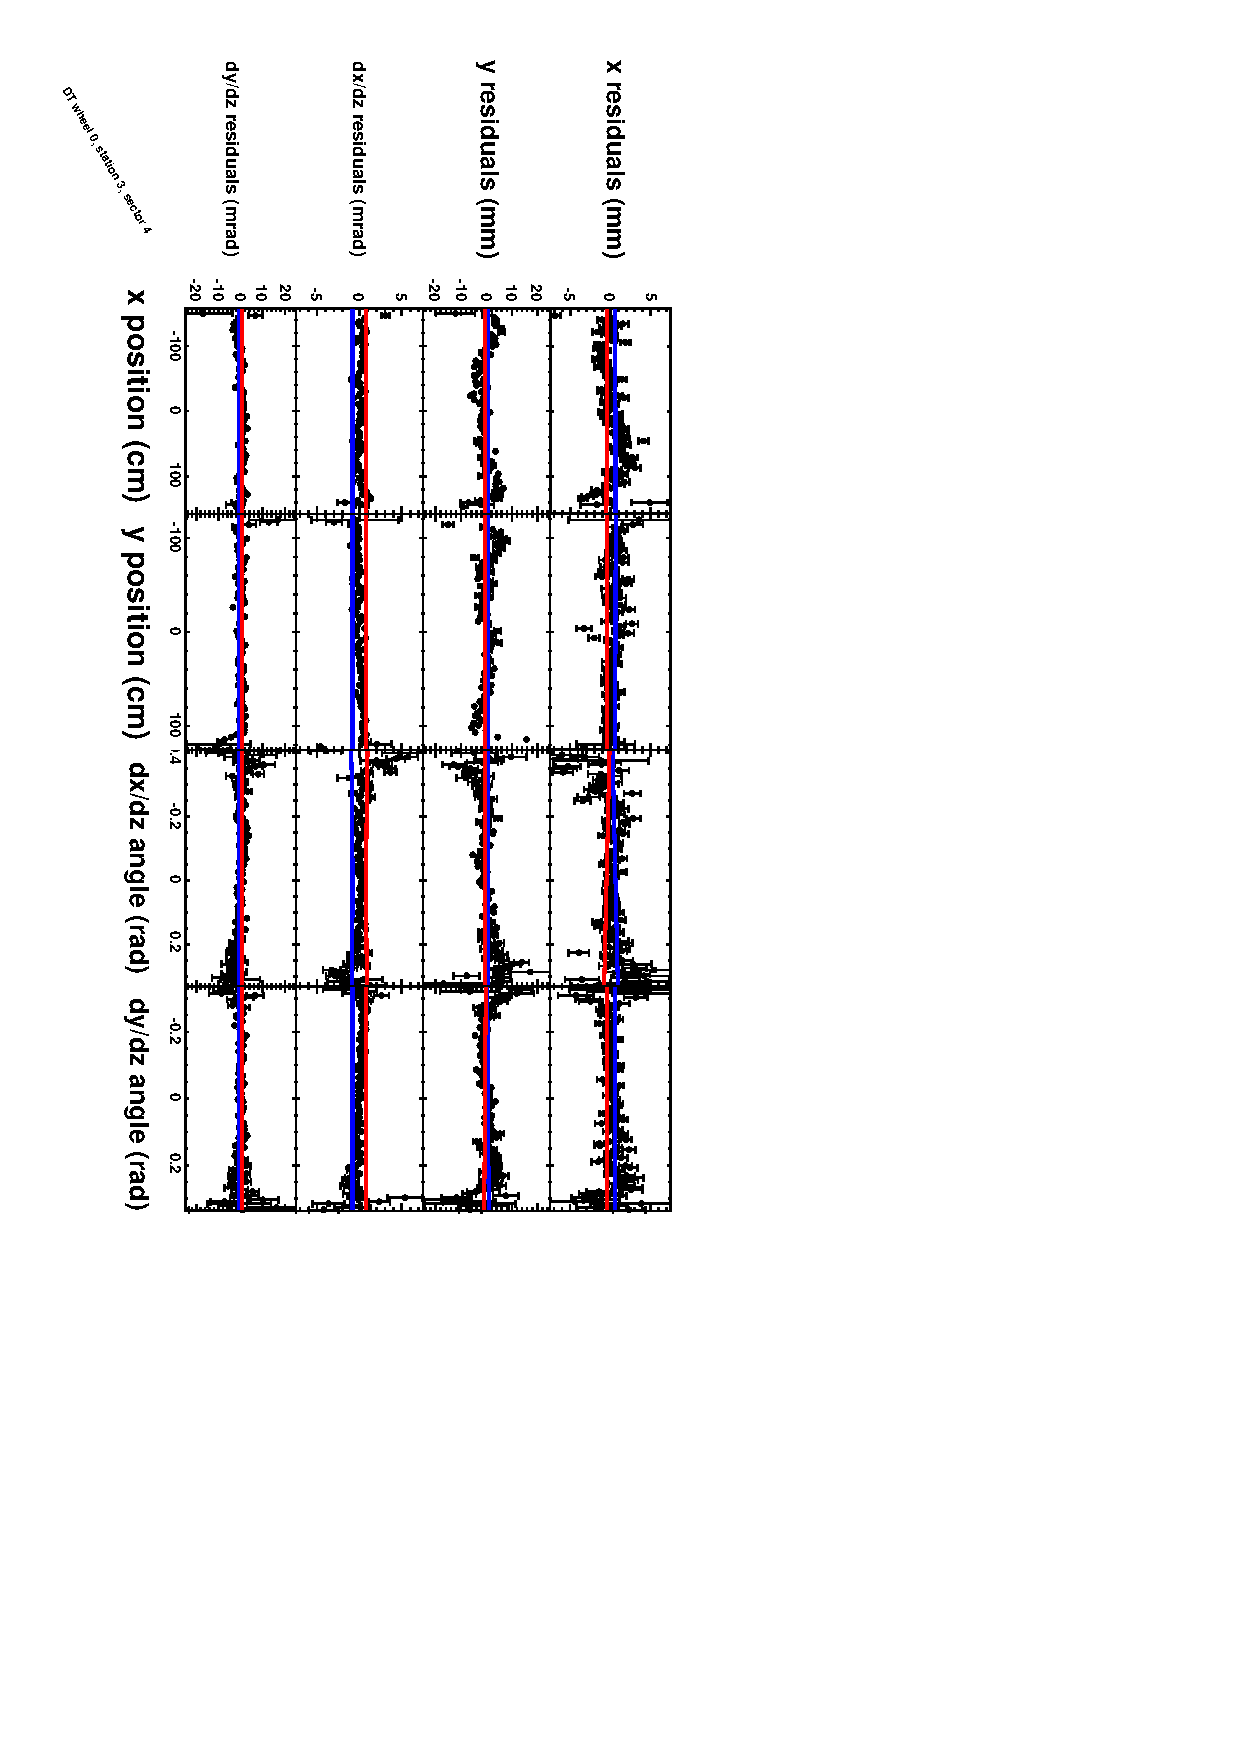
\includegraphics[height=\linewidth, angle=90]{datafit_some_are_perfect.pdf}
\end{frame}

\begin{frame}
\frametitle{Which chambers were aligned}

\begin{itemize}
\item Pattern of convergence and resolution follow cosmic ray statistics
\item ``Convergence'' = no change in parameters after 4 iterations
  bigger than 0.1~mm, 0.1~mrad
\end{itemize}

\vfill
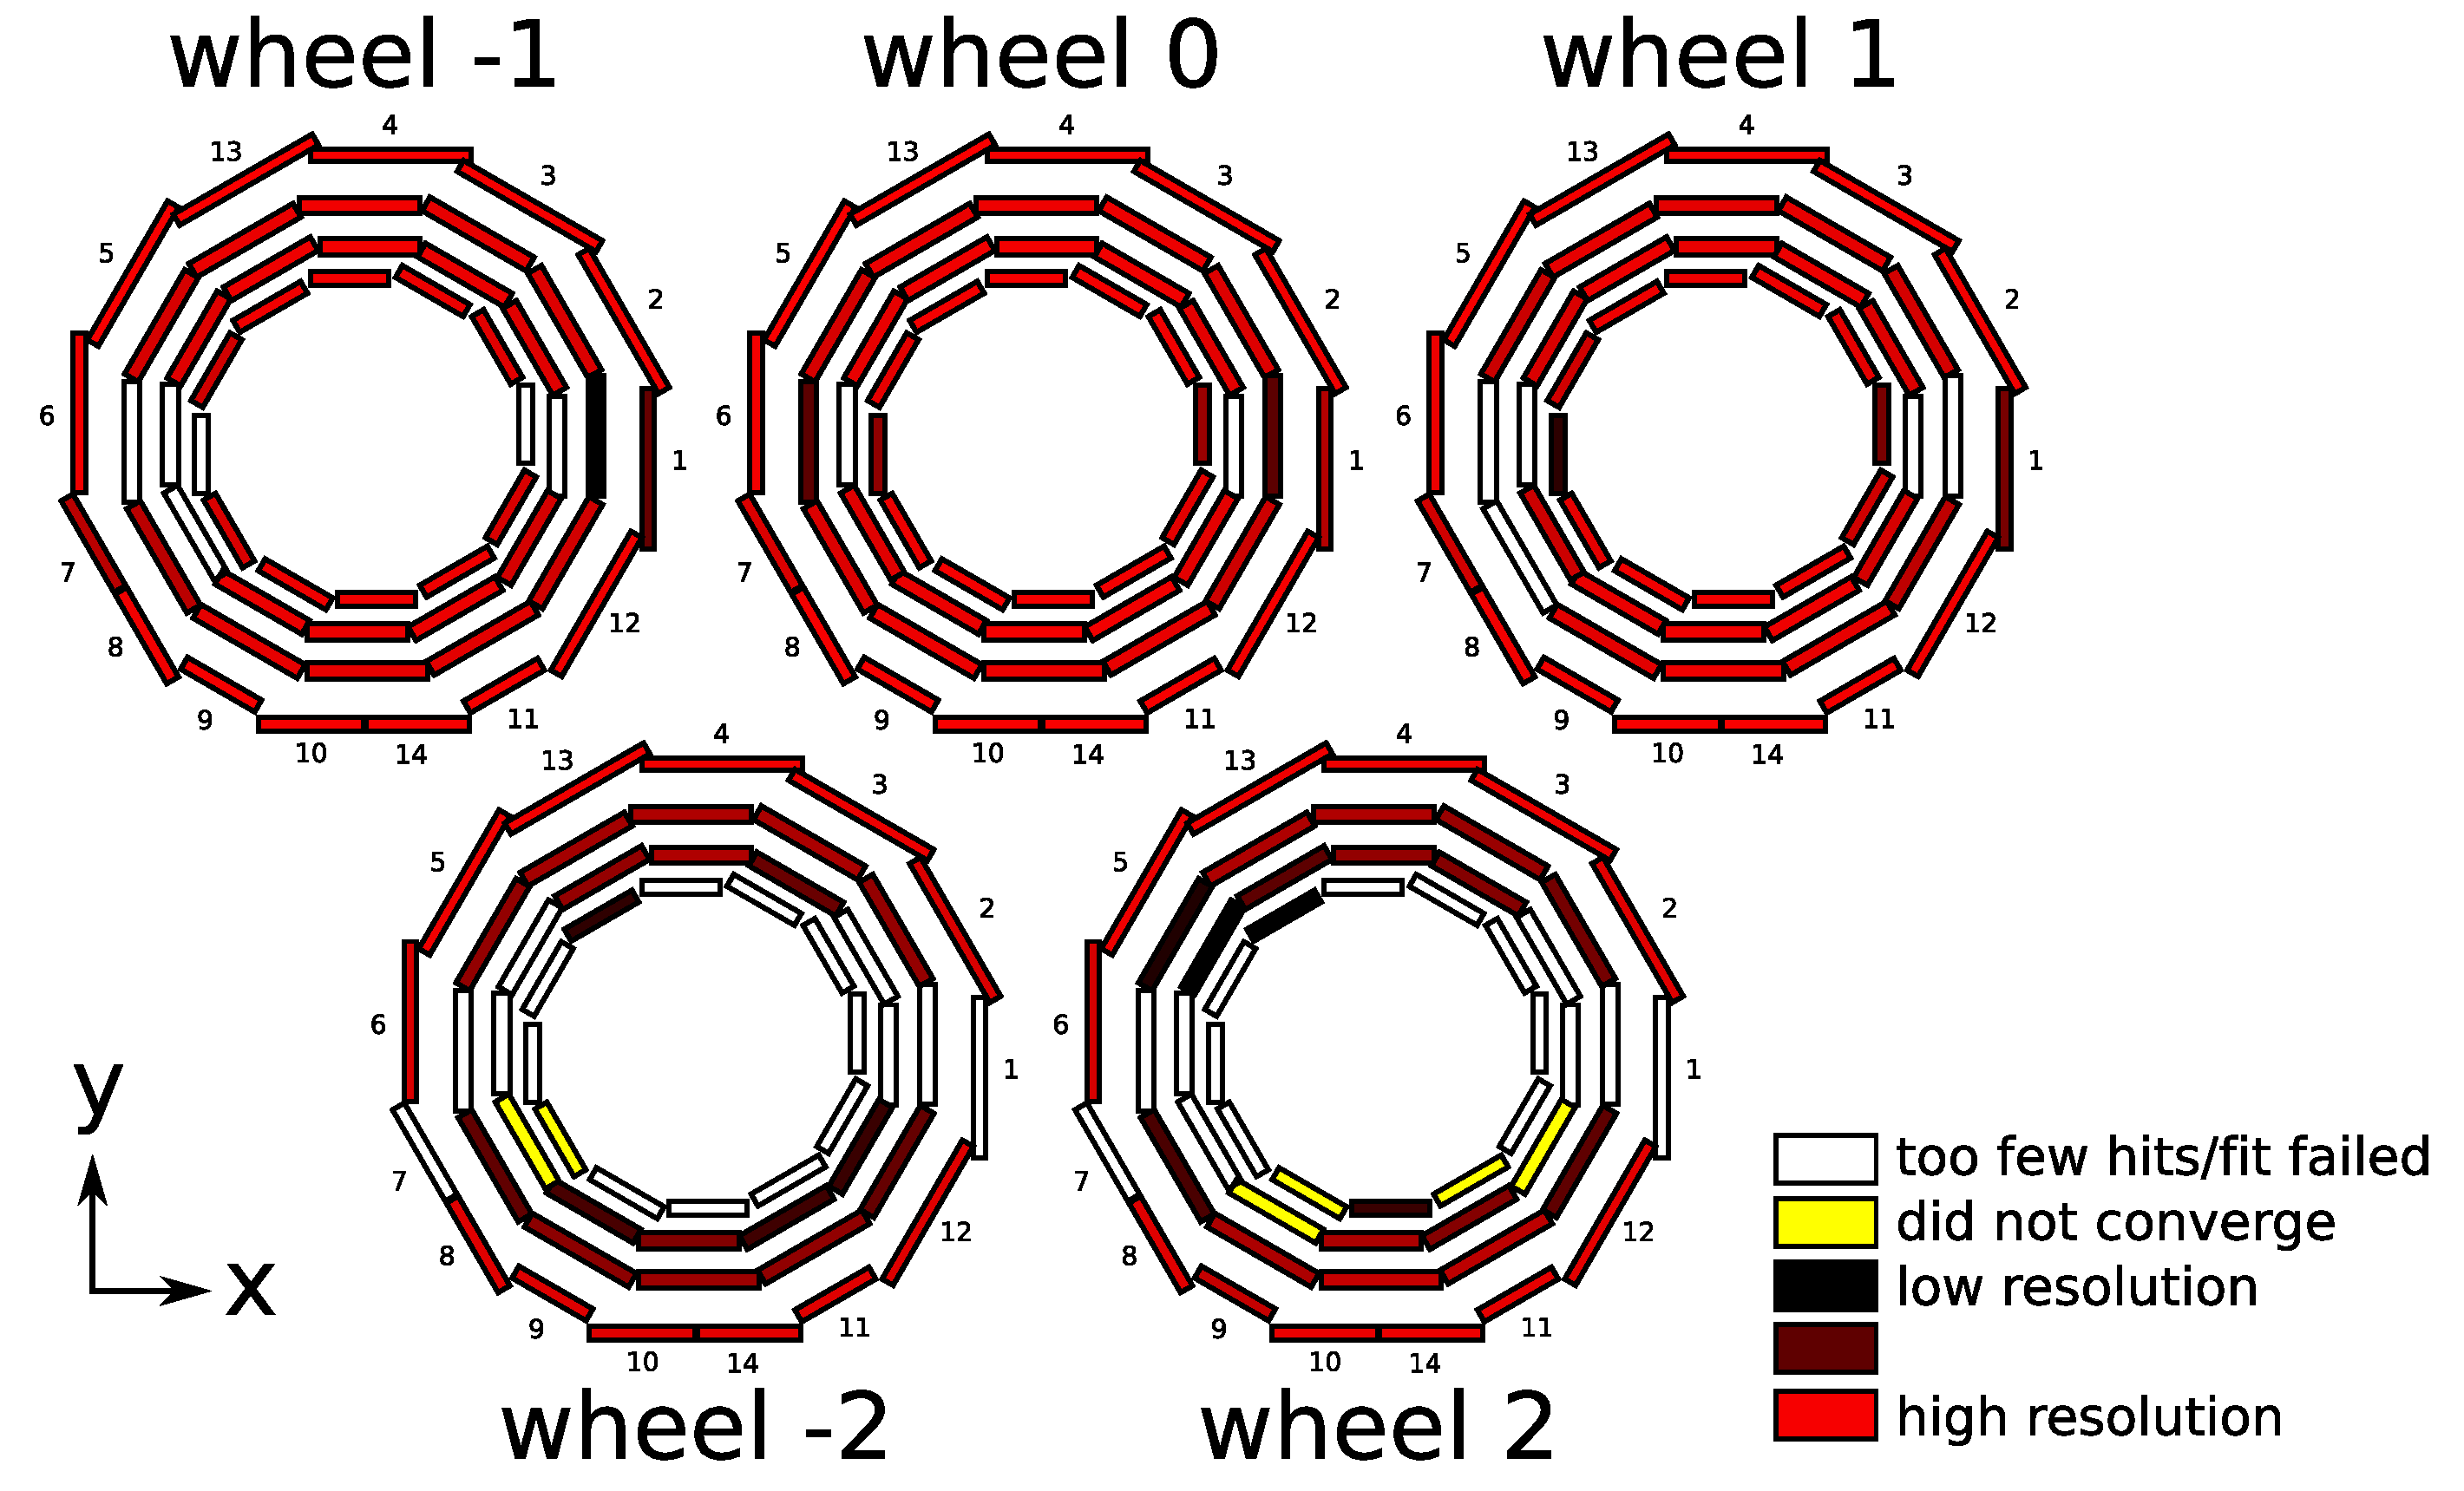
\includegraphics[width=\linewidth]{data_convergence.pdf}
\end{frame}

\begin{frame}
\frametitle{Alignment corrections}

\begin{itemize}
\item Changes in parameters, with respect to the previous geometry
\item Wide spread in local $\delta_z$, and hence $\delta_y$ differences (will be fixed later)
\item No evidence for a coherent rotation of any wheel, though individual chambers shifted by local $\delta_x = 2$~mm ($\delta_{\mbox{\scriptsize ``$\phi$''}} = 0.5$~mrad)
\item Note the large $\delta_{\phi_x}$, $\delta_{\phi_y}$ corrections (new with this alignment)
\end{itemize}

\vfill
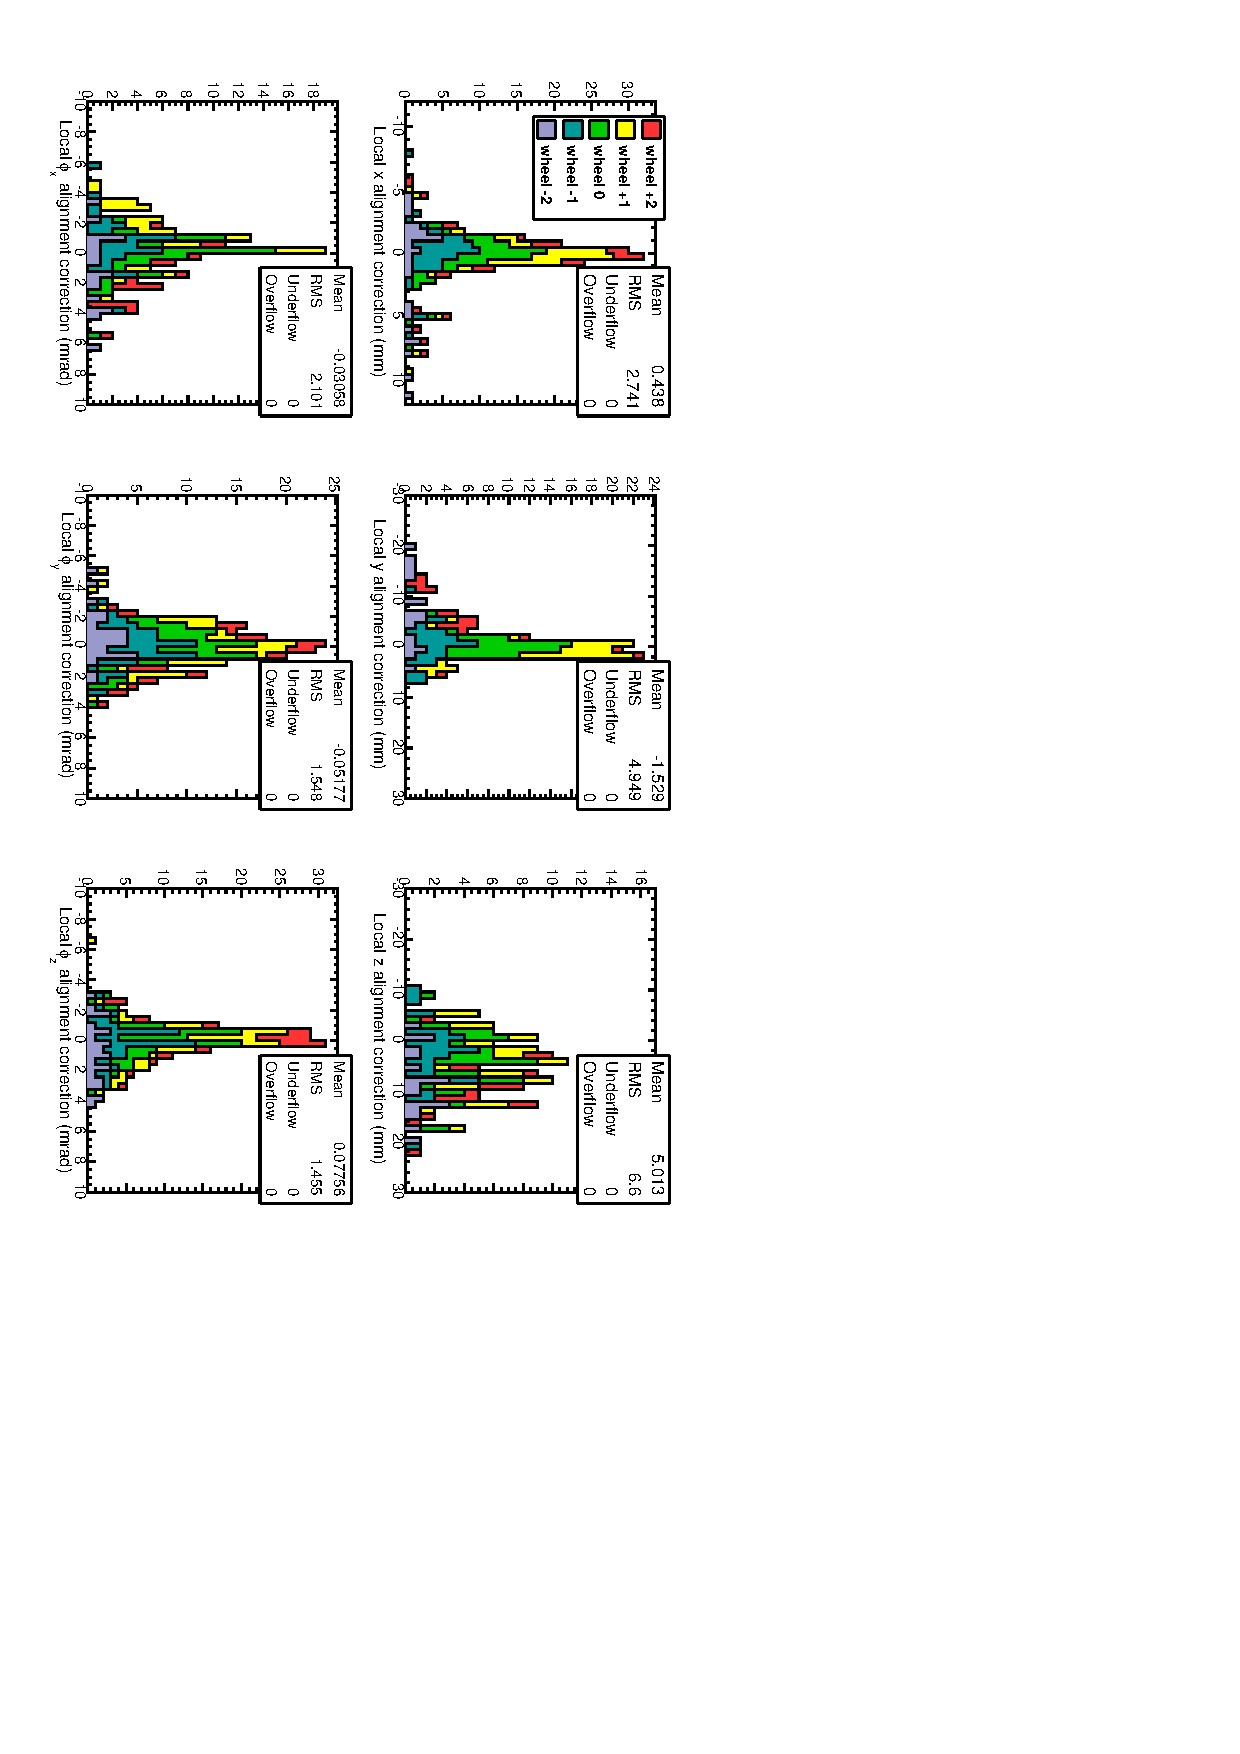
\includegraphics[height=0.95\linewidth, angle=90]{data_alignment_corrections.pdf}
\end{frame}

\begin{frame}
\frametitle{Quoted uncertainties}

\begin{itemize}
\item Most are below 0.3~mm, 0.3~mrad
\item But remember underestimation in MC by a factor of 2
\end{itemize}

\vfill
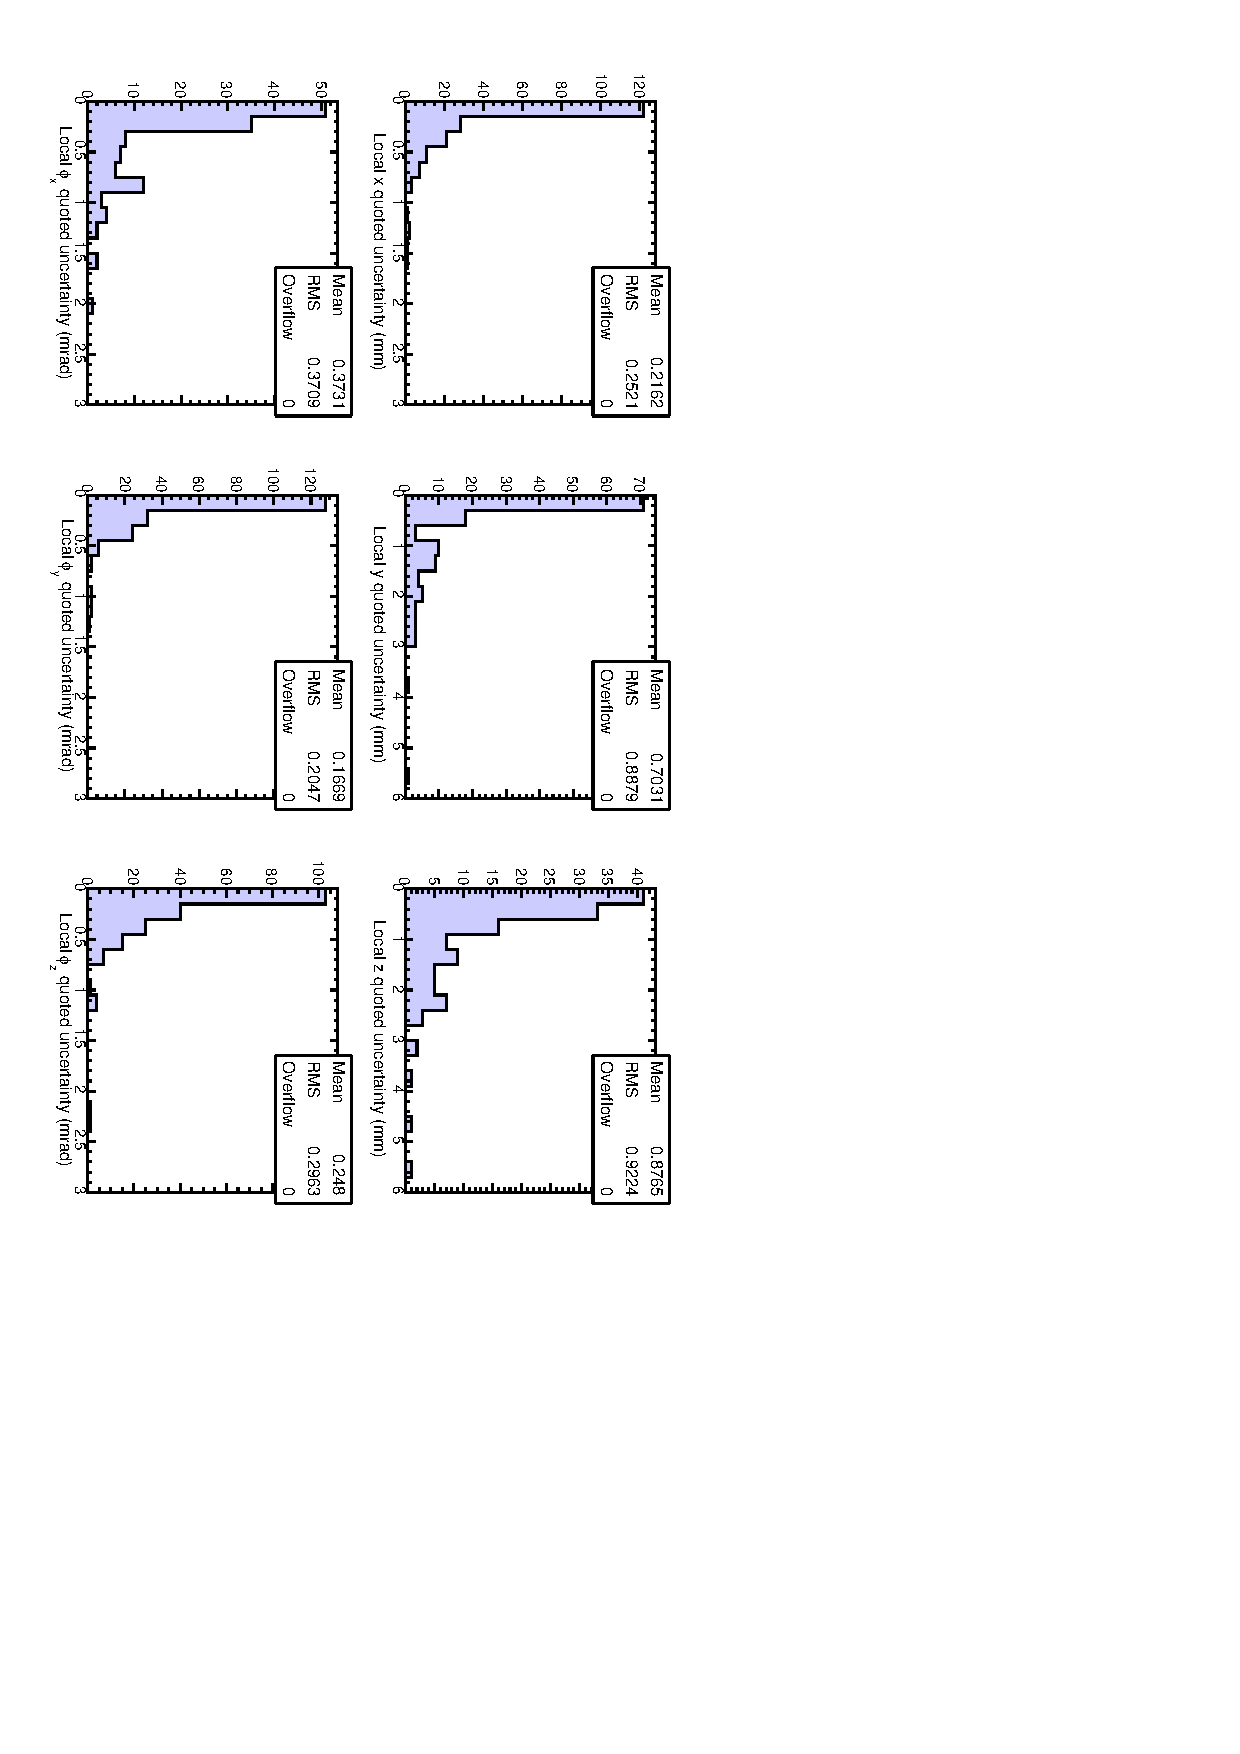
\includegraphics[height=\linewidth, angle=90]{data_quoted_uncertainty.pdf}
\end{frame}

\begin{frame}
\frametitle{Study: allow TID/TEC}

\begin{itemize}
\item Exclusion of TID/TEC tracker hits was based on a November study
\item What changes if we repeat the analysis without \mbox{excluding TID/TEC?\hspace{-1 cm}}
\item For one thing, we reach more chambers in wheels $\pm$2\ldots
\end{itemize}

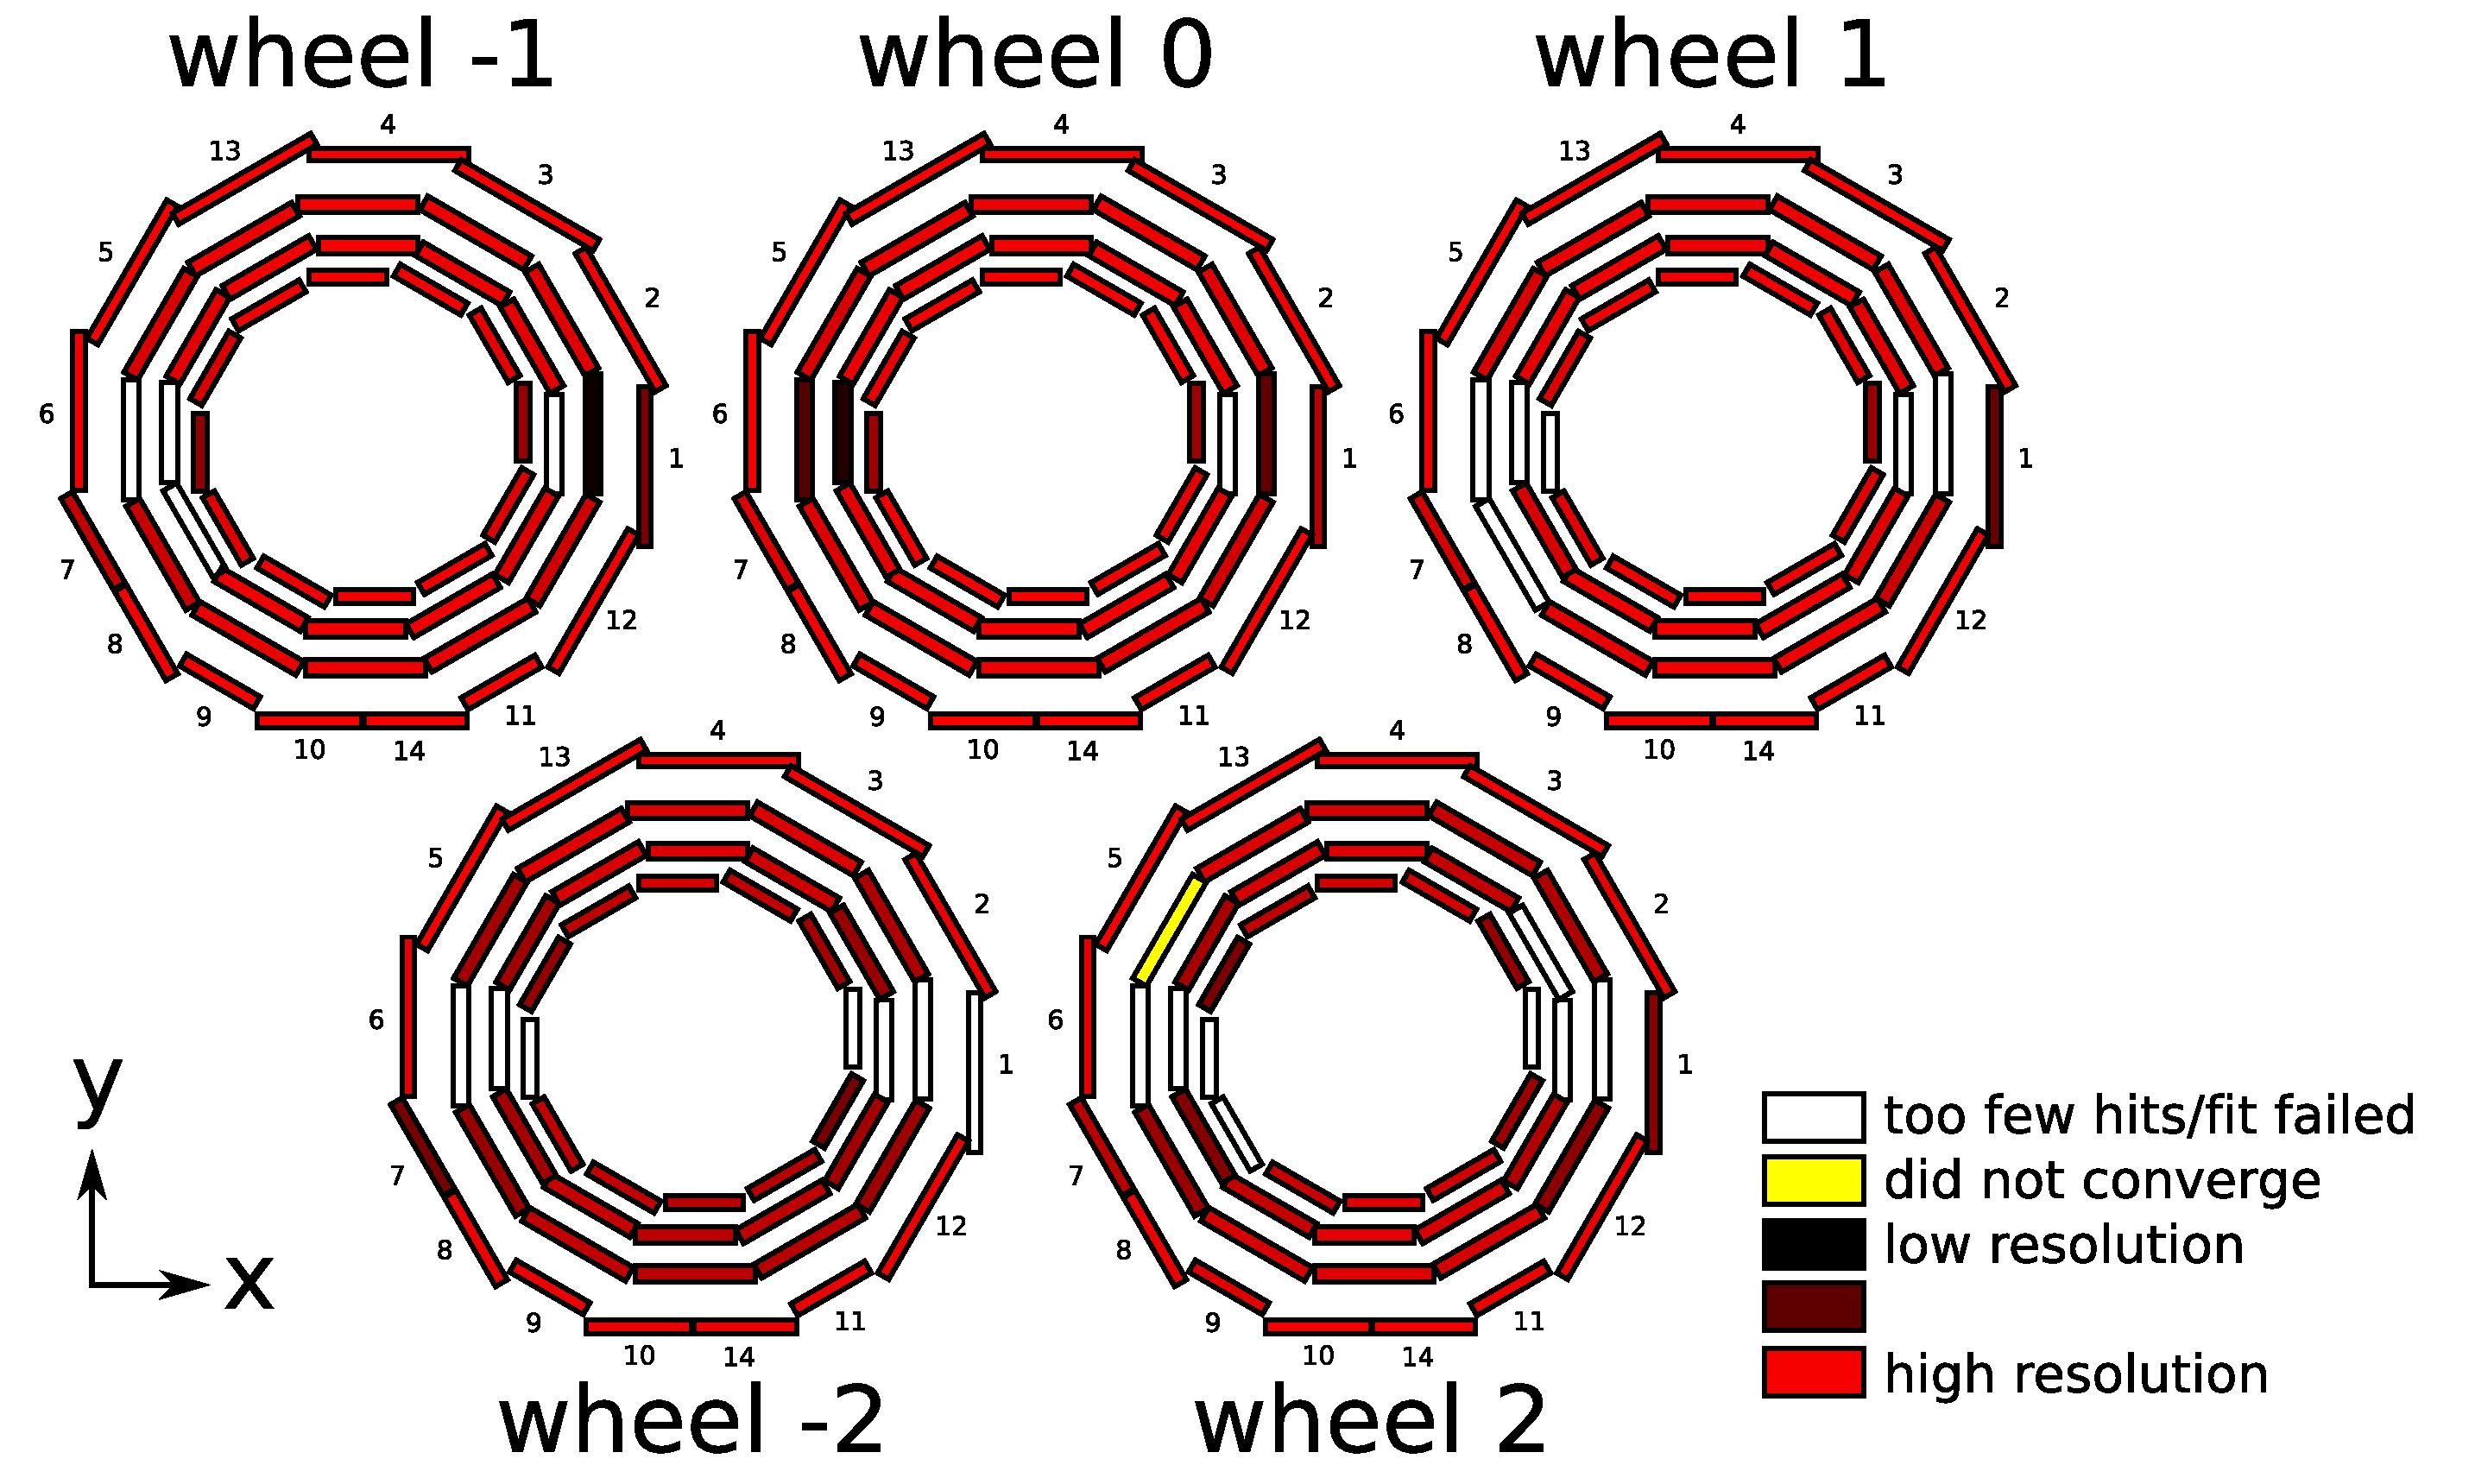
\includegraphics[width=\linewidth]{data_convergence_withTIDTEC.pdf}
\end{frame}

\begin{frame}
\frametitle{Study: allow TID/TEC}

\begin{itemize}
\item How do individual parameters change for individual chambers? (database comparison: TID/TEC excluded minus \mbox{TID/TEC allowed)\hspace{-1 cm}}
\item Biggest differences in wheels $\pm$2, mostly in local $\delta_y$/$\delta_z$\ldots
\end{itemize}

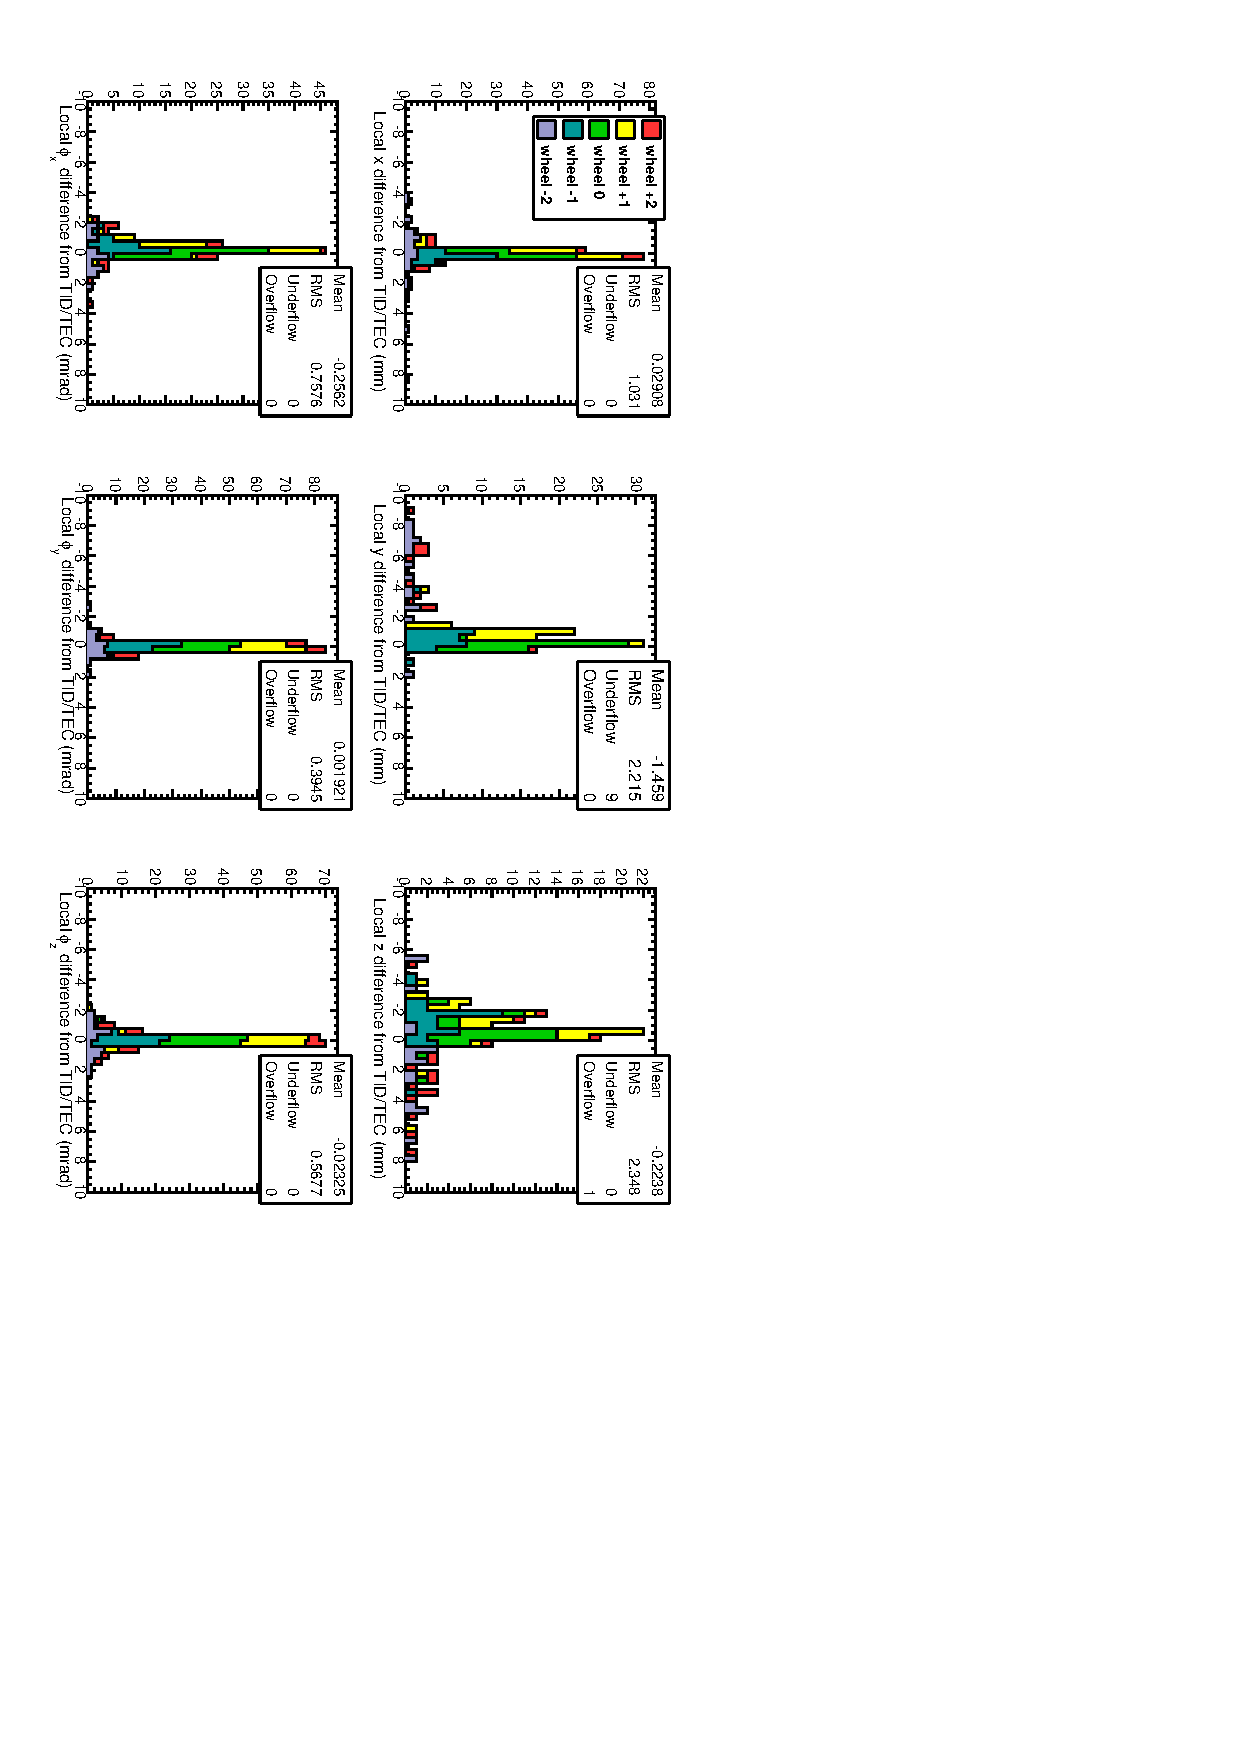
\includegraphics[height=\linewidth, angle=90]{data_effect_of_TIDTEC_all.pdf}
\end{frame}

\begin{frame}
\frametitle{Study: allow TID/TEC}

\begin{itemize}
\item What is the significance of those changes? \\ (difference over quoted uncertainty)
\item Large differences in wheel $\pm$2 local $\delta_y$/$\delta_z$ was due to low statistics
\item We will still exclude TID/TEC anyway \\ (better for future studies of TID/TEC from the muon system)
\end{itemize}

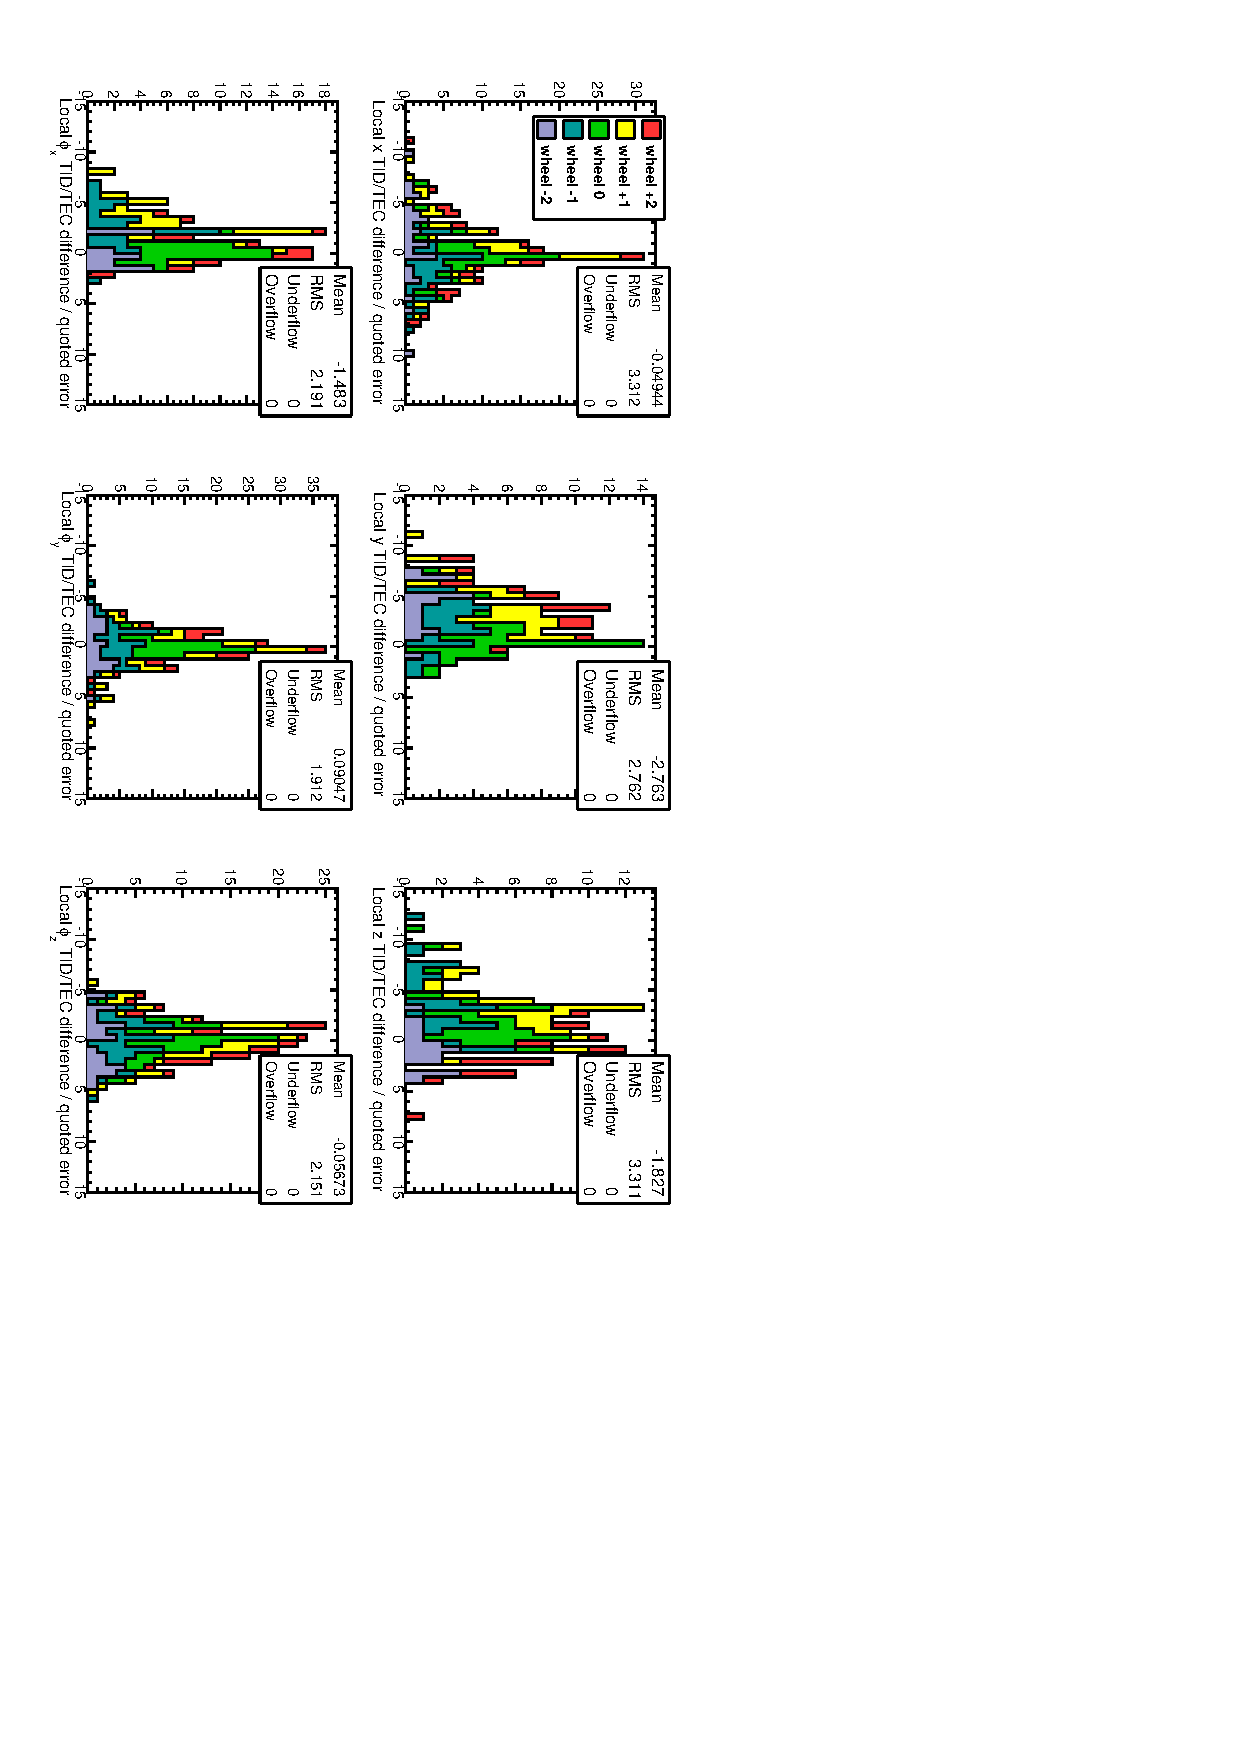
\includegraphics[height=\linewidth, angle=90]{data_effect_of_TIDTEC_norm.pdf}
\end{frame}

\begin{frame}
\frametitle{Production-quality alignment}

\begin{itemize}
\item Fix local $\delta_z = 0$ for all chambers
\item Fix local $\delta_y = 0$ for all chambers except wheel 0
\item Align only $\delta_x$, $\delta_{\phi_y}$, $\delta_{\phi_z}$ for station~4 because it's a 2-D device
\end{itemize}

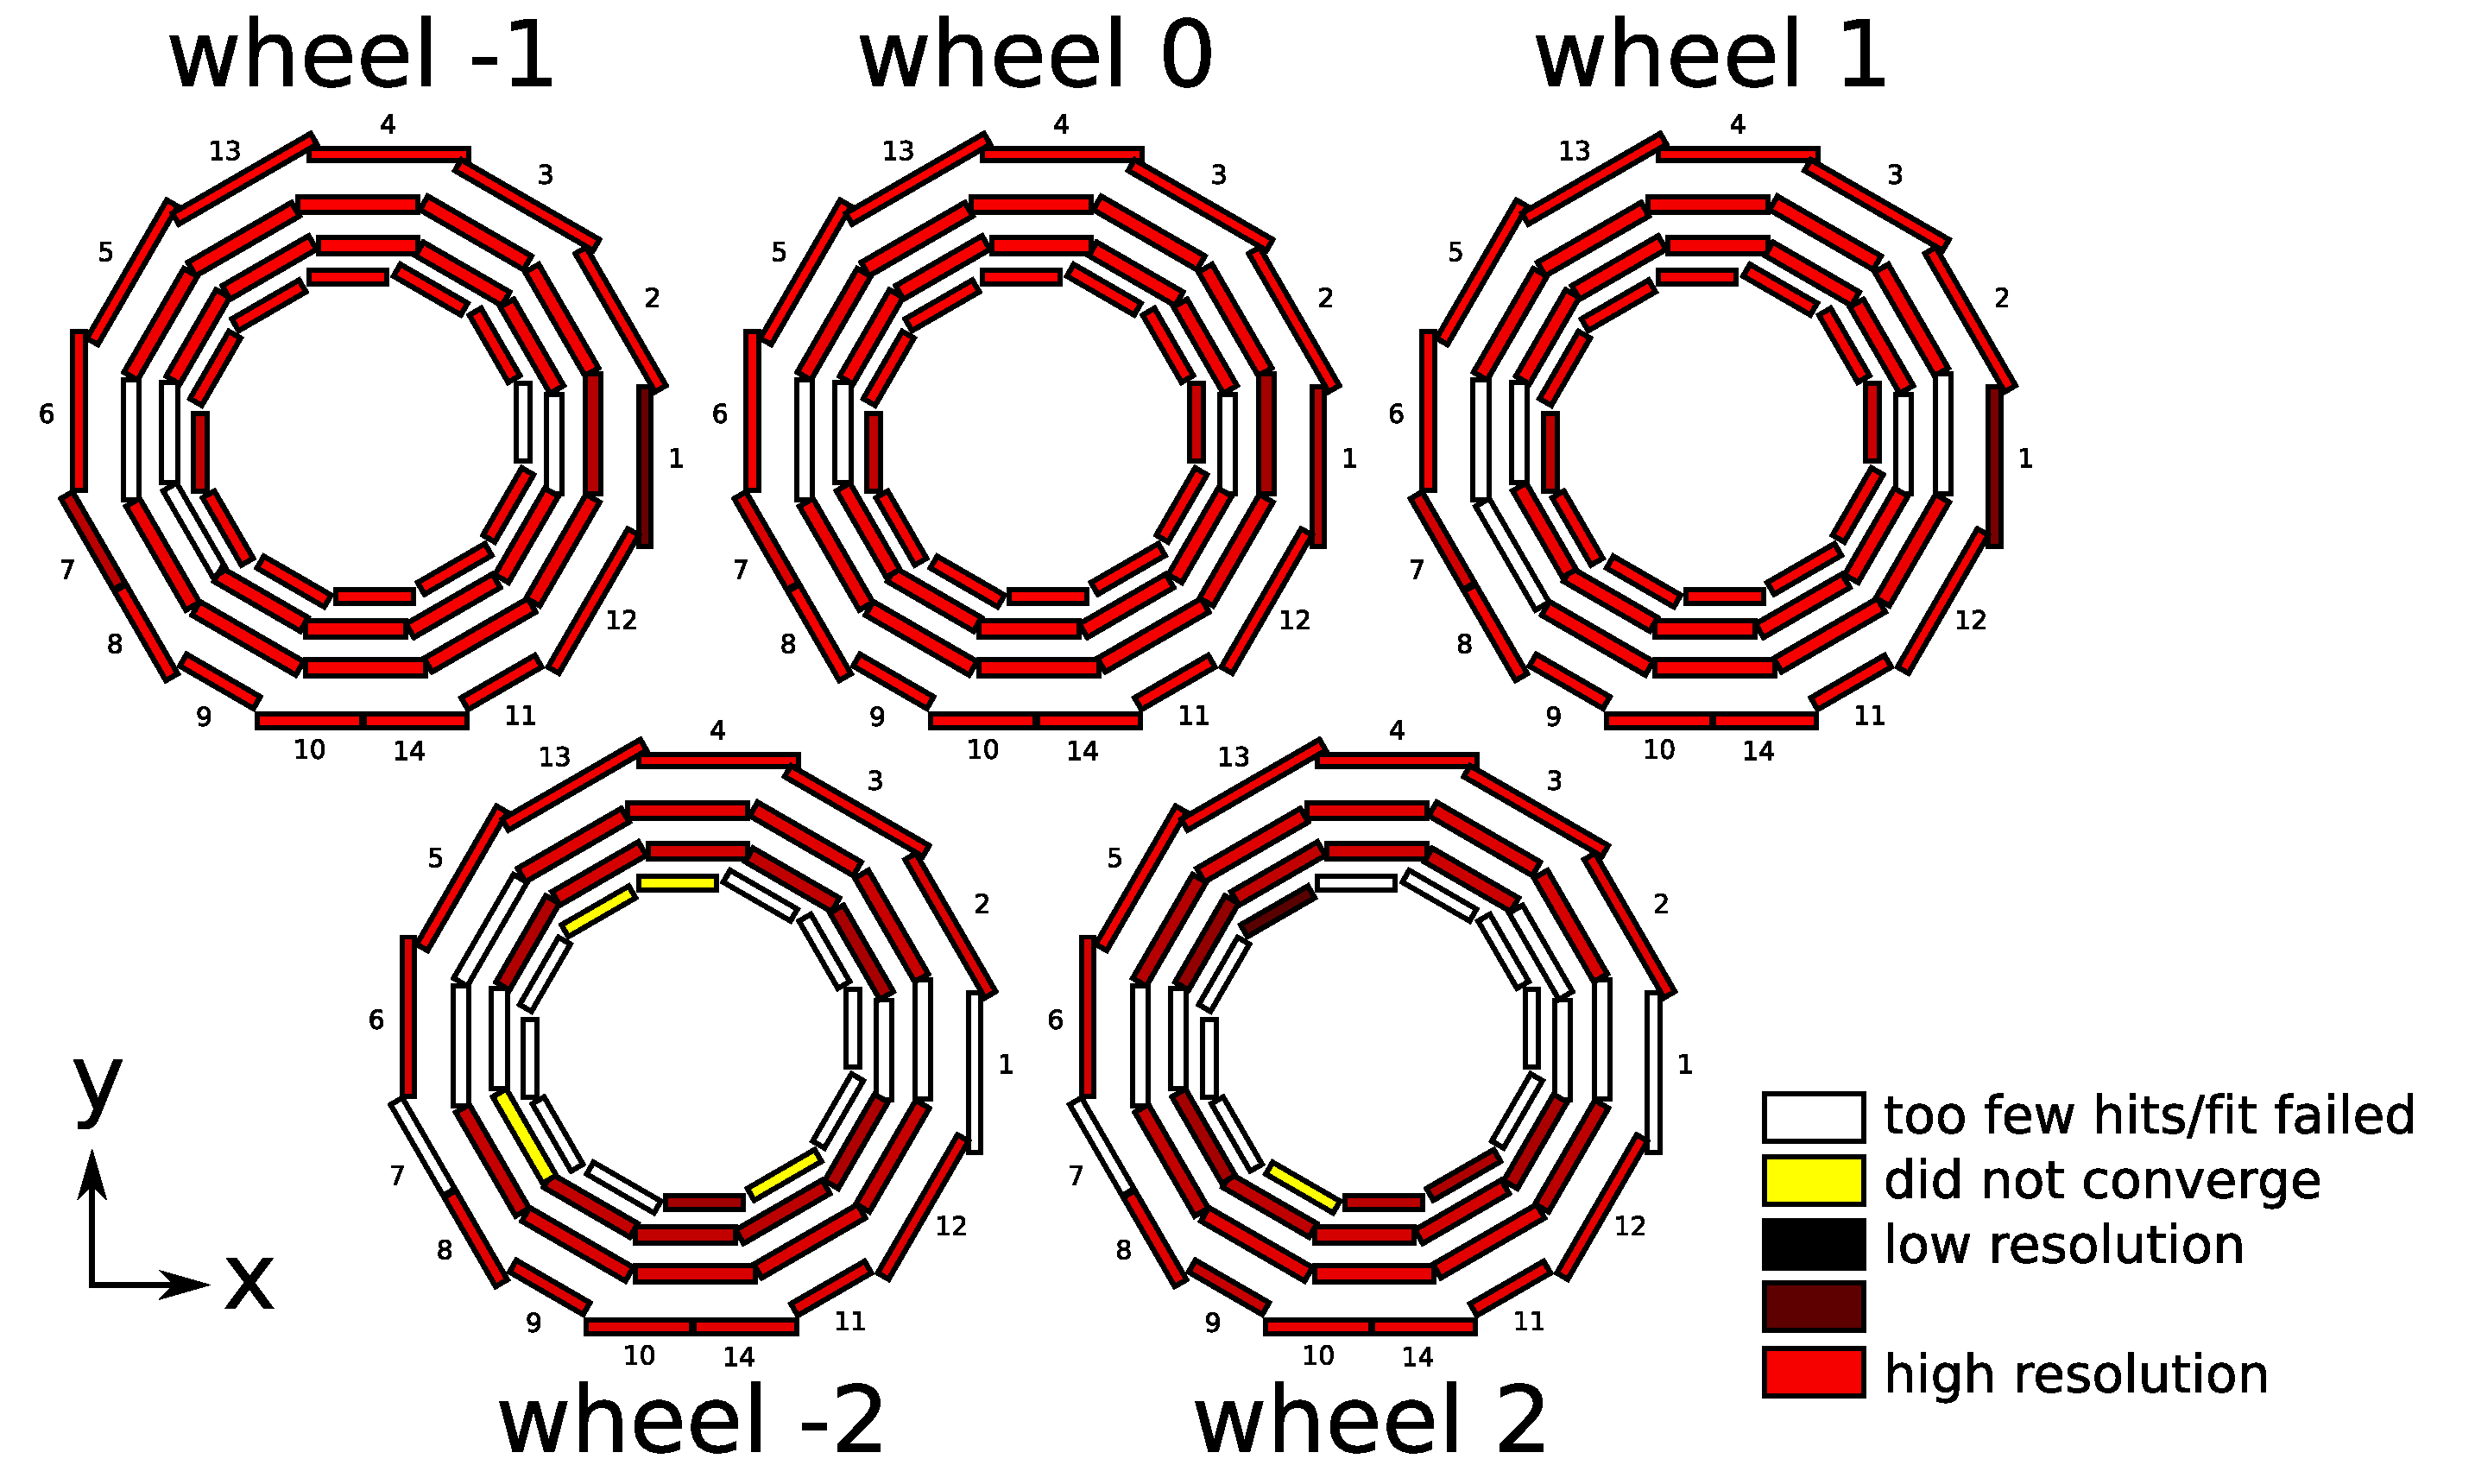
\includegraphics[width=\linewidth]{data_convergence_optimal.pdf}
\end{frame}

\begin{frame}
\frametitle{Effect of $\delta_y = \delta_z = 0$}

\begin{itemize}
\item Does that adversely affect other alignment paramters? \\ (database comparison: restricted DOF minus 6-DOF)
\item No, within 0.7~mm and 0.4~mrad
\end{itemize}

\vfill
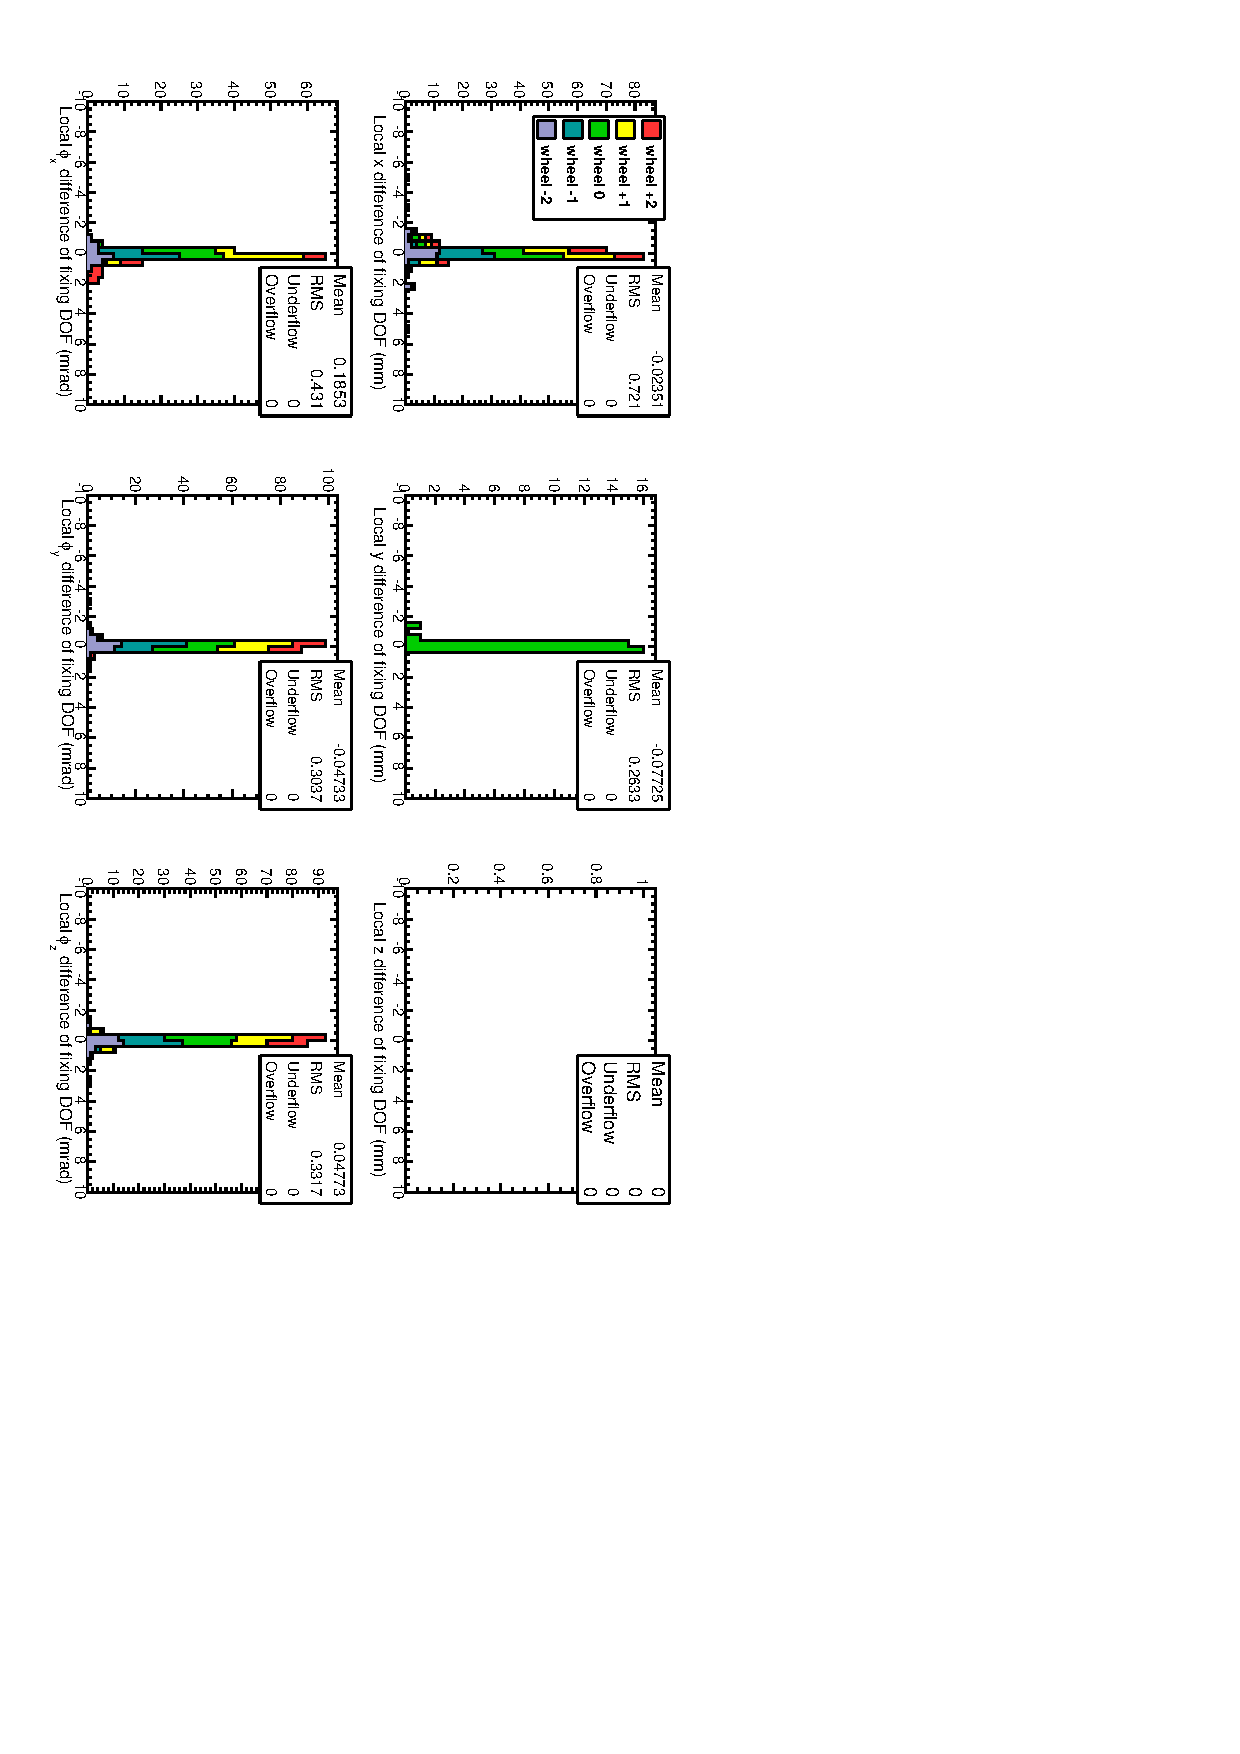
\includegraphics[height=\linewidth, angle=90]{data_effect_of_fixingdof.pdf}
\end{frame}

\begin{frame}
\frametitle{Significance of $\delta_y = \delta_z = 0$}

\begin{itemize}
\item Check the same difference divided by quoted uncertainties
\item Most $\delta_x$ within one sigma, some differ by as much as 10~sigma
\item By comparison with the previous page, those sigmas $\ll$ 1~mm
\end{itemize}

\vfill
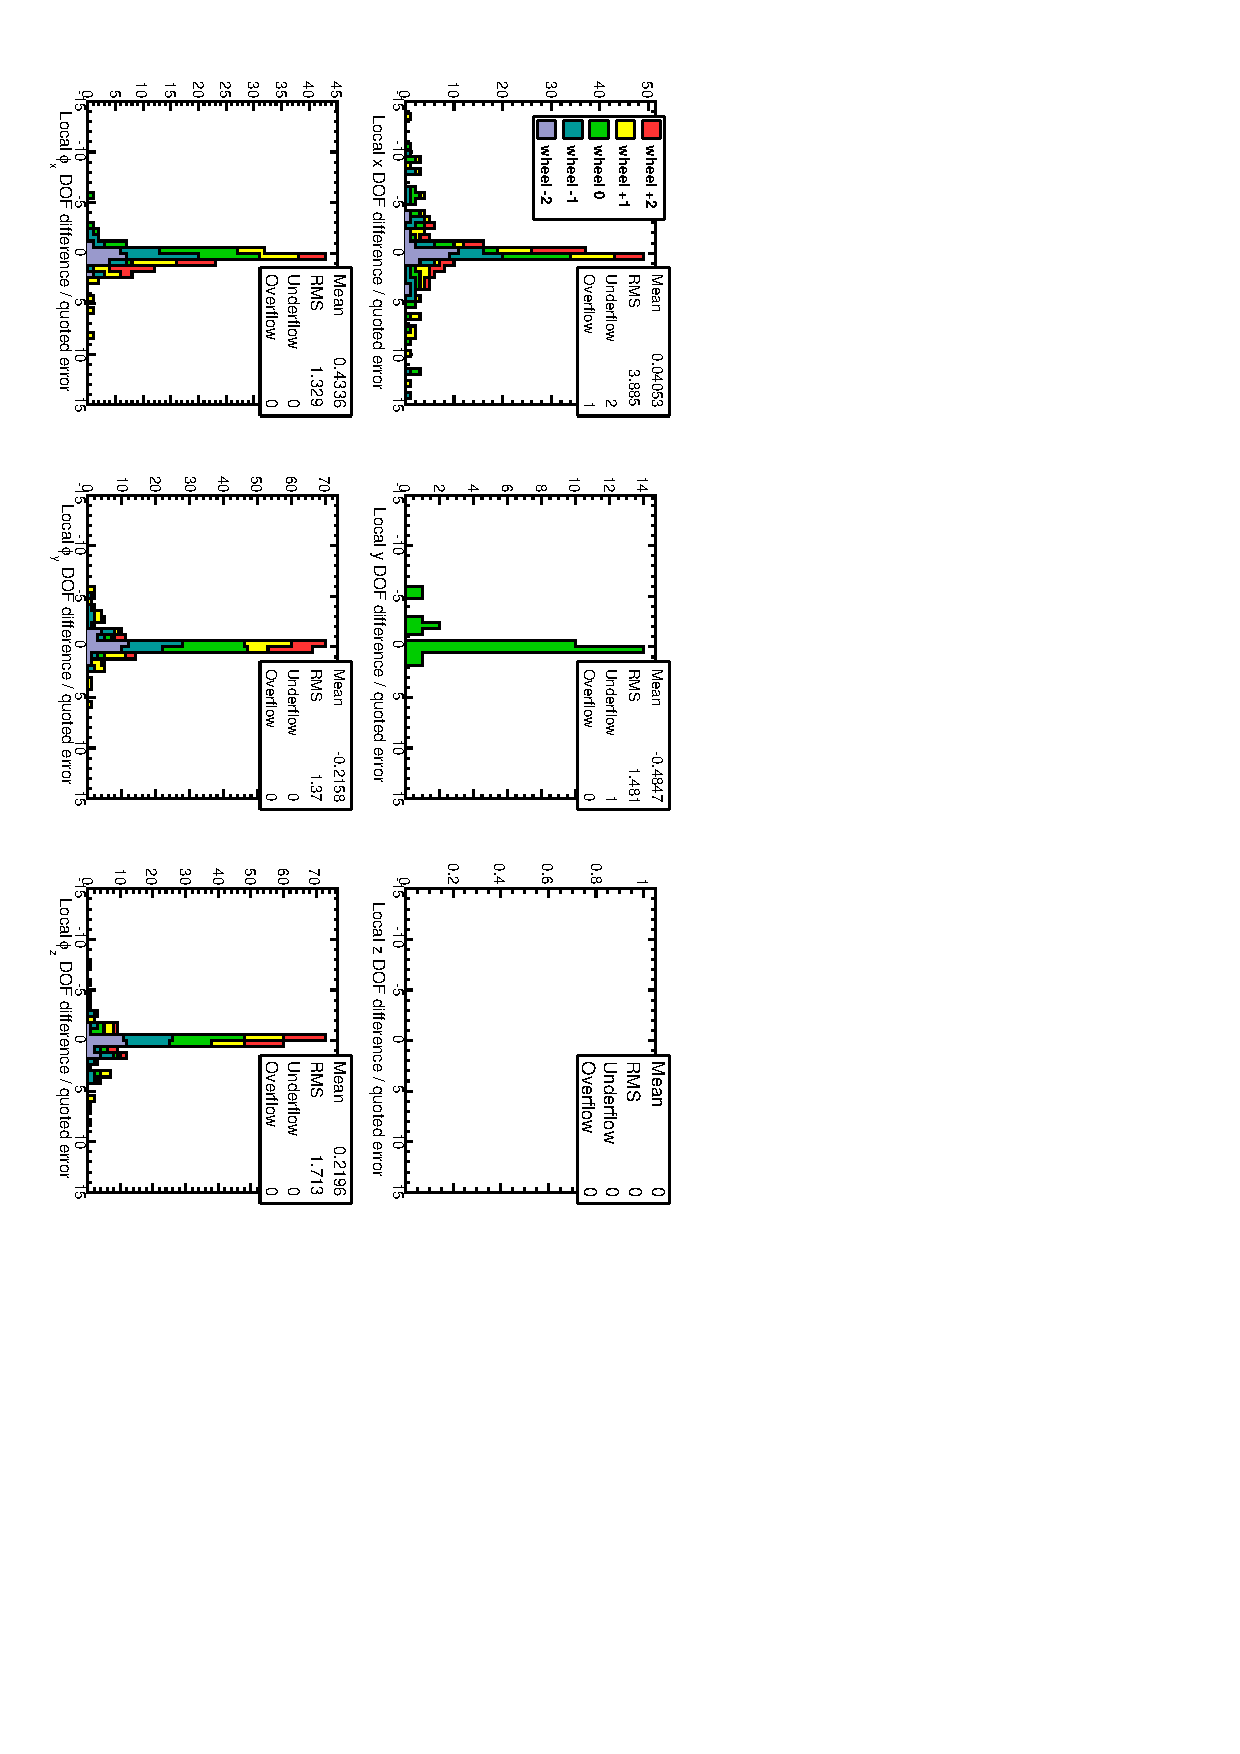
\includegraphics[height=\linewidth, angle=90]{data_effect_of_fixingdof_norm.pdf}
\end{frame}

\begin{frame}
\frametitle{Validation}
\framesubtitle{by which we mean checking that the procedure is valid: ``sanity checks''}

\begin{itemize}
\item Residuals distributions should get narrower, because we moved chambers to center their residuals distributions
\item A summary must fit on 1--2 slides (unlike 100's of ``map plots'')
\item But raw residuals are too wide to see the new corrections
\begin{itemize}\setlength{\itemsep}{0.1 cm}
\item e.g.\ $\delta_x$ corrections hidden under 7~mm $\Delta x$
\item exception: new $\delta_{\phi_y}$ corrections can be seen in 5~mrad $\Delta \frac{dx}{dz}$
\end{itemize}
\end{itemize}

\begin{center}
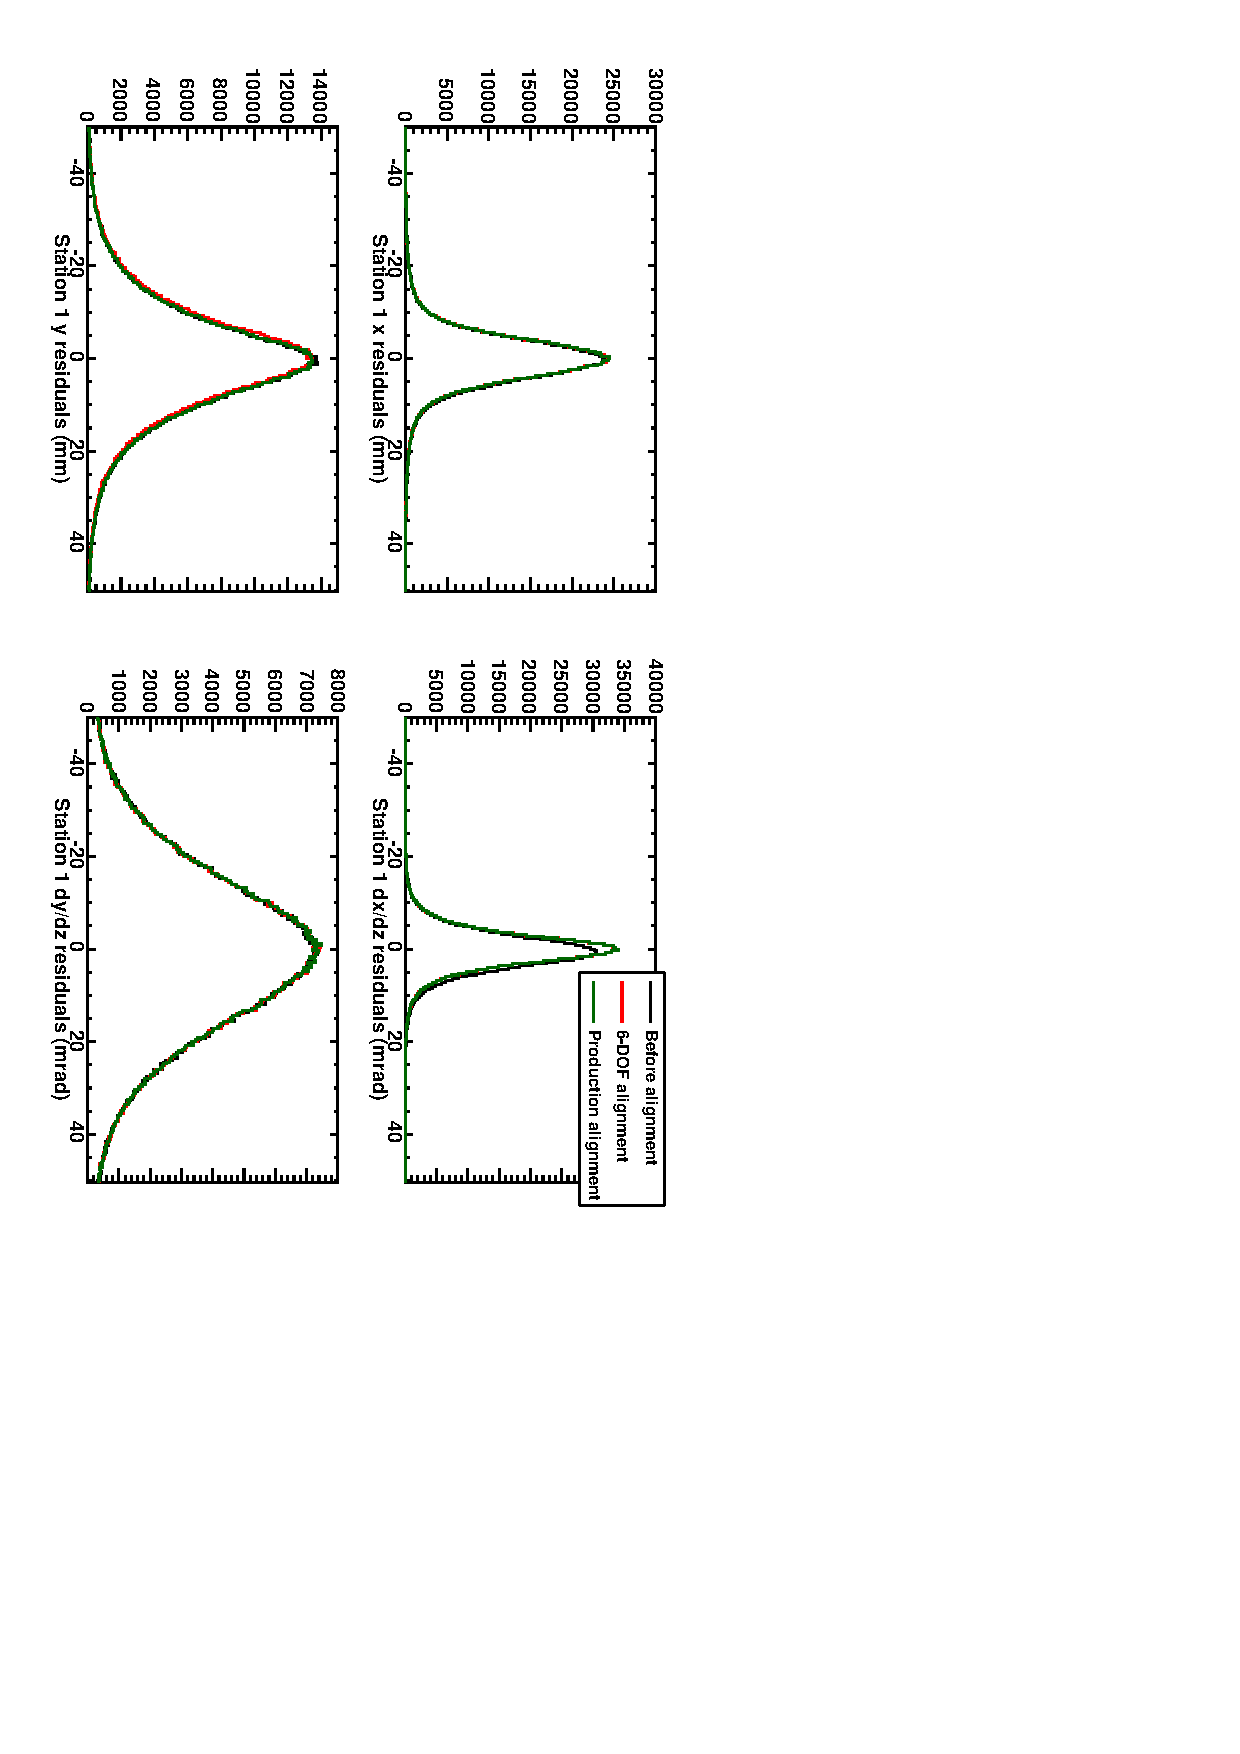
\includegraphics[height=0.8\linewidth, angle=90]{residuals_rawstation1.pdf}
\end{center}
\end{frame}

\begin{frame}
\frametitle{Refinement of validation}

\begin{itemize}
\item To see systematic alignment effects on residuals, we need to reduce the track-by-track variance
\item Cutting on $p_T$ reduces tails, but not the core width
\item Instead, note that $\Delta x$ and $\Delta \frac{dx}{dz}$ are correlated by physics:
\begin{itemize}\setlength{\itemsep}{0.1 cm}
\item small $|\Delta \frac{dx}{dz}|$ indicates that a track was measured well and did not scatter, and its {\it measurement} is independent of $\Delta x$
\item $\Delta x$ with $|\Delta \frac{dx}{dz}| < 1$~mrad is highly sensitive to \mbox{$\delta_x$ misalignments\hspace{-1 cm}}
\end{itemize}

\end{itemize}

\begin{columns}
\column{0.5\linewidth}

\vspace{-0.5 cm}
Using the familiar correlation between $\Delta x$ and $\Delta \frac{dx}{dz}$:

\vspace{0.25 cm}
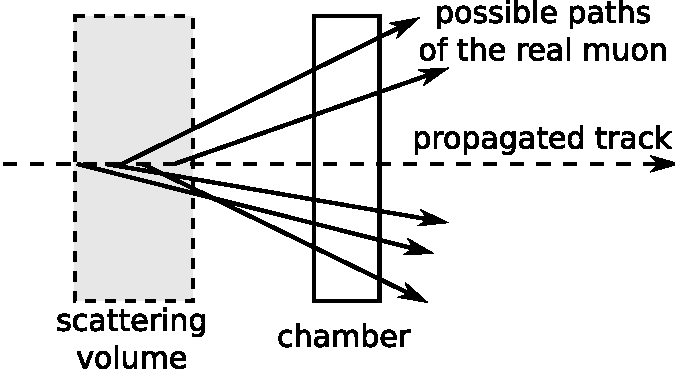
\includegraphics[width=\linewidth]{sawtooth_diagram.pdf}

\column{0.4\linewidth}

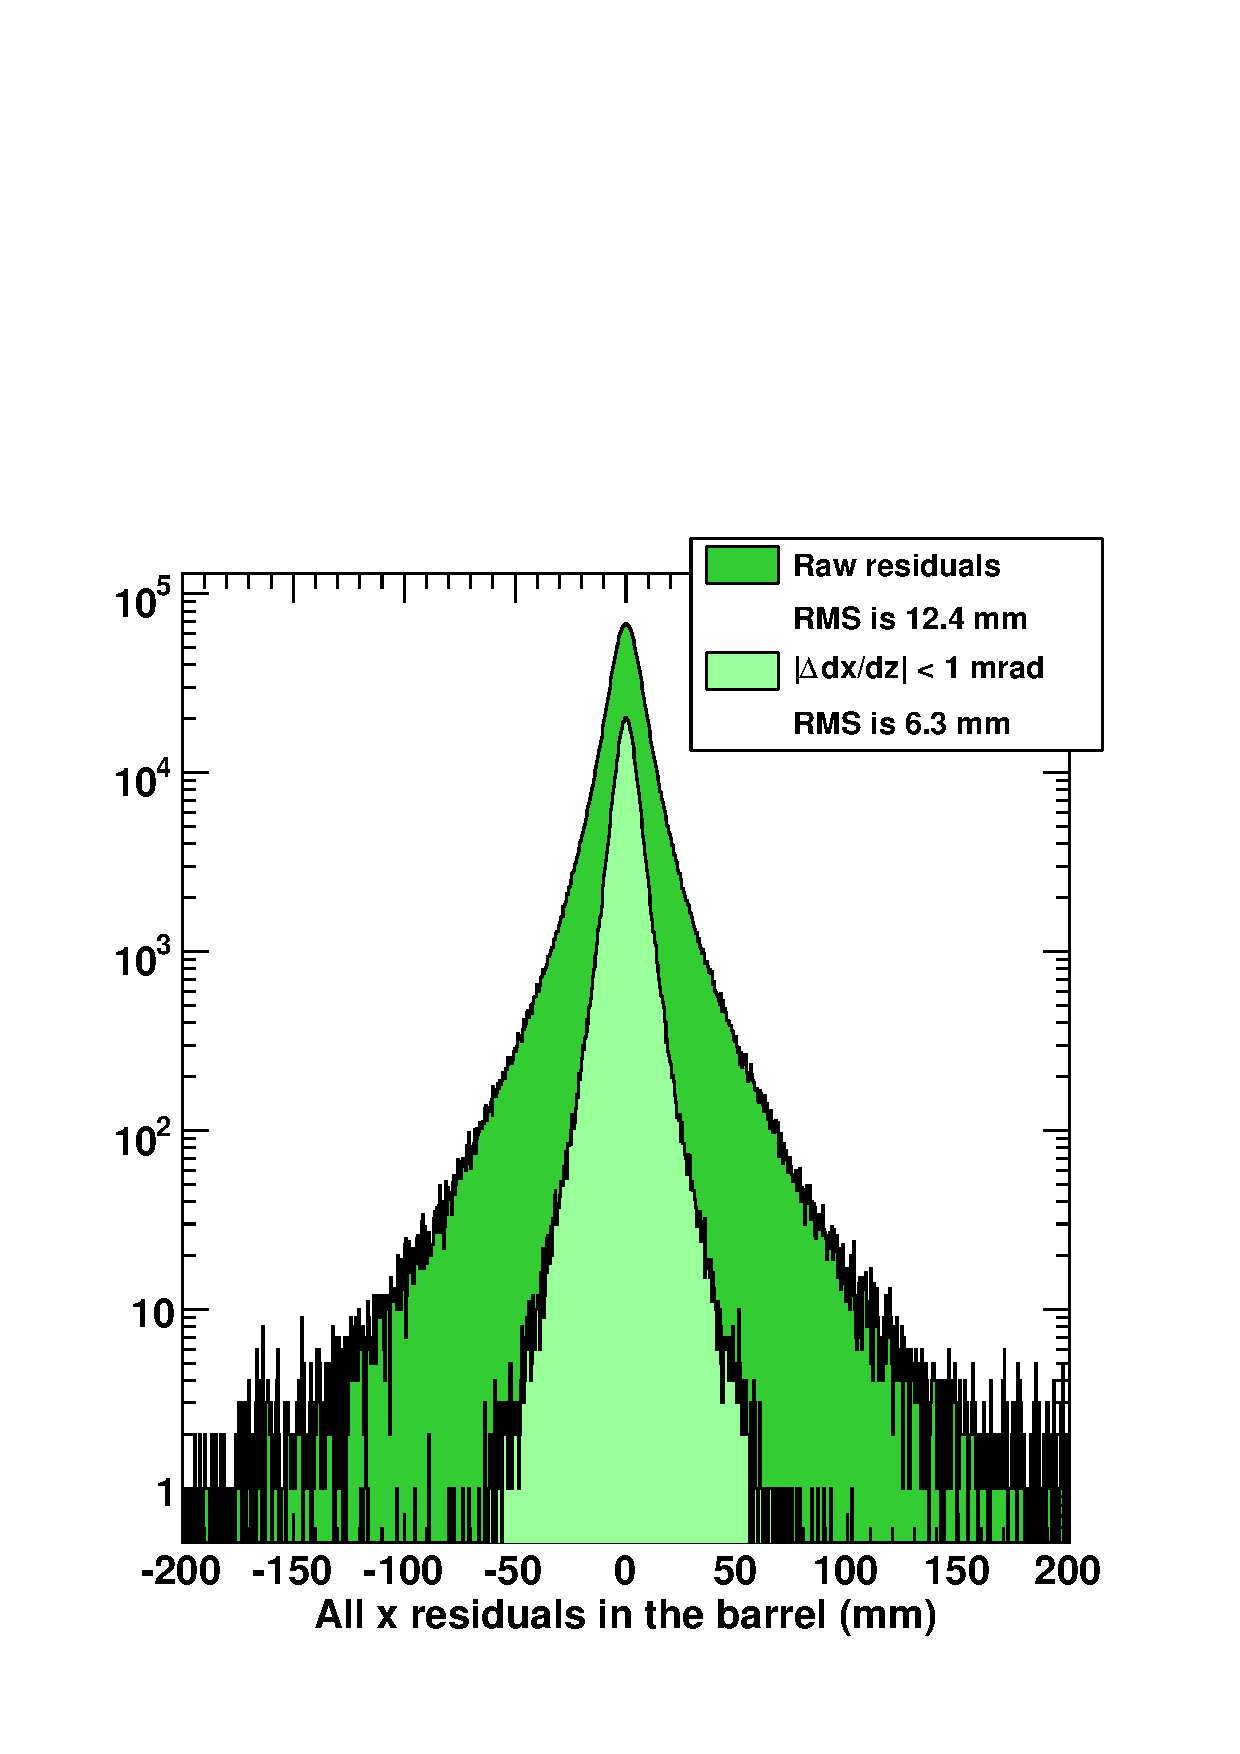
\includegraphics[width=\linewidth]{residuals_explanation.pdf}

\end{columns}
\end{frame}

\begin{frame}
\frametitle{Residuals with $|\Delta \frac{dx}{dz}| < 1$ mrad}

\begin{itemize}
\item With the track variance a factor of 2 narrower, we can now see the new $\delta_x$ corrections
\item But this validation only checks that we got what we asked for: global residuals closer to 0
\end{itemize}

\vfill
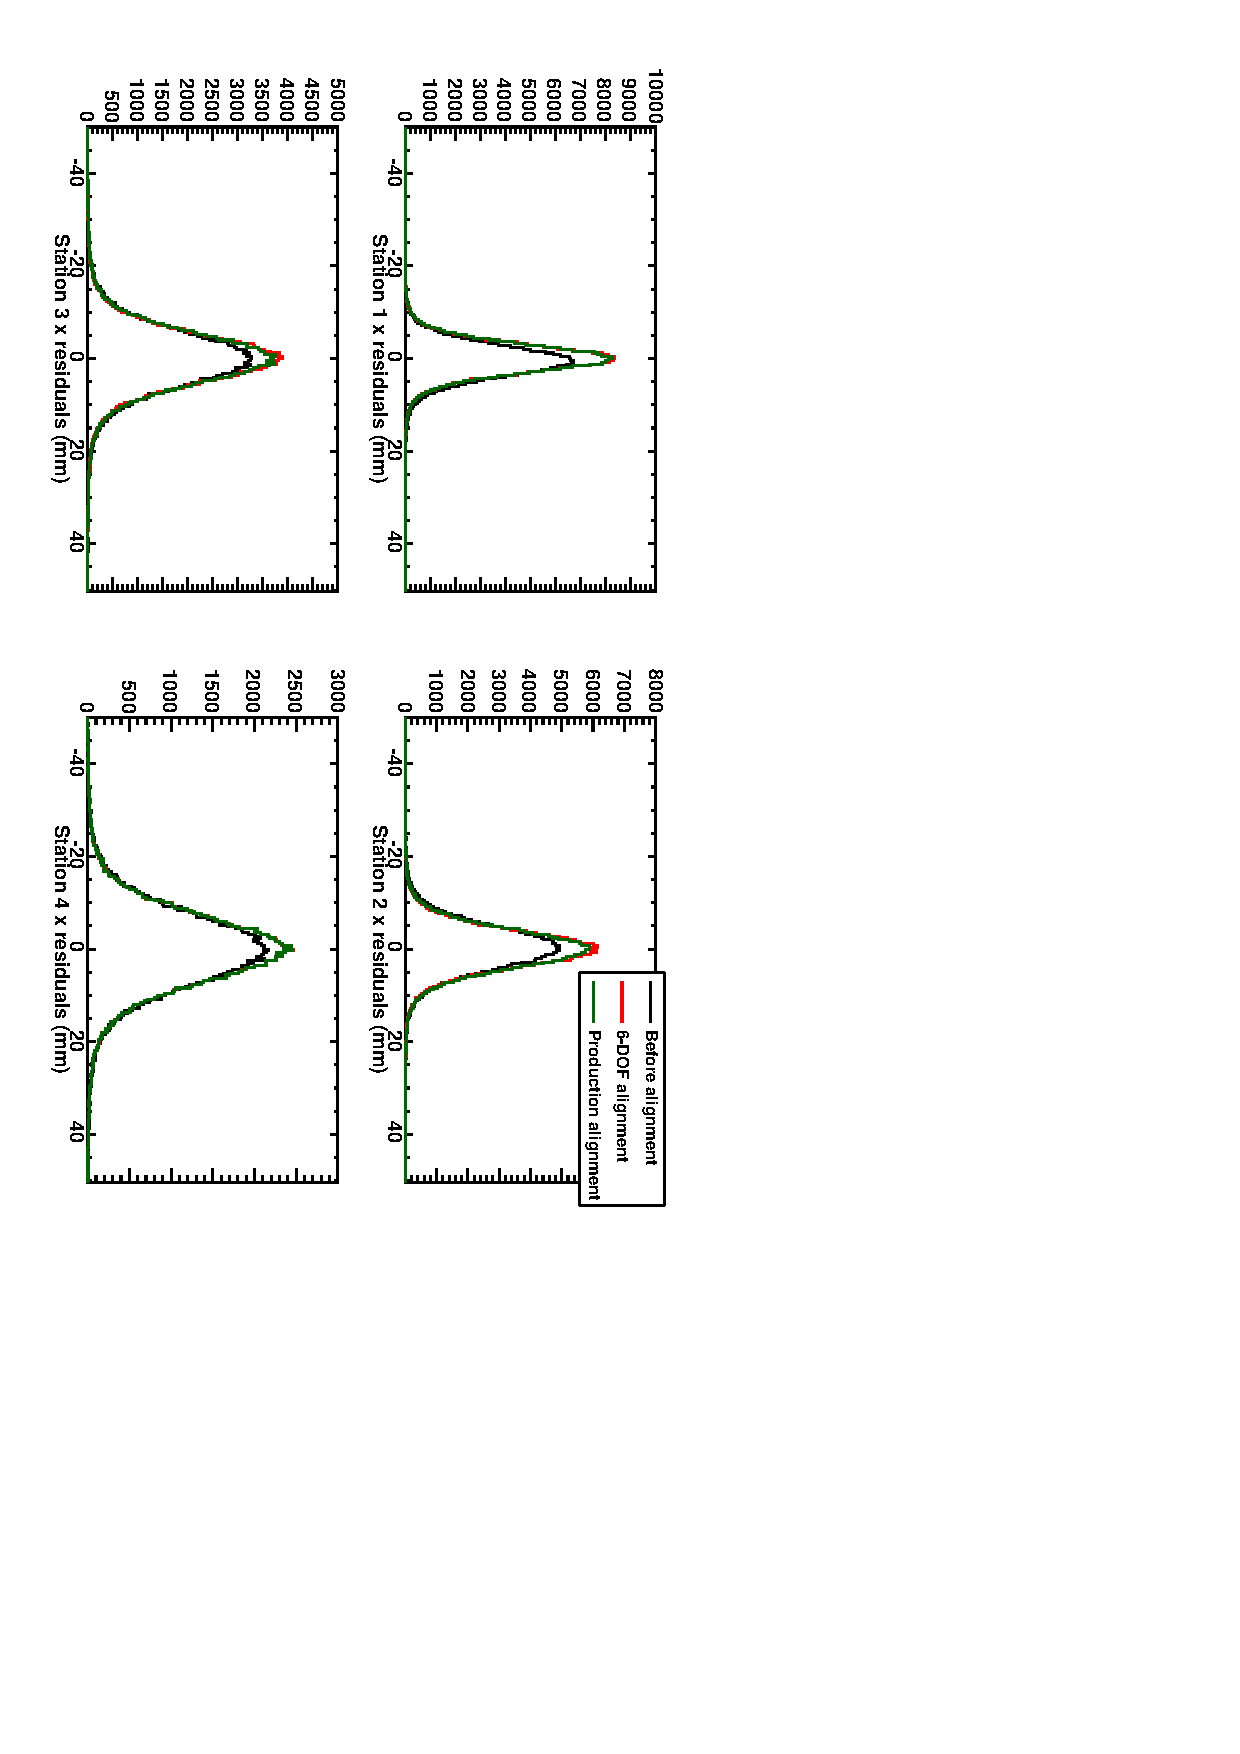
\includegraphics[height=\linewidth, angle=90]{residuals_cut1x.pdf}

\end{frame}

\begin{frame}
\frametitle{Verification}
\framesubtitle{by which we mean making sure that the aligned positions are {\it true}}

\begin{columns}
\column{0.3\linewidth}
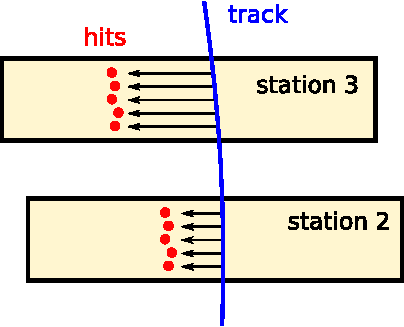
\includegraphics[width=\linewidth]{residuals_difference.pdf}

\column{0.7\linewidth}
\begin{itemize}
\item We aligned the global position of each chamber individually
\item If we look at differences in residuals, we will see relative
  alignment within sectors: new information that we did not use as a
  constraint (also higher precision)
\end{itemize}
\end{columns}

\begin{itemize}
\item With $|\Delta \frac{dx}{dz}| < 1$~mrad cut, dramatic improvement \mbox{in ${\Delta x}_{i+1} - {\Delta x}_i$\hspace{-1 cm}}
\item Best results with Production, even though 6-DOF \mbox{optimizes residuals!\hspace{-1 cm}}
\end{itemize}

\begin{columns}
\column{0.33\linewidth}
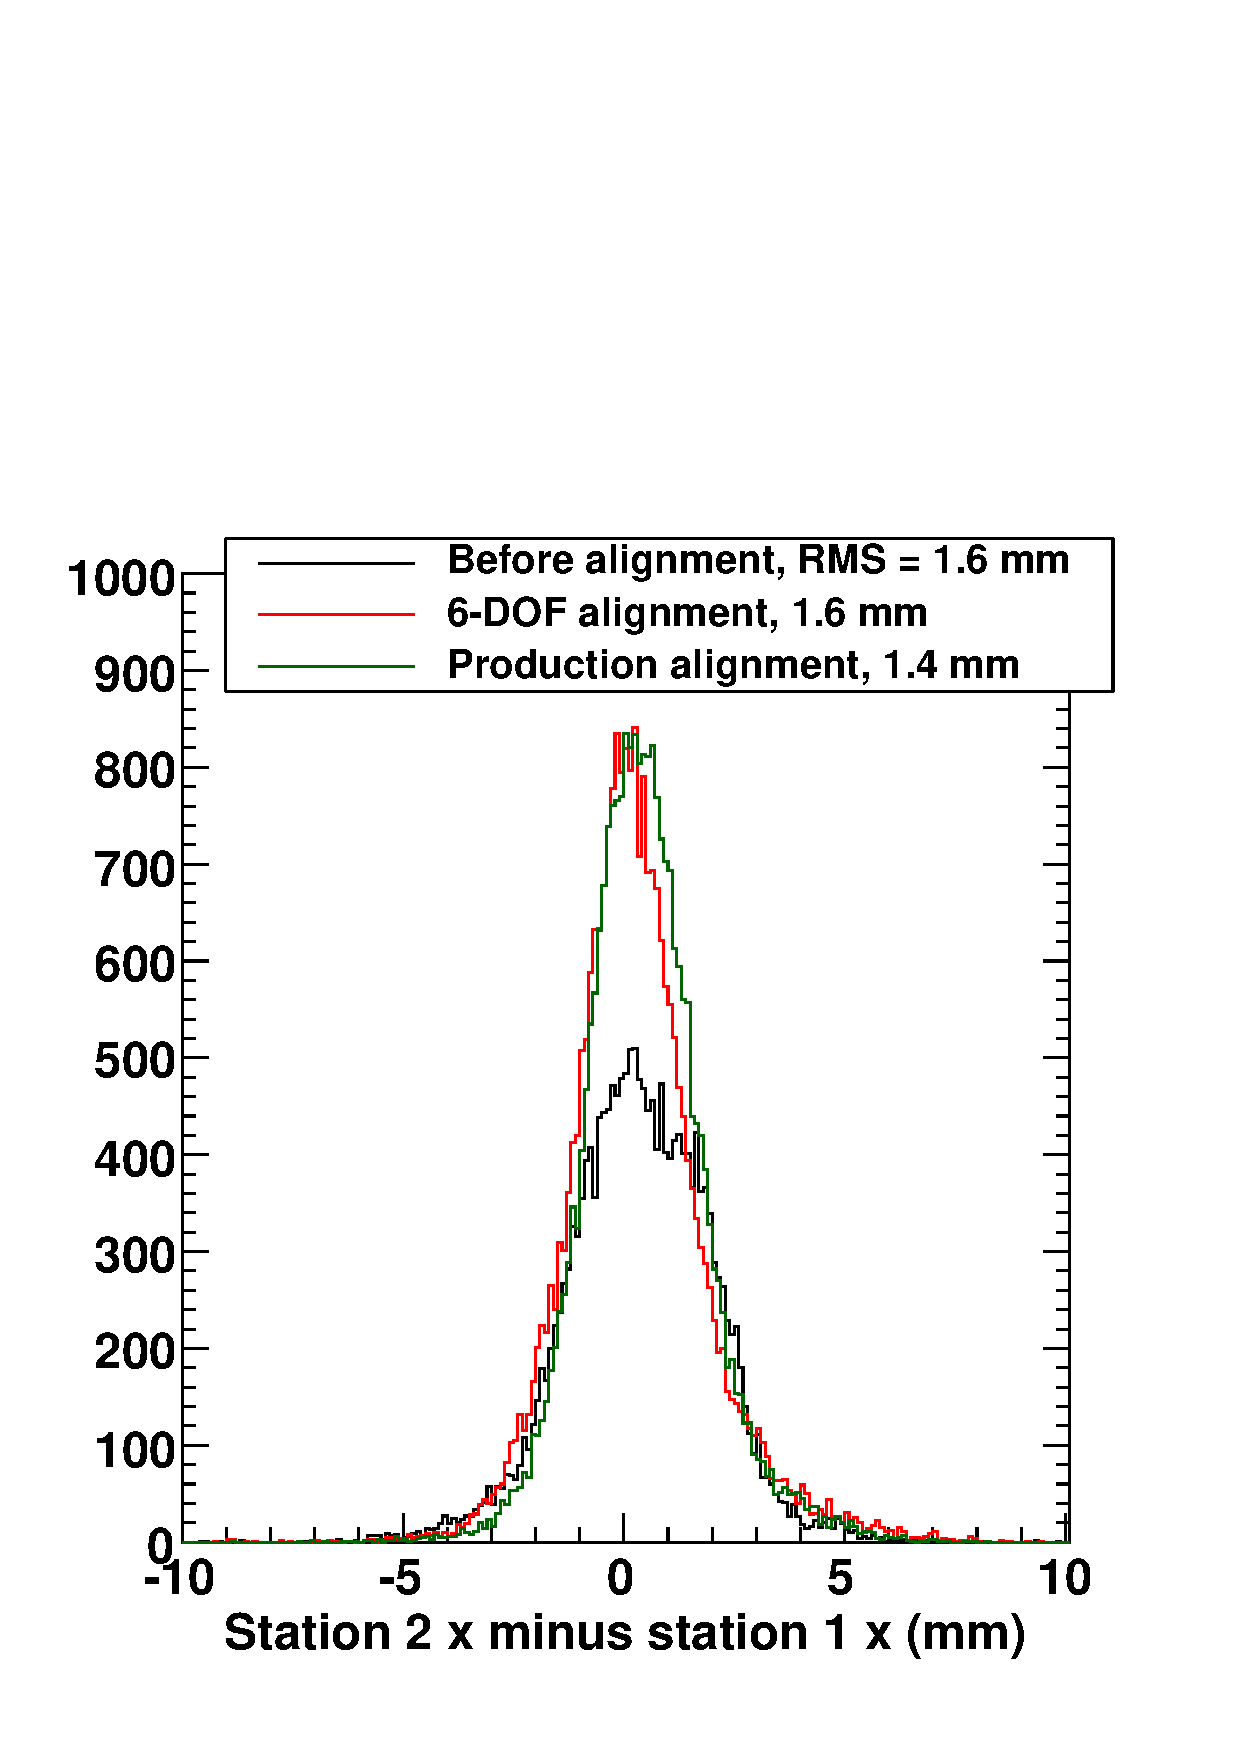
\includegraphics[width=\linewidth]{residuals_xdifffid1cut_12.pdf}
\column{0.33\linewidth}
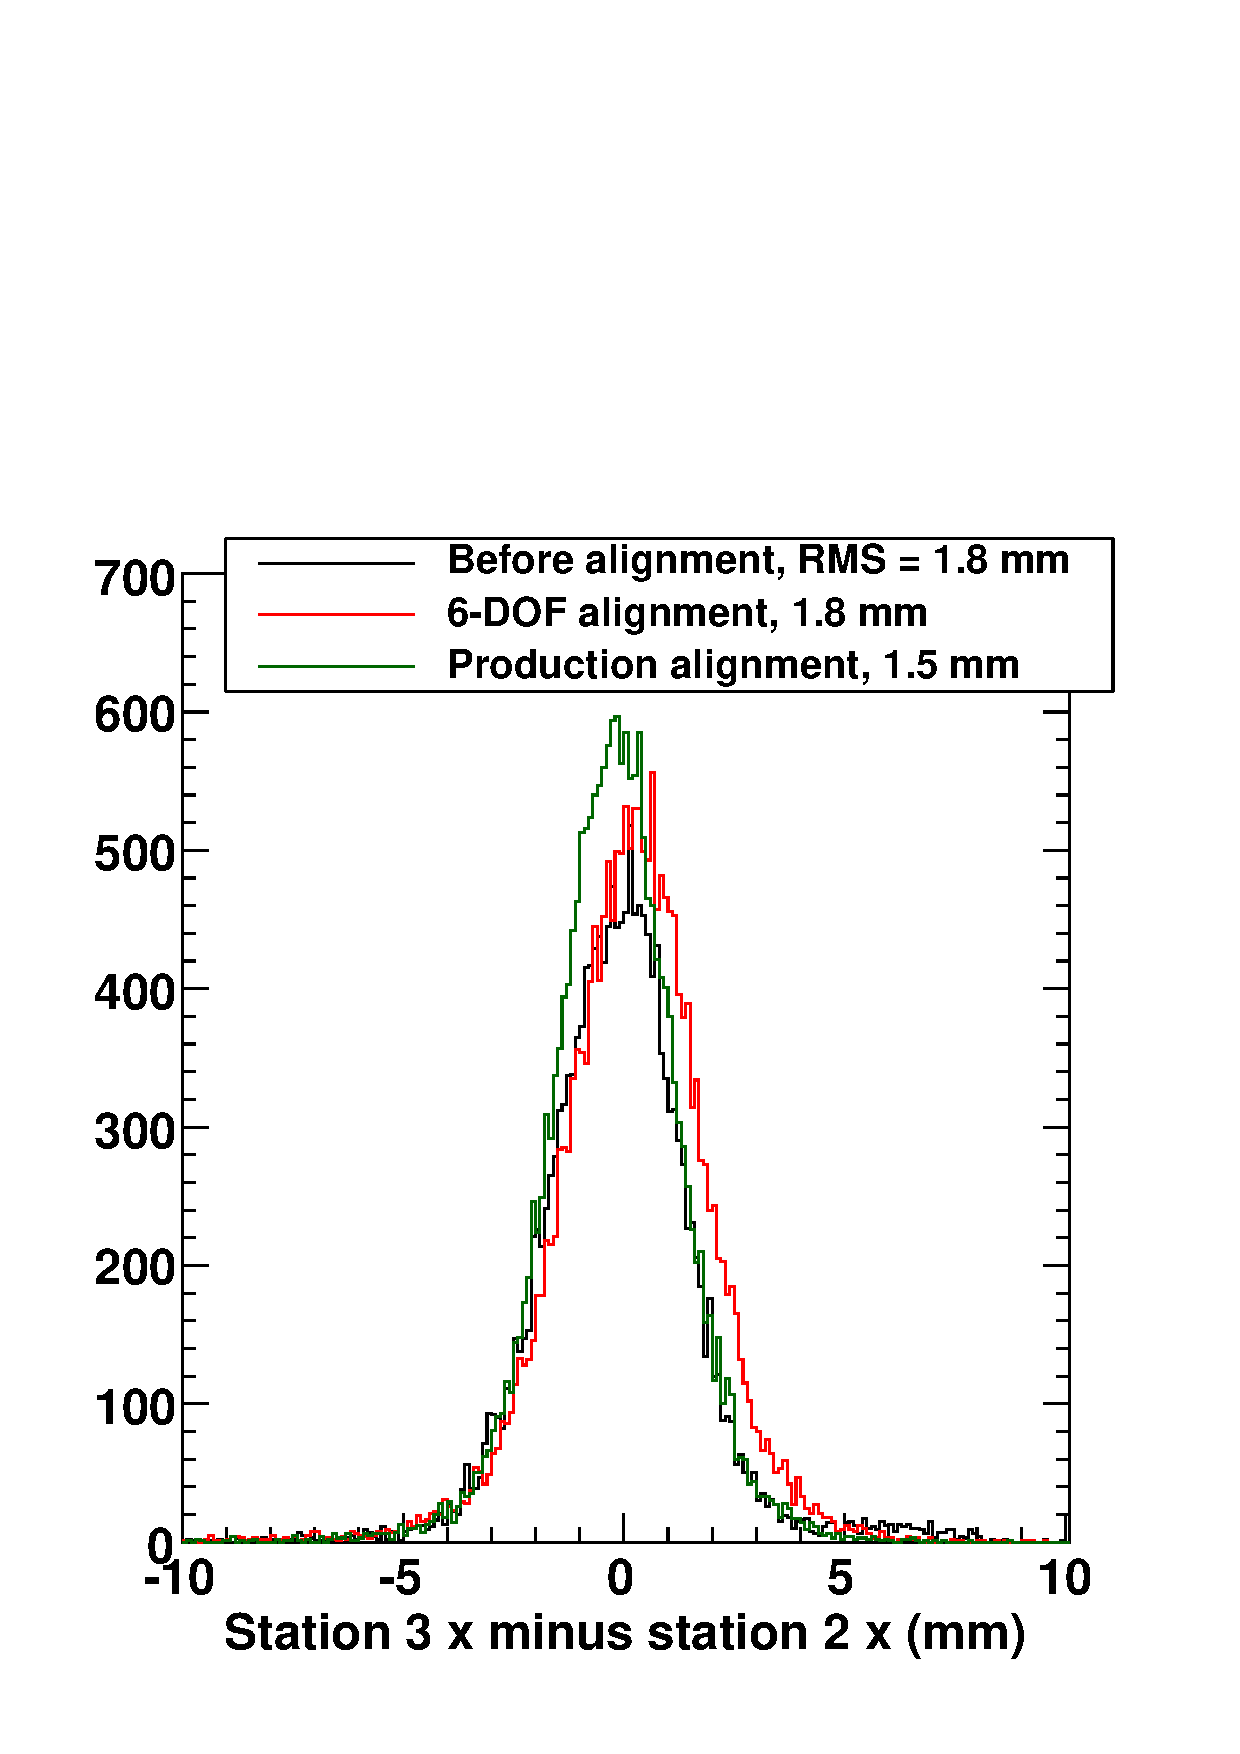
\includegraphics[width=\linewidth]{residuals_xdifffid1cut_23.pdf}
\column{0.33\linewidth}
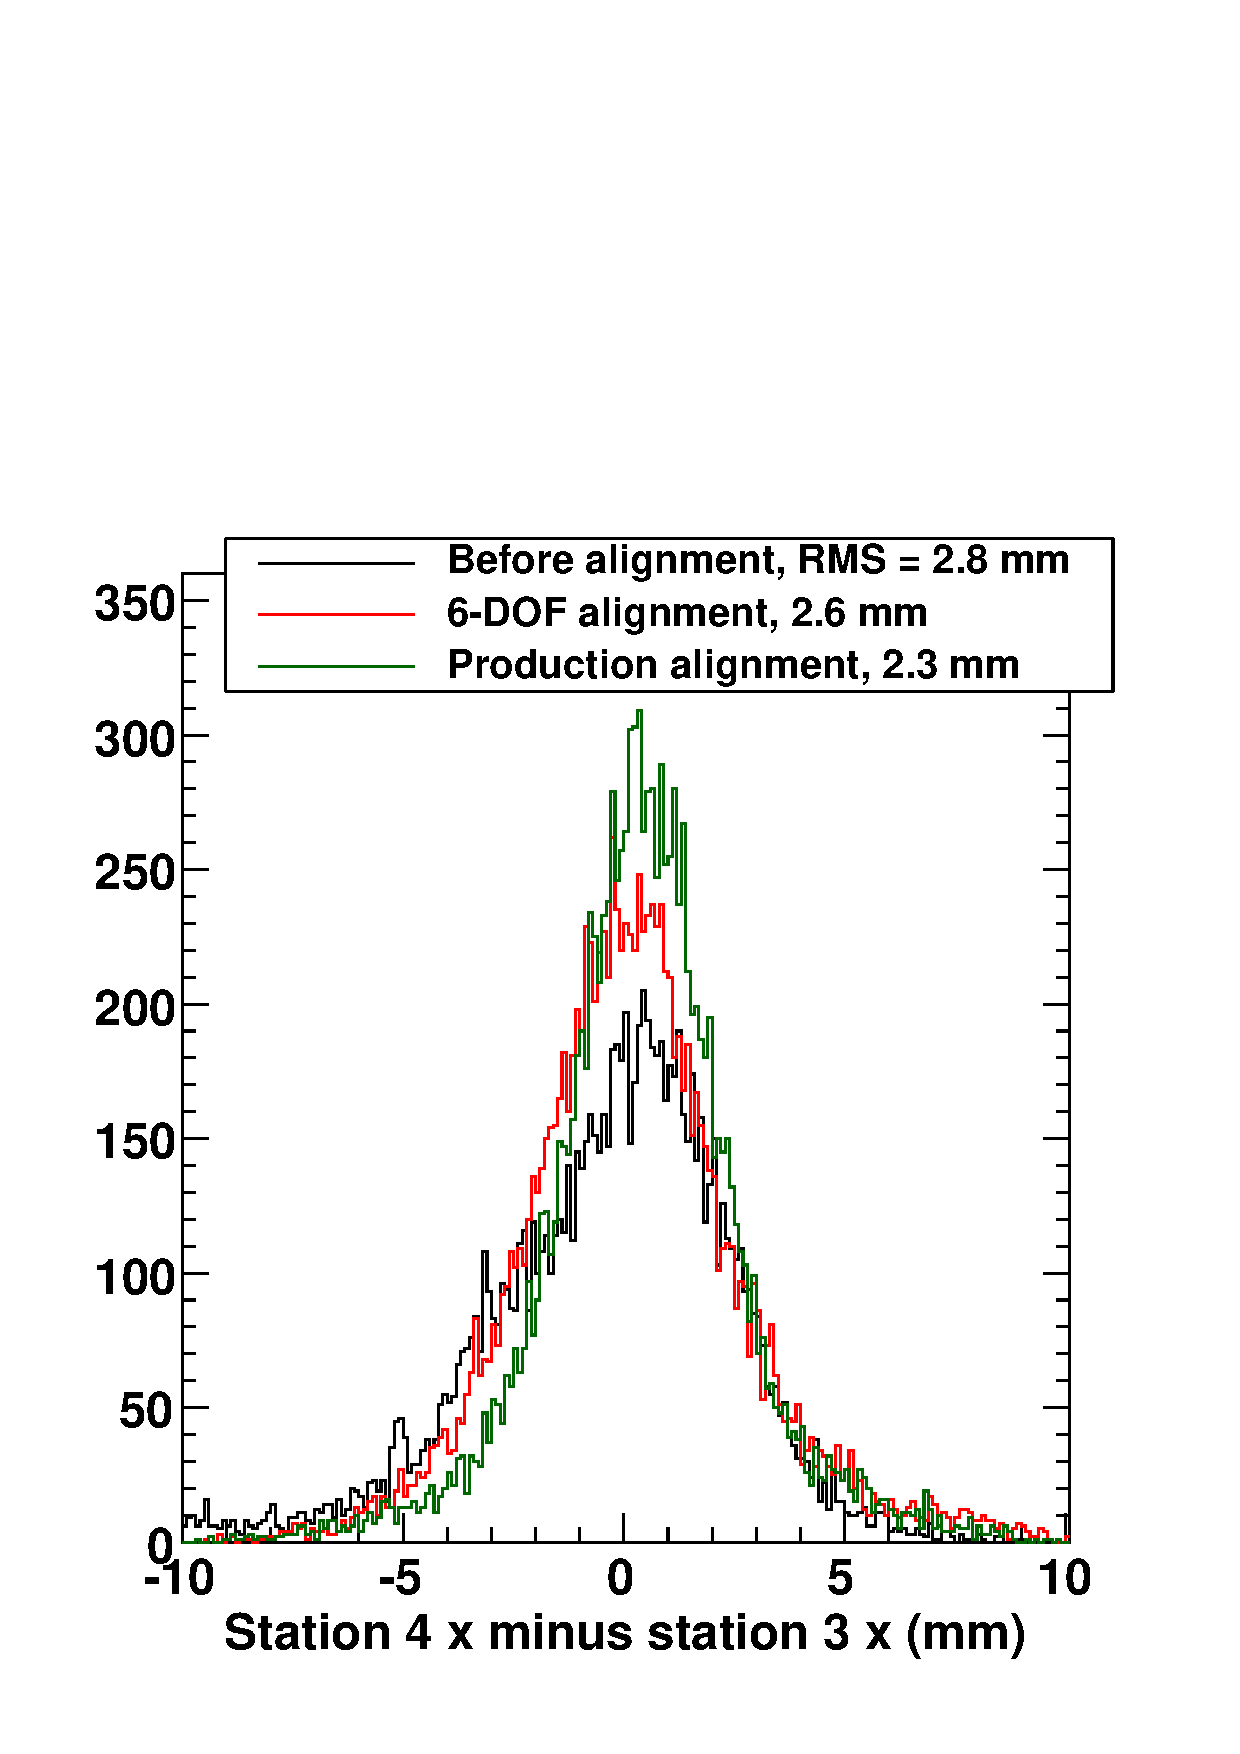
\includegraphics[width=\linewidth]{residuals_xdifffid1cut_34.pdf}
\end{columns}
\end{frame}

\begin{frame}
\frametitle{Proposal for TrackerPointing}

\begin{itemize}
\item From the Production alignment ($\delta_z = 0$ for all chambers, $\delta_y = 0$ in all wheels except~0, $\delta_y = \delta_{\phi_x} = 0$ for station~4),
\item Align only converged chambers with quoted uncertainties \\ $\sigma_x$ and $\sigma_y < 1$~mm, $\sigma_{\phi_x}$, $\sigma_{\phi_y}$, and $\sigma_{\phi_z} < 1$~mrad
\item Uses latest tracker alignment, APEs; independent \mbox{of TID/TEC\hspace{-1 cm}}
\item Contains track-based internal DT alignment (negotiable)
\end{itemize}

\begin{columns}
\column{0.5\linewidth}
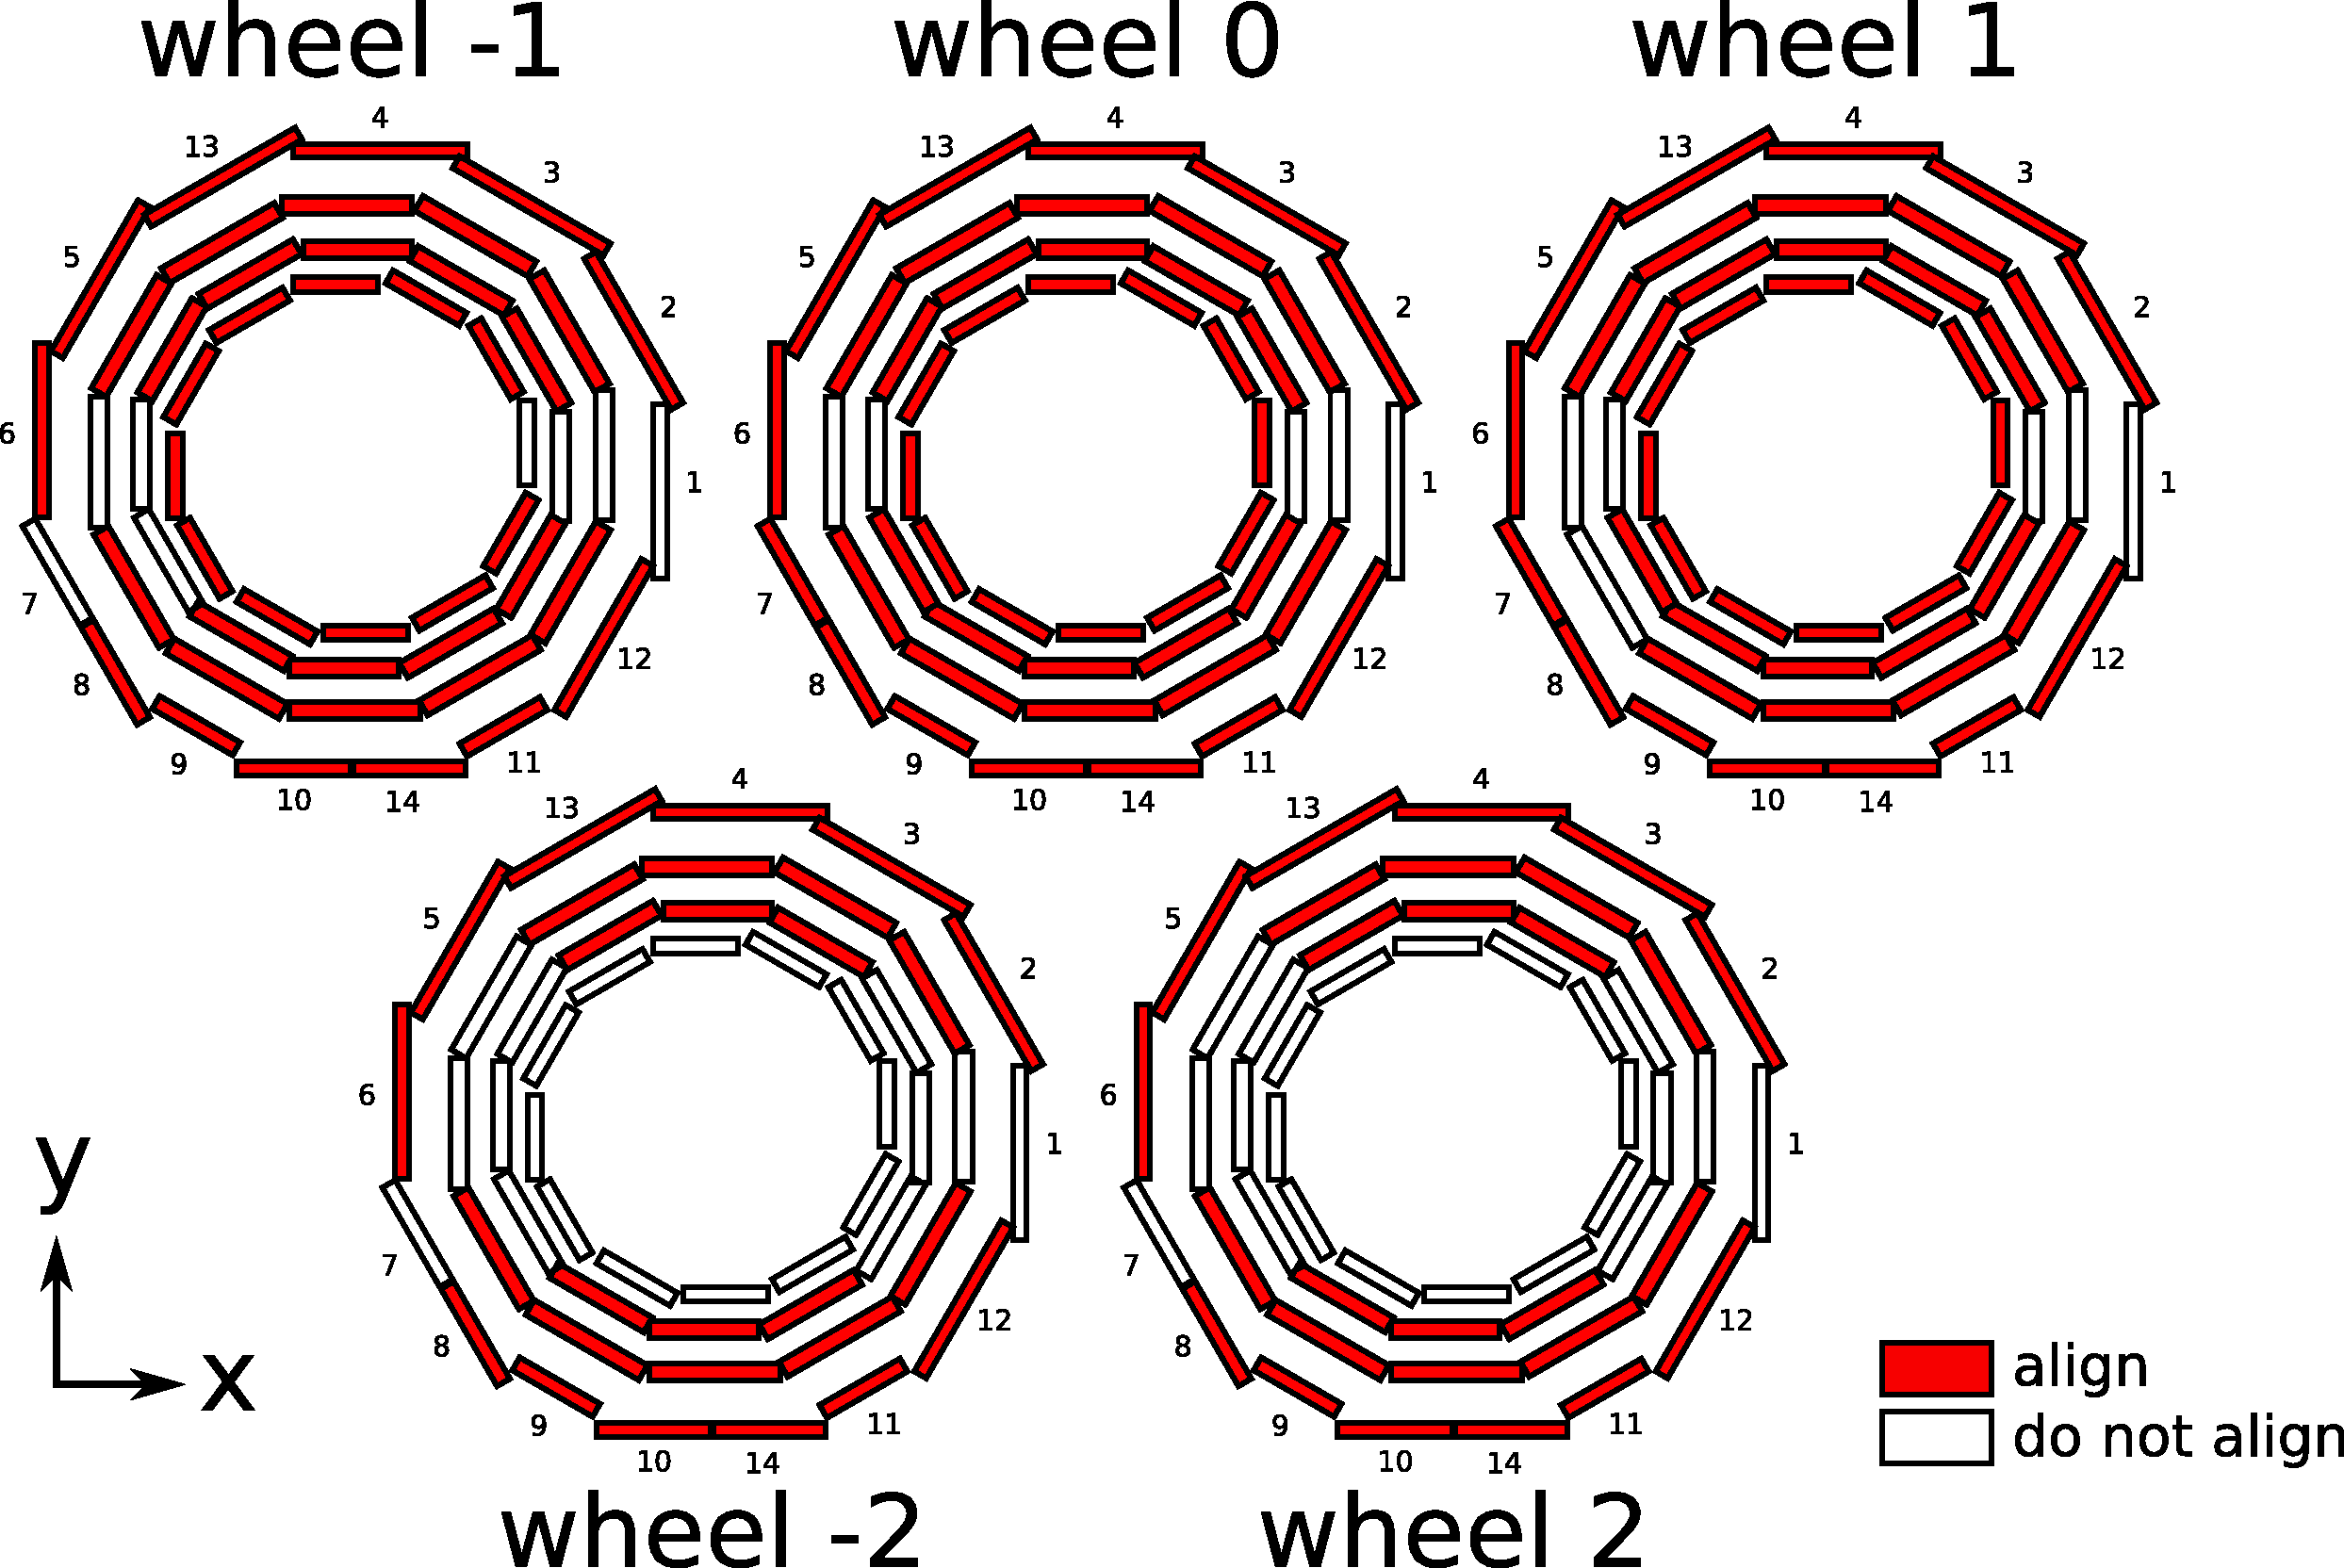
\includegraphics[width=1.1\linewidth]{data_final_map.pdf}
\column{0.5\linewidth}
\begin{itemize}
\item Chambers selected by the above shown at left
\item APE = 0 for aligned, 1000~cm for not aligned for \mbox{TrackerPointing\hspace{-0.5 cm}} $+$ SuperPointing reprocessing {\it only}
\item Distributions of aligned positions on next page
\end{itemize}
\end{columns}
\end{frame}

\begin{frame}
\frametitle{Proposal for TrackerPointing}

\begin{itemize}
\item Changes in parameter values between CRAFT\_ALL\_V11 and proposal for TrackerPointing $+$ SuperPointing skim reprocessing
\end{itemize}

\vfill
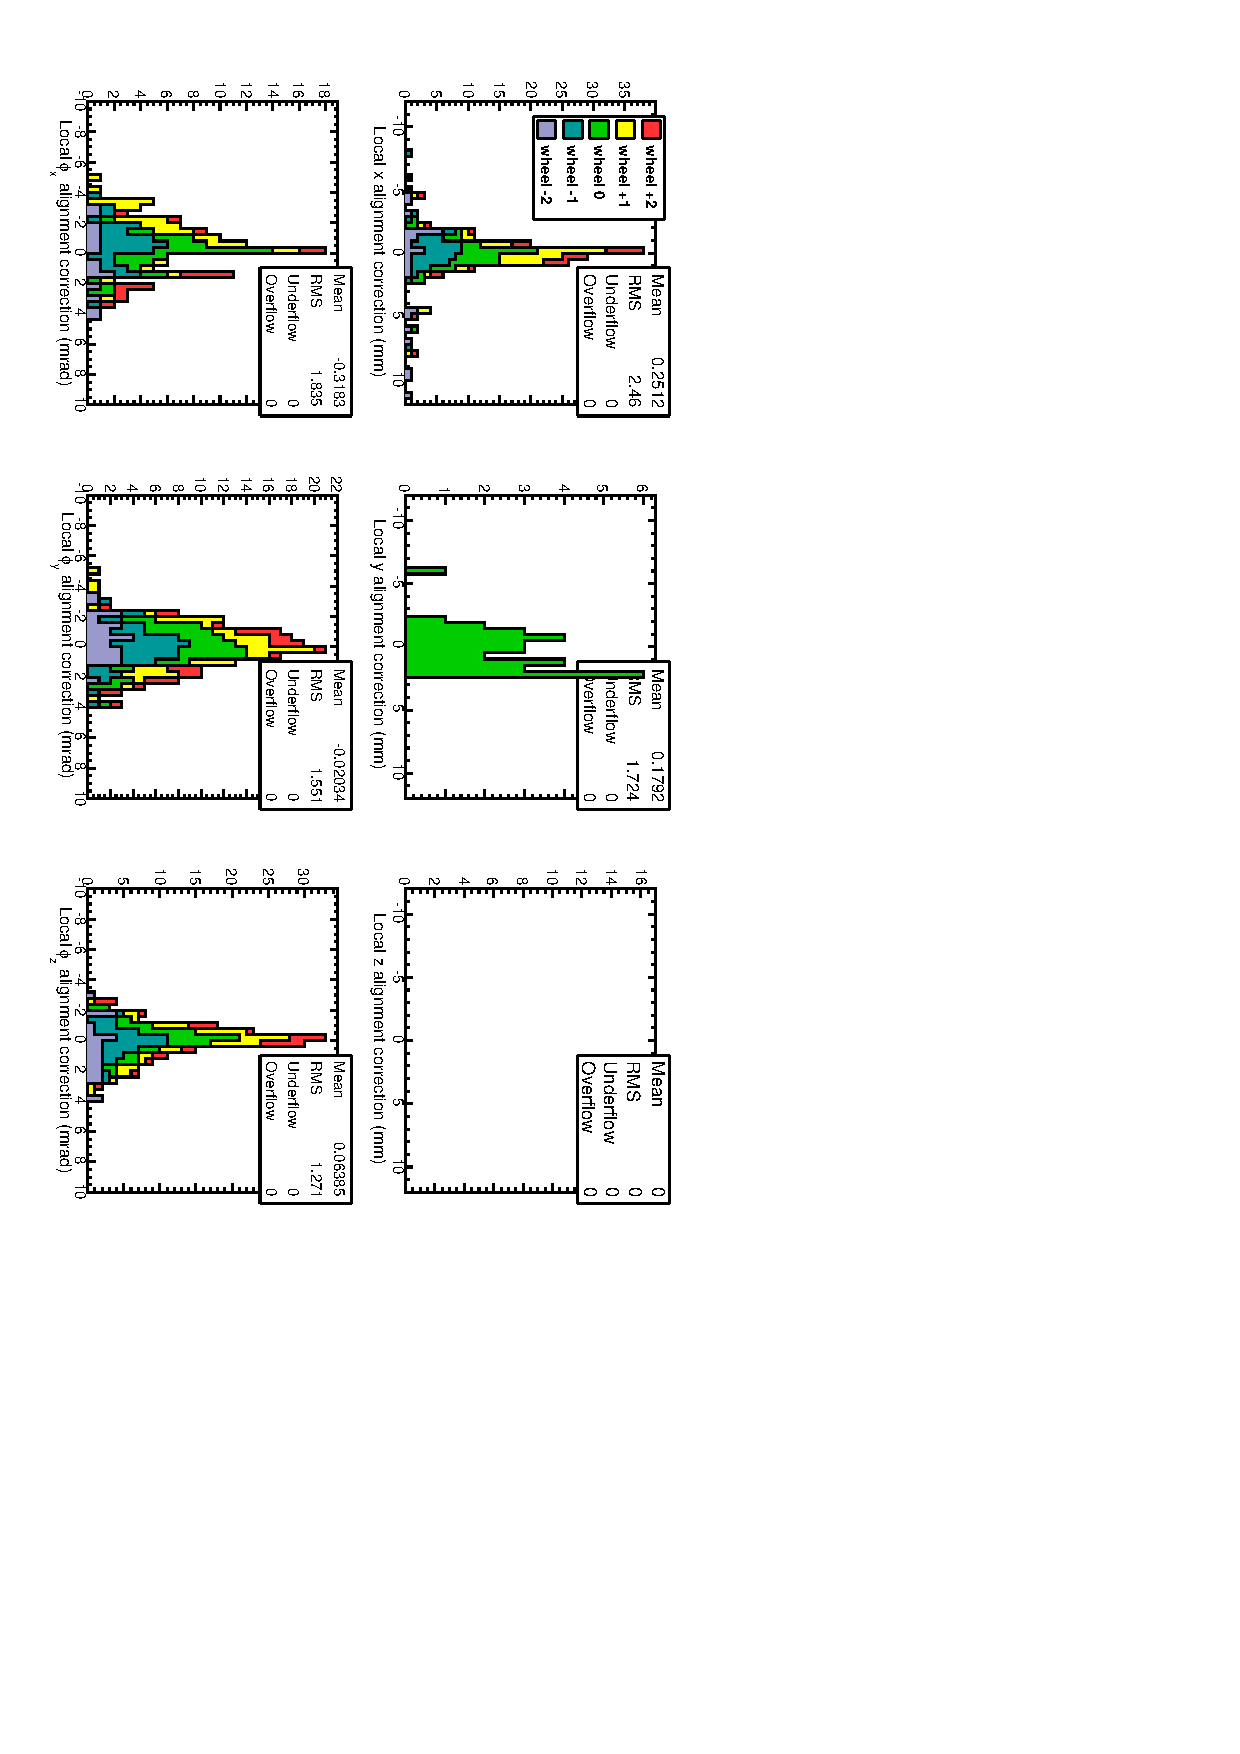
\includegraphics[height=\linewidth, angle=90]{data_final_corrections.pdf}

\vfill
{\tiny \tt /afs/cern.ch/cms/CAF/CMSALCA/ALCA\_MUONALIGN/SWAlignment/MuonAlignmentFromReference/

\hfill CMSSW\_2\_2\_7/src/final\_production\_alignment.db}
\end{frame}

\begin{frame}
\frametitle{CSC investigations}

\begin{itemize}
\item Use same alignment framework to look for large CSC displacements using globalMuons
\item Fix all parameters except $\delta_x$ due to low statistics
\end{itemize}

\begin{columns}
\column{0.5\linewidth}
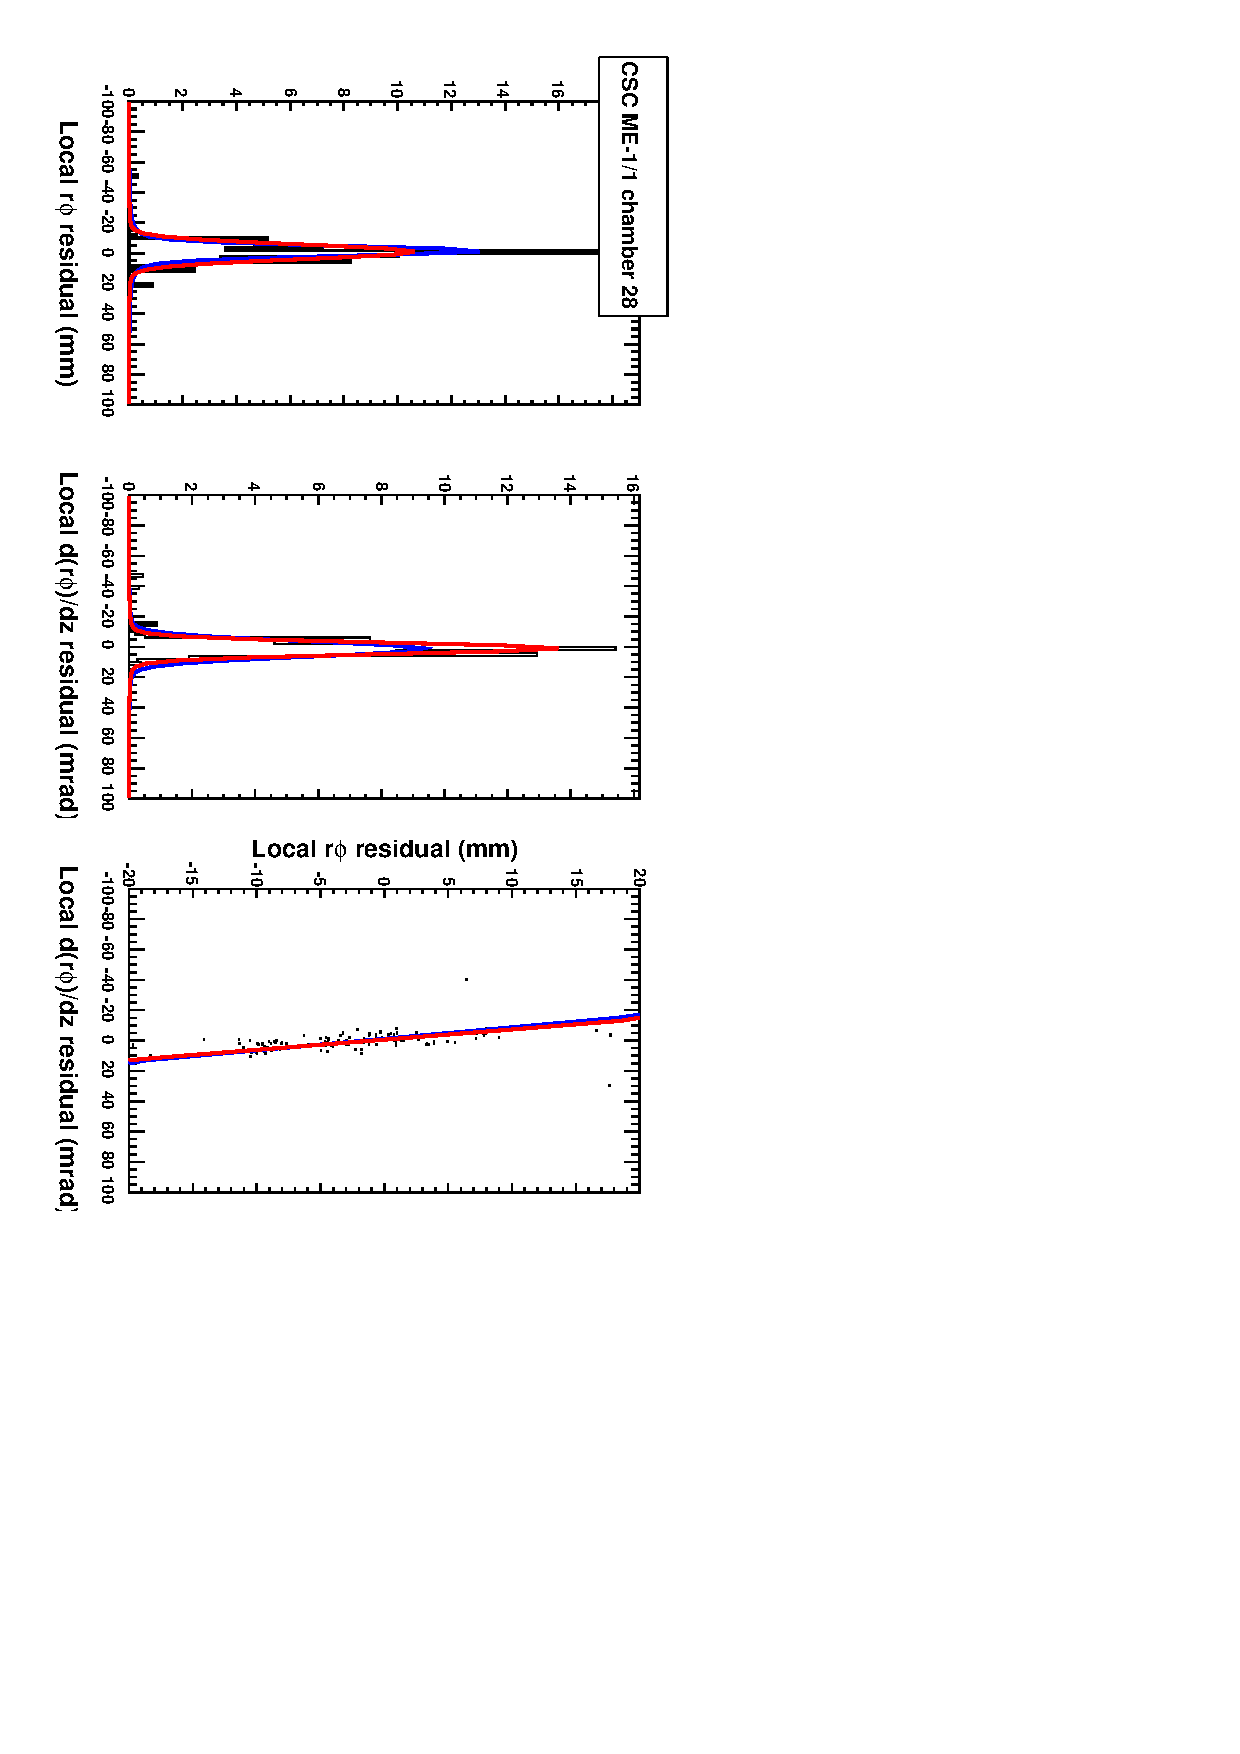
\includegraphics[height=\linewidth, angle=90]{datafit_csc_me11.pdf}

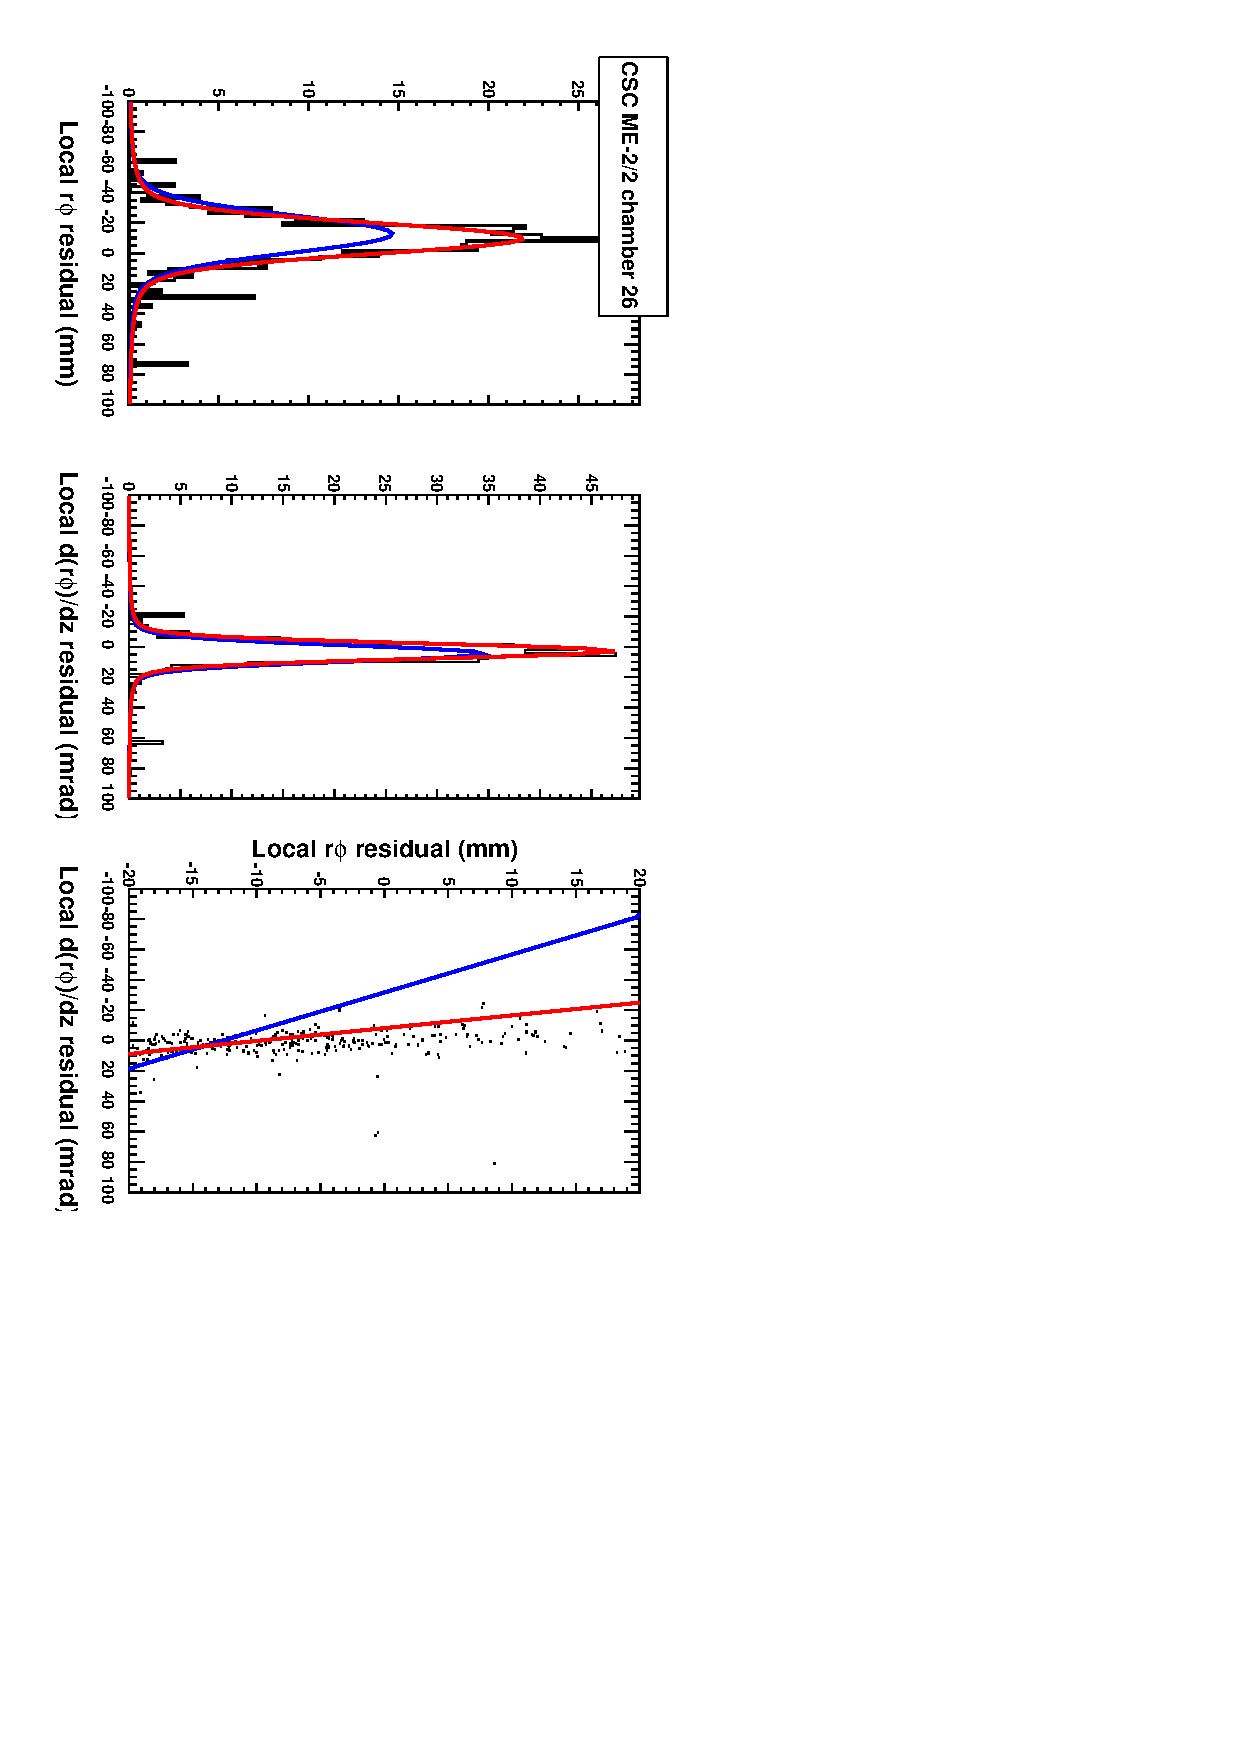
\includegraphics[height=\linewidth, angle=90]{datafit_csc_me22.pdf}

\column{0.5\linewidth}
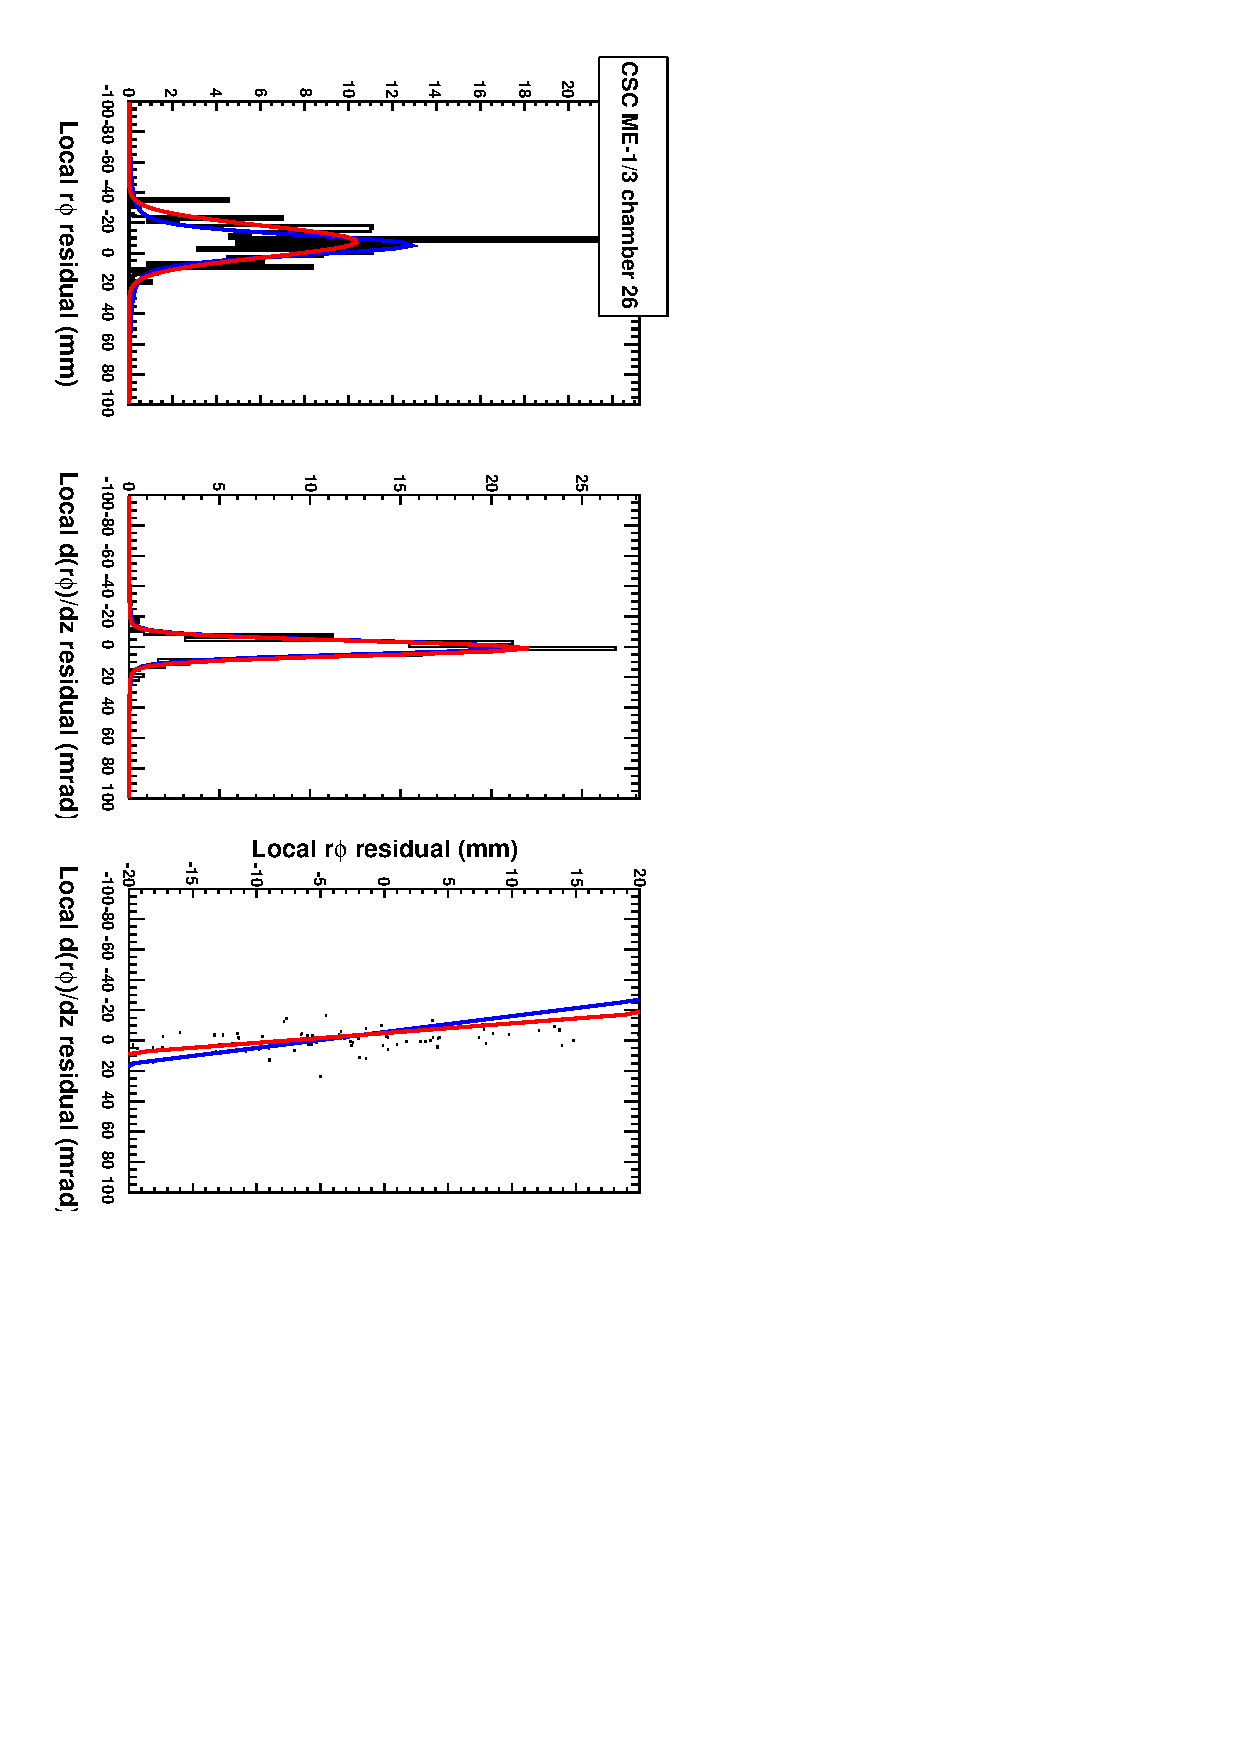
\includegraphics[height=\linewidth, angle=90]{datafit_csc_me13.pdf}

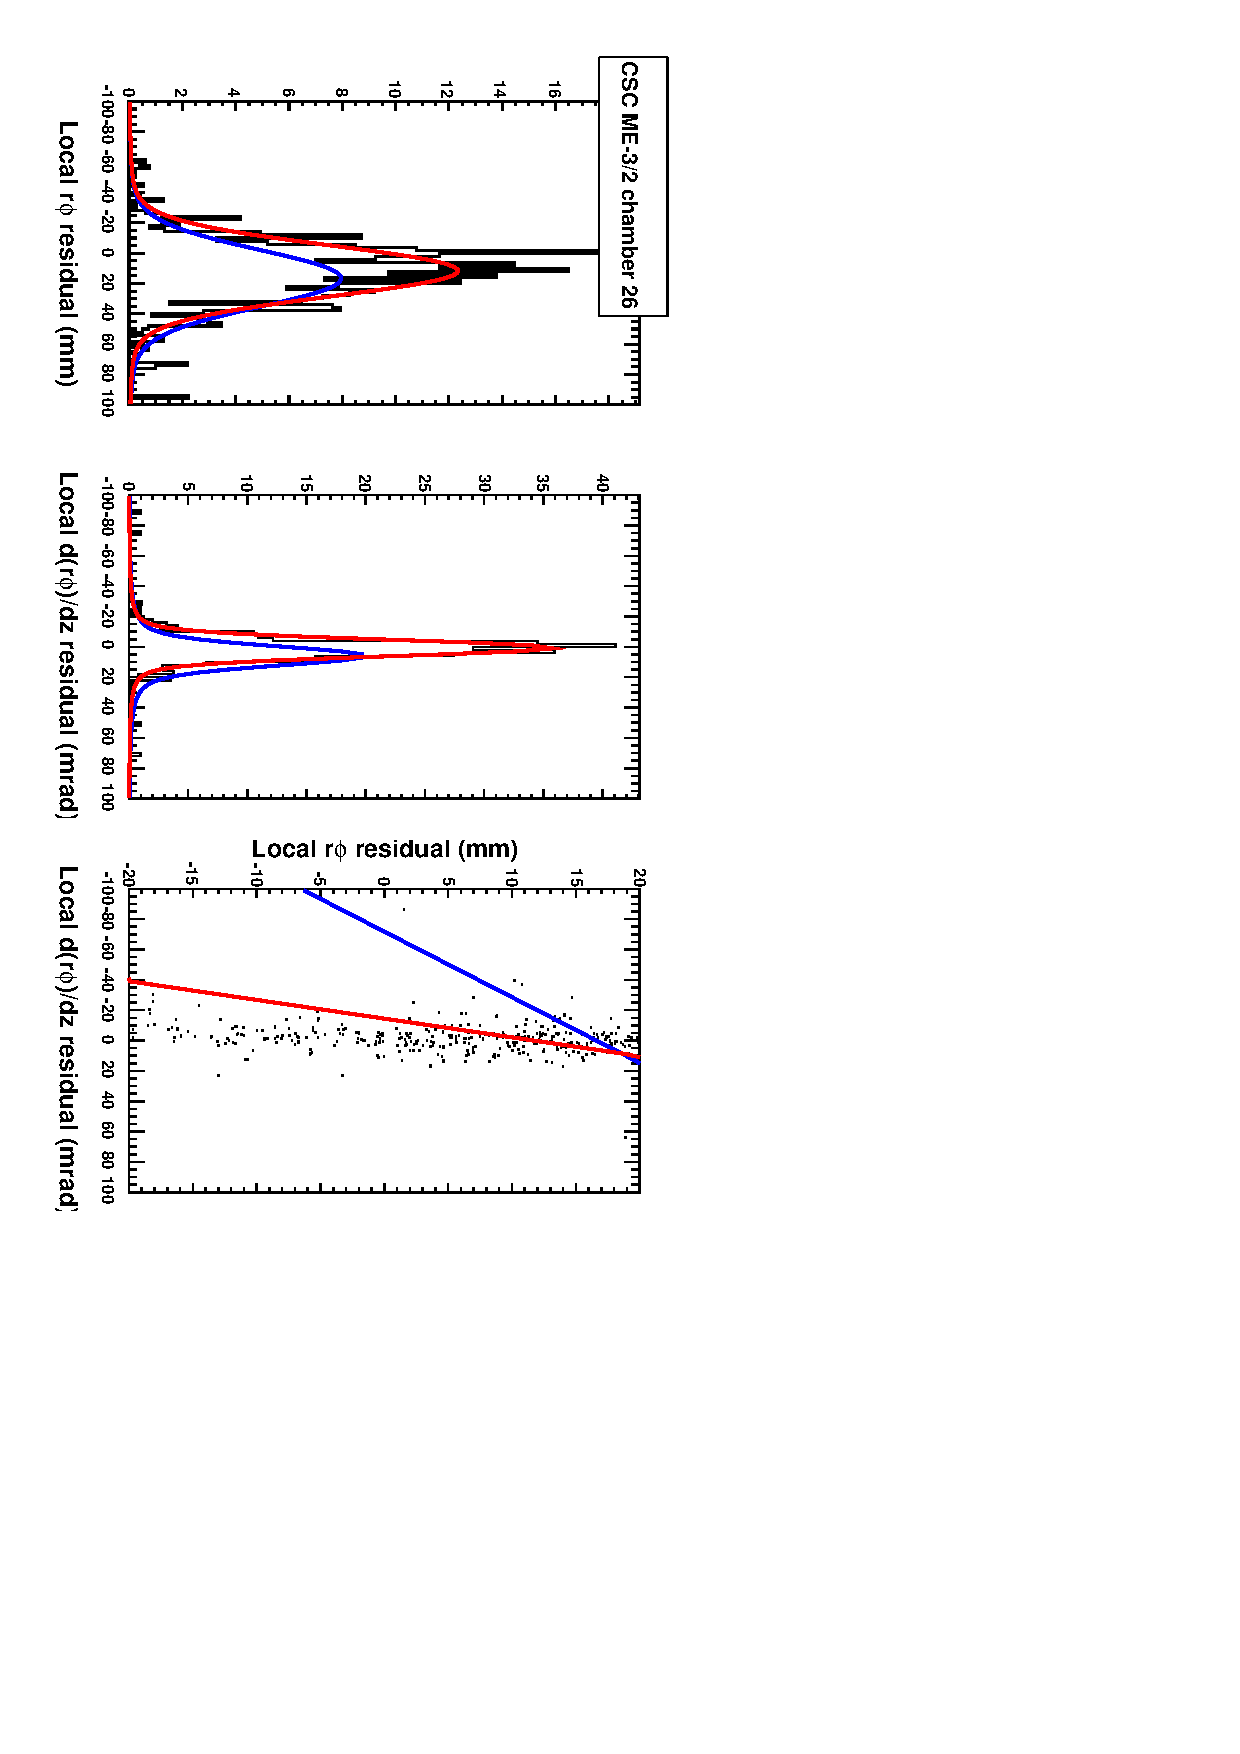
\includegraphics[height=\linewidth, angle=90]{datafit_csc_me32_agrees.pdf}
\end{columns}
\end{frame}

\begin{frame}
\frametitle{Measured CSC $r\phi$ offsets}

\begin{itemize}
\item Temporarily missing data from tops of rings \\ (probably using wrong globalMuon collection: 1-leg rather \mbox{than 2-leg)\hspace{-1 cm}}
\item Large (10~mm) collective misalignments on minus endcap
\item ME$-$2/2 agrees with ME$-$3/2, indicating disk misalignment
\end{itemize}

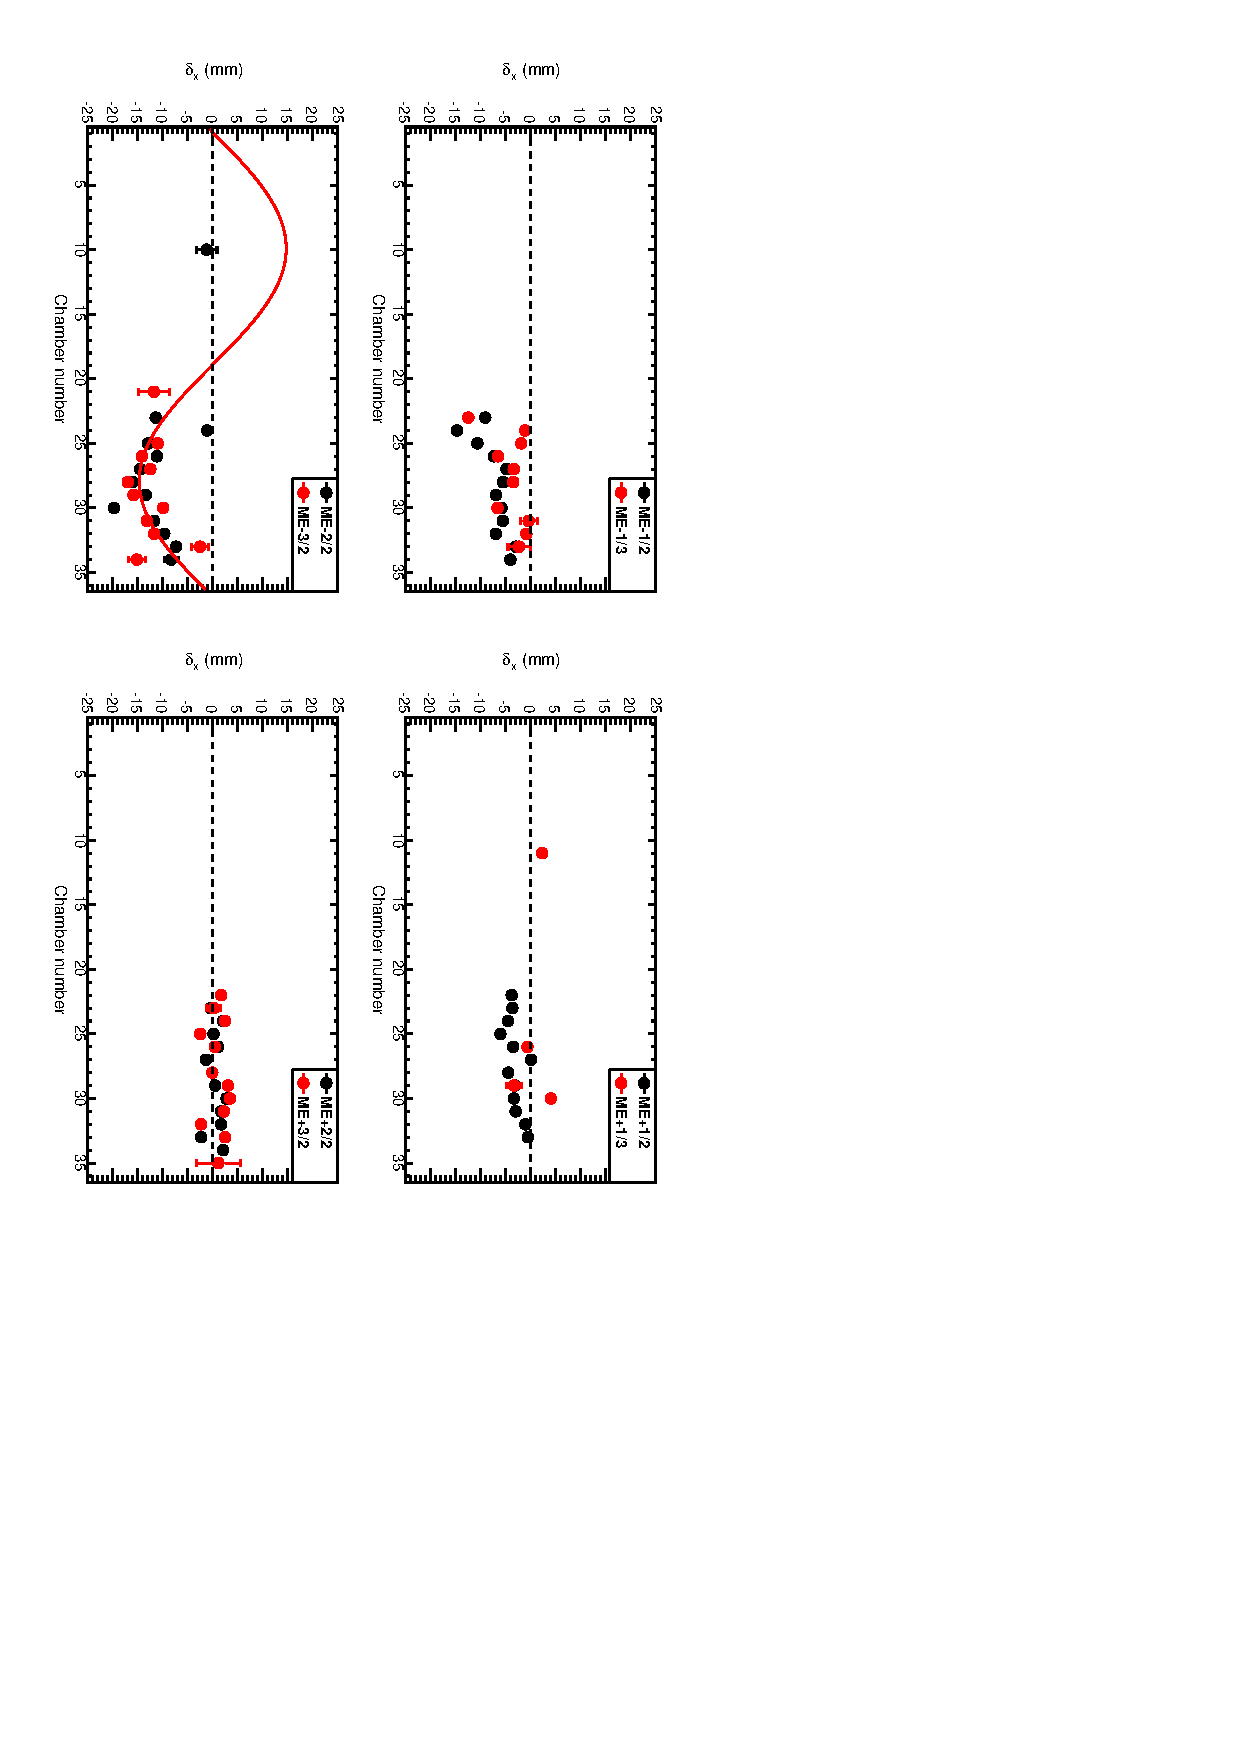
\includegraphics[height=\linewidth, angle=90]{data_endcap_alignments.pdf}
\end{frame}

\begin{frame}
\frametitle{Conclusions}
\begin{itemize}\setlength{\itemsep}{0.25 cm}
\item Techniques learned from first CRAFT alignment incorporated into
  a highly-constrained fit for 6 DOF
\begin{itemize}\setlength{\itemsep}{0.1 cm}
\item Matrix thoroughly tested, with and without measurement error
\item ``Sawtooth'' is linearly independent of alignment parameters
\item $\vec{B}(\vec{x})$ and $dE/dx$ uncertainty is degenerate with local $\delta_z$
\end{itemize}

\item More detailed plotting reveals internal DT structures in residuals

\item Fixing $\delta_z = 0$ yields a more true alignment,
  independently verified by residuals differences
\begin{itemize}\setlength{\itemsep}{0.1 cm}
\item residuals differences indicate agreement between global and local-within-sectors alignments
\item it would be very interesting to see a local-within-stations cross-check!  (DT analogy of CSC Overlaps procedure)
\end{itemize}

\item Proposed constants for TrackerPointing $+$ \mbox{SuperPointing reprocessing\hspace{-1 cm}}
\begin{itemize}
\item important updates in some parameters (especially $\phi_y$)
\end{itemize}

\item Started investigations into CSC disk misalignment
\end{itemize}
\label{numpages}
\end{frame}

%% \section*{First section}
%% \begin{frame}
%% \begin{center}
%% \Huge \textcolor{blue}{First section}
%% \end{center}
%% \end{frame}

\begin{frame}
\frametitle{Proposed constants}
\framesubtitle{local parameters relative to ideal in mm and mrad}

\tiny

Wheel -2 station 2 sector 3 $x$ -0.858923 $y$ -0.0720215 $z$ 2.80667 $\phi_x$ 3.96011 $\phi_y$ -5.33354 $\phi_z$ 2.23048 \\
Wheel -2 station 2 sector 4 $x$ 1.07277 $y$ -0.0067139 $z$ 5.97687 $\phi_x$ -0.73094 $\phi_y$ -2.1354 $\phi_z$ -0.22626 \\
Wheel -2 station 2 sector 5 $x$ 1.24524 $y$ -0.907593 $z$ 2.79189 $\phi_x$ -0.85864 $\phi_y$ 1.42262 $\phi_z$ -0.04094 \\
Wheel -2 station 2 sector 9 $x$ 2.99256 $y$ -1.89636 $z$ 1.76863 $\phi_x$ 0.54153 $\phi_y$ -0.9352 $\phi_z$ -1.05429 \\
Wheel -2 station 2 sector 10 $x$ 6.99802 $y$ -1.06567 $z$ 3.29407 $\phi_x$ -0.34119 $\phi_y$ 0.16928 $\phi_z$ 0.87478 \\
Wheel -2 station 2 sector 11 $x$ 11.3105 $y$ -1.88721 $z$ 2.62662 $\phi_x$ -2.30027 $\phi_y$ 0.23883 $\phi_z$ 1.08601 \\
Wheel -2 station 3 sector 2 $x$ 6.46888 $y$ -1.74744 $z$ -2.80803 $\phi_x$ 1.16527 $\phi_y$ -4.82761 $\phi_z$ 1.73633 \\
Wheel -2 station 3 sector 3 $x$ 3.75496 $y$ -1.37756 $z$ 1.95508 $\phi_x$ 1.6912 $\phi_y$ -3.45107 $\phi_z$ 2.58493 \\
Wheel -2 station 3 sector 4 $x$ 1.68022 $y$ 3.79272 $z$ 4.63501 $\phi_x$ 3.05403 $\phi_y$ -0.94105 $\phi_z$ 1.89042 \\
Wheel -2 station 3 sector 5 $x$ 0.54414 $y$ 1.81335 $z$ 2.62827 $\phi_x$ 4.73392 $\phi_y$ 1.37383 $\phi_z$ 0.64016 \\
Wheel -2 station 3 sector 8 $x$ 3.61984 $y$ -2.89368 $z$ -2.41129 $\phi_x$ -1.65342 $\phi_y$ -3.91324 $\phi_z$ -0.02912 \\
Wheel -2 station 3 sector 9 $x$ 5.68894 $y$ -1.99646 $z$ 3.0322 $\phi_x$ -2.74787 $\phi_y$ -1.26053 $\phi_z$ -1.43302 \\
Wheel -2 station 3 sector 10 $x$ 6.74927 $y$ 4.88831 $z$ 4.22668 $\phi_x$ 2.00942 $\phi_y$ -0.69467 $\phi_z$ 0.95828 \\
Wheel -2 station 3 sector 11 $x$ 8.60024 $y$ -1.57837 $z$ 1.75396 $\phi_x$ 0.3483 $\phi_y$ 1.73684 $\phi_z$ -0.28396 \\
Wheel -2 station 3 sector 12 $x$ 8.05289 $y$ -1.49963 $z$ -4.65297 $\phi_x$ 2.11138 $\phi_y$ 3.22851 $\phi_z$ 0.13574 \\
Wheel -2 station 4 sector 2 $x$ 9.72444 $y$ -0.511475 $z$ -5.18802 $\phi_x$ 0.51305 $\phi_y$ -3.40401 $\phi_z$ 2.43357 \\
Wheel -2 station 4 sector 3 $x$ 6.2483 $y$ -1.19995 $z$ -0.0136648 $\phi_x$ 0.41225 $\phi_y$ -3.34996 $\phi_z$ 1.30165 \\
Wheel -2 station 4 sector 4 $x$ 7.0369 $y$ -3.94897 $z$ 4.81384 $\phi_x$ 0.6729 $\phi_y$ -2.31353 $\phi_z$ 0.74123 \\
Wheel -2 station 4 sector 5 $x$ -0.524401 $y$ -0.548096 $z$ 0.5297 $\phi_x$ 0.04806 $\phi_y$ 1.22018 $\phi_z$ -0.61708 \\
Wheel -2 station 4 sector 6 $x$ -0.894128 $y$ -1.74072 $z$ -4.65677 $\phi_x$ 0.19692 $\phi_y$ 1.44744 $\phi_z$ -0.85629 \\
Wheel -2 station 4 sector 8 $x$ 3.43594 $y$ -2.00562 $z$ -2.39533 $\phi_x$ -0.66752 $\phi_y$ -1.73741 $\phi_z$ -2.39205 \\
Wheel -2 station 4 sector 9 $x$ 2.57994 $y$ -2.99194 $z$ 3.18522 $\phi_x$ -0.67428 $\phi_y$ -2.53263 $\phi_z$ -0.14228 \\
Wheel -2 station 4 sector 10 $x$ 6.97891 $y$ -3.17749 $z$ 5.5719 $\phi_x$ -0.42322 $\phi_y$ 1.23173 $\phi_z$ -1.87454 \\
Wheel -2 station 4 sector 11 $x$ 6.34256 $y$ -1.29089 $z$ 2.13981 $\phi_x$ 0.98053 $\phi_y$ 1.26424 $\phi_z$ 1.2012 \\
Wheel -2 station 4 sector 12 $x$ 6.41509 $y$ -0.737305 $z$ -3.53497 $\phi_x$ 0.32122 $\phi_y$ 1.88682 $\phi_z$ 1.25792 \\
Wheel -2 station 4 sector 13 $x$ 1.78986 $y$ -2.51648 $z$ 4.39148 $\phi_x$ -0.15294 $\phi_y$ 1.69593 $\phi_z$ -2.43774 \\
Wheel -2 station 4 sector 14 $x$ 7.5322 $y$ -1.58081 $z$ 4.97314 $\phi_x$ 0.32806 $\phi_y$ 0.92582 $\phi_z$ 0.93819 \\
Wheel -1 station 1 sector 2 $x$ 0.851181 $y$ -1.26953 $z$ -3.52266 $\phi_x$ 2.13109 $\phi_y$ -4.03852 $\phi_z$ -0.18744 \\
Wheel -1 station 1 sector 3 $x$ 1.69849 $y$ -0.015564 $z$ 2.10756 $\phi_x$ -0.15521 $\phi_y$ -3.26974 $\phi_z$ -0.33618 \\
Wheel -1 station 1 sector 4 $x$ 1.23409 $y$ 1.93726 $z$ 4.89441 $\phi_x$ 2.22465 $\phi_y$ 0.14531 $\phi_z$ -0.13689 \\
Wheel -1 station 1 sector 5 $x$ 3.94354 $y$ 1.77826 $z$ 1.78128 $\phi_x$ -0.7791 $\phi_y$ 3.34266 $\phi_z$ -2.14837 \\
Wheel -1 station 1 sector 6 $x$ 1.06901 $y$ -1.24908 $z$ -2.93099 $\phi_x$ -0.02112 $\phi_y$ 5.47121 $\phi_z$ 0.09473 \\

\end{frame}

\begin{frame}
\frametitle{Proposed constants}
\framesubtitle{local parameters relative to ideal in mm and mrad}

\tiny

Wheel -1 station 1 sector 7 $x$ 2.58514 $y$ 1.96991 $z$ -4.85504 $\phi_x$ -1.14318 $\phi_y$ 1.7261 $\phi_z$ -0.6607 \\
Wheel -1 station 1 sector 8 $x$ 1.14522 $y$ 1.38611 $z$ -3.36188 $\phi_x$ 0.41927 $\phi_y$ -1.93849 $\phi_z$ -2.0445 \\
Wheel -1 station 1 sector 9 $x$ 0.684911 $y$ 0.18158 $z$ 1.8441 $\phi_x$ 0.10399 $\phi_y$ -1.81308 $\phi_z$ -1.31284 \\
Wheel -1 station 1 sector 10 $x$ 2.42973 $y$ 0.242615 $z$ 5.30792 $\phi_x$ 1.67733 $\phi_y$ 1.11036 $\phi_z$ 0.23085 \\
Wheel -1 station 1 sector 11 $x$ 6.65886 $y$ -2.7948 $z$ 0.944794 $\phi_x$ -0.93816 $\phi_y$ 2.54819 $\phi_z$ 0.53715 \\
Wheel -1 station 1 sector 12 $x$ 6.07349 $y$ 0.561218 $z$ -3.90522 $\phi_x$ 0.98034 $\phi_y$ 1.33822 $\phi_z$ 1.40098 \\
Wheel -1 station 2 sector 2 $x$ 1.27805 $y$ 0.910645 $z$ -4.53837 $\phi_x$ -1.33999 $\phi_y$ -4.87714 $\phi_z$ 2.26321 \\
Wheel -1 station 2 sector 3 $x$ 2.00527 $y$ -0.811462 $z$ 0.78703 $\phi_x$ -4.21608 $\phi_y$ -3.29525 $\phi_z$ -0.1112 \\
Wheel -1 station 2 sector 4 $x$ 0.812187 $y$ 1.0321 $z$ 3.75244 $\phi_x$ -1.88002 $\phi_y$ -1.2377 $\phi_z$ -0.03208 \\
Wheel -1 station 2 sector 5 $x$ 0.984457 $y$ -0.551148 $z$ 1.61113 $\phi_x$ -1.91649 $\phi_y$ 2.71483 $\phi_z$ 0.40509 \\
Wheel -1 station 2 sector 6 $x$ -0.0057912 $y$ -4.08295 $z$ -3.85105 $\phi_x$ -2.83985 $\phi_y$ 4.13584 $\phi_z$ -1.16917 \\
Wheel -1 station 2 sector 9 $x$ 0.232805 $y$ -1.28174 $z$ 0.813811 $\phi_x$ -2.69568 $\phi_y$ -1.32692 $\phi_z$ -0.30736 \\
Wheel -1 station 2 sector 10 $x$ 2.01275 $y$ -0.827332 $z$ 4.96704 $\phi_x$ -1.04391 $\phi_y$ 1.34498 $\phi_z$ -0.16109 \\
Wheel -1 station 2 sector 11 $x$ 5.8136 $y$ -4.02344 $z$ 1.29748 $\phi_x$ -2.6418 $\phi_y$ 2.68797 $\phi_z$ -0.19522 \\
Wheel -1 station 2 sector 12 $x$ 4.37855 $y$ -1.26282 $z$ -4.59131 $\phi_x$ -2.01649 $\phi_y$ 2.35011 $\phi_z$ 0.83574 \\
Wheel -1 station 3 sector 2 $x$ 5.14254 $y$ 0.671692 $z$ -4.35886 $\phi_x$ -0.05725 $\phi_y$ -2.38851 $\phi_z$ -0.65212 \\
Wheel -1 station 3 sector 3 $x$ 3.83586 $y$ -1.32812 $z$ 1.21315 $\phi_x$ -0.47087 $\phi_y$ -2.42001 $\phi_z$ -0.02429 \\
Wheel -1 station 3 sector 4 $x$ 1.80733 $y$ 2.37885 $z$ 2.8186 $\phi_x$ 3.57361 $\phi_y$ -0.78949 $\phi_z$ 0.019 \\
Wheel -1 station 3 sector 5 $x$ -0.630927 $y$ 0.423889 $z$ 1.61594 $\phi_x$ -0.39316 $\phi_y$ 1.69806 $\phi_z$ 1.55537 \\
Wheel -1 station 3 sector 6 $x$ 1.29171 $y$ -2.85614 $z$ -3.89869 $\phi_x$ -0.32836 $\phi_y$ 3.4787 $\phi_z$ 0.21418 \\
Wheel -1 station 3 sector 8 $x$ 2.07733 $y$ -0.0100708 $z$ -3.71398 $\phi_x$ 0.80849 $\phi_y$ -2.47492 $\phi_z$ -1.88791 \\
Wheel -1 station 3 sector 9 $x$ 1.00799 $y$ -1.3443 $z$ 2.31782 $\phi_x$ -0.75375 $\phi_y$ -2.88205 $\phi_z$ -1.00432 \\
Wheel -1 station 3 sector 10 $x$ 1.24508 $y$ 2.82745 $z$ 5.31433 $\phi_x$ 0.89432 $\phi_y$ 0.09742 $\phi_z$ 0.38588 \\
Wheel -1 station 3 sector 11 $x$ 3.80897 $y$ -2.79053 $z$ 1.81034 $\phi_x$ -0.80268 $\phi_y$ 1.85814 $\phi_z$ -0.45142 \\
Wheel -1 station 3 sector 12 $x$ 3.38981 $y$ -1.48163 $z$ -4.60363 $\phi_x$ -0.12083 $\phi_y$ 2.18909 $\phi_z$ 1.23862 \\
Wheel -1 station 4 sector 2 $x$ 6.8624 $y$ -0.81543 $z$ -5.06709 $\phi_x$ -0.34134 $\phi_y$ -0.74481 $\phi_z$ -1.7839 \\
Wheel -1 station 4 sector 3 $x$ 7.76991 $y$ -0.256043 $z$ -1.25512 $\phi_x$ -0.39782 $\phi_y$ -2.53869 $\phi_z$ 1.02988 \\
Wheel -1 station 4 sector 4 $x$ 4.2952 $y$ 0.0436401 $z$ 1.88538 $\phi_x$ 0.19289 $\phi_y$ -0.54105 $\phi_z$ 2.08803 \\
Wheel -1 station 4 sector 5 $x$ -1.02414 $y$ -0.666199 $z$ 1.04657 $\phi_x$ 1.0394 $\phi_y$ 1.99977 $\phi_z$ -1.31932 \\
Wheel -1 station 4 sector 6 $x$ -4.2617 $y$ -1.4621 $z$ -4.54662 $\phi_x$ -0.08118 $\phi_y$ 2.46445 $\phi_z$ -2.27855 \\
Wheel -1 station 4 sector 8 $x$ -0.0615974 $y$ -2.54364 $z$ -3.70044 $\phi_x$ -1.0352 $\phi_y$ -0.18402 $\phi_z$ -1.04923 \\
Wheel -1 station 4 sector 9 $x$ 0.331674 $y$ 0.214539 $z$ 1.68138 $\phi_x$ -1.04893 $\phi_y$ -1.34946 $\phi_z$ -0.92164 \\

\end{frame}

\begin{frame}
\frametitle{Proposed constants}
\framesubtitle{local parameters relative to ideal in mm and mrad}

\tiny

Wheel -1 station 4 sector 10 $x$ -1.40884 $y$ 1.0553 $z$ 4.22424 $\phi_x$ -0.9327 $\phi_y$ 0.3924 $\phi_z$ 0.43537 \\
Wheel -1 station 4 sector 11 $x$ 3.61883 $y$ -0.733948 $z$ 2.13226 $\phi_x$ 0.27058 $\phi_y$ 2.7407 $\phi_z$ 0.24152 \\
Wheel -1 station 4 sector 12 $x$ 2.03445 $y$ -1.96838 $z$ -2.3232 $\phi_x$ -0.03391 $\phi_y$ -0.02276 $\phi_z$ 2.8036 \\
Wheel -1 station 4 sector 13 $x$ 1.65863 $y$ -1.06781 $z$ 2.9071 $\phi_x$ -0.22036 $\phi_y$ 1.35953 $\phi_z$ 0.87837 \\
Wheel -1 station 4 sector 14 $x$ 1.1969 $y$ 1.59119 $z$ 5.27954 $\phi_x$ 0.18895 $\phi_y$ -0.24893 $\phi_z$ 1.64755 \\
Wheel 0 station 1 sector 1 $x$ 4.31149 $y$ -0.244357 $z$ -8.48053 $\phi_x$ 0.99252 $\phi_y$ 0.91948 $\phi_z$ -0.65497 \\
Wheel 0 station 1 sector 2 $x$ 1.11441 $y$ 3.33206 $z$ -2.19542 $\phi_x$ 1.28161 $\phi_y$ 6.25448 $\phi_z$ 1.59838 \\
Wheel 0 station 1 sector 3 $x$ 0.79053 $y$ 2.52988 $z$ 5.85166 $\phi_x$ -0.44511 $\phi_y$ 4.41379 $\phi_z$ -0.9004 \\
Wheel 0 station 1 sector 4 $x$ 0.852737 $y$ -5.83083 $z$ 8.48877 $\phi_x$ 0.563 $\phi_y$ 1.04017 $\phi_z$ 0.13207 \\
Wheel 0 station 1 sector 5 $x$ 2.21733 $y$ 1.29413 $z$ 5.03072 $\phi_x$ 0.81484 $\phi_y$ 4.1282 $\phi_z$ -0.56564 \\
Wheel 0 station 1 sector 6 $x$ -1.11174 $y$ 0.996257 $z$ -4.33983 $\phi_x$ -0.72122 $\phi_y$ -4.44425 $\phi_z$ -1.24608 \\
Wheel 0 station 1 sector 7 $x$ -0.7127 $y$ -1.87665 $z$ -8.55133 $\phi_x$ -1.14117 $\phi_y$ -0.93658 $\phi_z$ -2.47521 \\
Wheel 0 station 1 sector 8 $x$ -3.43098 $y$ -2.5747 $z$ -6.654 $\phi_x$ 0.03518 $\phi_y$ -3.81879 $\phi_z$ -2.29433 \\
Wheel 0 station 1 sector 9 $x$ -2.2637 $y$ -1.40539 $z$ 3.211 $\phi_x$ 0.44219 $\phi_y$ -4.0168 $\phi_z$ -0.92233 \\
Wheel 0 station 1 sector 10 $x$ -3.33191 $y$ 3.90959 $z$ 5.45807 $\phi_x$ 1.33823 $\phi_y$ 1.06359 $\phi_z$ -1.20489 \\
Wheel 0 station 1 sector 11 $x$ -6.04528 $y$ 2.21034 $z$ 3.50357 $\phi_x$ 0.37176 $\phi_y$ -4.15583 $\phi_z$ -0.38046 \\
Wheel 0 station 1 sector 12 $x$ 10.62 $y$ -1.01235 $z$ -7.82866 $\phi_x$ -0.69138 $\phi_y$ 3.98762 $\phi_z$ -1.12286 \\
Wheel 0 station 2 sector 2 $x$ 1.62126 $y$ 2.28219 $z$ -4.72858 $\phi_x$ -0.56968 $\phi_y$ 1.23423 $\phi_z$ -0.29783 \\
Wheel 0 station 2 sector 3 $x$ -0.806553 $y$ -0.295698 $z$ 4.61924 $\phi_x$ -1.34884 $\phi_y$ 3.50955 $\phi_z$ 2.13239 \\
Wheel 0 station 2 sector 4 $x$ 2.30427 $y$ -8.14645 $z$ 8.60016 $\phi_x$ -0.29633 $\phi_y$ -2.72441 $\phi_z$ 0.60622 \\
Wheel 0 station 2 sector 5 $x$ 1.57191 $y$ 1.3299 $z$ 5.73776 $\phi_x$ 0.2668 $\phi_y$ 3.14588 $\phi_z$ 1.18292 \\
Wheel 0 station 2 sector 6 $x$ 0.545702 $y$ 0.507466 $z$ -1.7306 $\phi_x$ -2.77717 $\phi_y$ -4.33322 $\phi_z$ 0.45867 \\
Wheel 0 station 2 sector 8 $x$ -2.44087 $y$ -2.09158 $z$ -5.63427 $\phi_x$ -0.00477 $\phi_y$ -3.31363 $\phi_z$ -1.63931 \\
Wheel 0 station 2 sector 9 $x$ -2.11484 $y$ 0.31826 $z$ 2.36418 $\phi_x$ 0.31905 $\phi_y$ -3.04983 $\phi_z$ -0.22975 \\
Wheel 0 station 2 sector 10 $x$ 0.617771 $y$ 4.44215 $z$ 6.6571 $\phi_x$ -1.39624 $\phi_y$ -0.30562 $\phi_z$ 0.08301 \\
Wheel 0 station 2 sector 11 $x$ -3.27321 $y$ 3.59291 $z$ 3.29205 $\phi_x$ -0.61194 $\phi_y$ -5.16856 $\phi_z$ 1.2275 \\
Wheel 0 station 2 sector 12 $x$ 9.83251 $y$ -1.23156 $z$ -6.55066 $\phi_x$ -0.29319 $\phi_y$ 3.39463 $\phi_z$ 1.20365 \\
Wheel 0 station 3 sector 2 $x$ -1.58877 $y$ 1.71524 $z$ -4.20434 $\phi_x$ 0.96071 $\phi_y$ 4.64165 $\phi_z$ 0.86643 \\
Wheel 0 station 3 sector 3 $x$ -3.78264 $y$ 0.422799 $z$ 5.03824 $\phi_x$ 2.61095 $\phi_y$ 4.18387 $\phi_z$ 0.26061 \\
Wheel 0 station 3 sector 4 $x$ 2.31722 $y$ -4.15166 $z$ 10.249 $\phi_x$ -1.54944 $\phi_y$ 0.00255 $\phi_z$ -0.13908 \\
Wheel 0 station 3 sector 5 $x$ -0.571674 $y$ 3.78601 $z$ 6.31147 $\phi_x$ -0.53773 $\phi_y$ 3.35972 $\phi_z$ 0.28602 \\
Wheel 0 station 3 sector 6 $x$ 2.56187 $y$ -1.83215 $z$ -3.42709 $\phi_x$ -0.3067 $\phi_y$ -4.04527 $\phi_z$ -0.8713 \\

\end{frame}

\begin{frame}
\frametitle{Proposed constants}
\framesubtitle{local parameters relative to ideal in mm and mrad}

\tiny

Wheel 0 station 3 sector 8 $x$ -2.60014 $y$ -1.15745 $z$ -4.88687 $\phi_x$ 0.32136 $\phi_y$ -3.32985 $\phi_z$ -1.43223 \\
Wheel 0 station 3 sector 9 $x$ -1.30916 $y$ -0.481679 $z$ 3.21908 $\phi_x$ 0.21335 $\phi_y$ -2.136 $\phi_z$ -0.00664 \\
Wheel 0 station 3 sector 10 $x$ -1.49691 $y$ 4.14856 $z$ 7.38953 $\phi_x$ 2.56641 $\phi_y$ -0.00575 $\phi_z$ -0.39747 \\
Wheel 0 station 3 sector 11 $x$ -5.05493 $y$ 3.50028 $z$ 4.06302 $\phi_x$ -0.19602 $\phi_y$ -3.61992 $\phi_z$ -0.65023 \\
Wheel 0 station 3 sector 12 $x$ 9.75095 $y$ -3.44321 $z$ -5.95042 $\phi_x$ 1.1613 $\phi_y$ 2.58857 $\phi_z$ 0.40561 \\
Wheel 0 station 4 sector 2 $x$ -2.79989 $y$ -0.482284 $z$ -6.35894 $\phi_x$ -0.53711 $\phi_y$ 1.71273 $\phi_z$ -1.06504 \\
Wheel 0 station 4 sector 3 $x$ -6.40613 $y$ 1.36144 $z$ 1.52083 $\phi_x$ -0.1756 $\phi_y$ 3.65436 $\phi_z$ -0.52607 \\
Wheel 0 station 4 sector 4 $x$ 6.8457 $y$ 0.153022 $z$ 6.59851 $\phi_x$ 0.07554 $\phi_y$ -1.62017 $\phi_z$ 1.00673 \\
Wheel 0 station 4 sector 5 $x$ -2.47676 $y$ 0.612476 $z$ 4.85868 $\phi_x$ -0.08818 $\phi_y$ 3.87655 $\phi_z$ 0.03601 \\
Wheel 0 station 4 sector 6 $x$ 3.40954 $y$ 1.25147 $z$ -4.89895 $\phi_x$ -0.69604 $\phi_y$ -2.47187 $\phi_z$ -1.23236 \\
Wheel 0 station 4 sector 7 $x$ 1.40625 $y$ 0.402119 $z$ -8.11646 $\phi_x$ -0.18864 $\phi_y$ -0.28251 $\phi_z$ -0.13526 \\
Wheel 0 station 4 sector 8 $x$ -2.55356 $y$ 1.1972 $z$ -9.71891 $\phi_x$ -0.14007 $\phi_y$ 2.22931 $\phi_z$ -2.11928 \\
Wheel 0 station 4 sector 9 $x$ -2.20721 $y$ -2.96517 $z$ 4.94177 $\phi_x$ 0.05375 $\phi_y$ -2.93942 $\phi_z$ -0.99161 \\
Wheel 0 station 4 sector 10 $x$ 0.687561 $y$ 1.21544 $z$ 7.98645 $\phi_x$ -0.73872 $\phi_y$ 0.96927 $\phi_z$ 0.00373 \\
Wheel 0 station 4 sector 11 $x$ -2.70243 $y$ 1.25618 $z$ 4.84614 $\phi_x$ 0.61865 $\phi_y$ -3.79912 $\phi_z$ -0.6001 \\
Wheel 0 station 4 sector 12 $x$ 8.84109 $y$ -0.139828 $z$ -5.10142 $\phi_x$ 1.3117 $\phi_y$ 0.2933 $\phi_z$ -1.47789 \\
Wheel 0 station 4 sector 13 $x$ 1.96198 $y$ 1.15505 $z$ 6.87988 $\phi_x$ -0.15212 $\phi_y$ 0.57321 $\phi_z$ -0.69774 \\
Wheel 0 station 4 sector 14 $x$ -1.85883 $y$ -0.614842 $z$ 3.33862 $\phi_x$ -0.2608 $\phi_y$ -4.84295 $\phi_z$ -2.39709 \\
Wheel 1 station 1 sector 1 $x$ -2.58495 $y$ -1.6925 $z$ -5.99884 $\phi_x$ -1.9484 $\phi_y$ -0.56512 $\phi_z$ -0.05504 \\
Wheel 1 station 1 sector 2 $x$ 0.130108 $y$ -0.216064 $z$ -3.40223 $\phi_x$ 1.62371 $\phi_y$ 4.87149 $\phi_z$ -2.1568 \\
Wheel 1 station 1 sector 3 $x$ 1.24372 $y$ -1.65558 $z$ 2.94429 $\phi_x$ -2.3927 $\phi_y$ 2.98929 $\phi_z$ -1.49108 \\
Wheel 1 station 1 sector 4 $x$ -0.840034 $y$ -0.657349 $z$ 5.87891 $\phi_x$ -1.87183 $\phi_y$ 0.26802 $\phi_z$ -0.59566 \\
Wheel 1 station 1 sector 5 $x$ -1.01297 $y$ -4.39575 $z$ 2.43018 $\phi_x$ -0.40417 $\phi_y$ -2.51583 $\phi_z$ 0.45195 \\
Wheel 1 station 1 sector 6 $x$ 1.83001 $y$ -2.36725 $z$ -3.0486 $\phi_x$ 0.08558 $\phi_y$ -3.33404 $\phi_z$ -0.26003 \\
Wheel 1 station 1 sector 7 $x$ 4.69452 $y$ -2.276 $z$ -6.70288 $\phi_x$ 1.17097 $\phi_y$ -3.28029 $\phi_z$ 0.83038 \\
Wheel 1 station 1 sector 8 $x$ 5.45029 $y$ -0.971375 $z$ -3.36291 $\phi_x$ -0.21555 $\phi_y$ 1.48713 $\phi_z$ 0.22603 \\
Wheel 1 station 1 sector 9 $x$ 2.87232 $y$ 0.239258 $z$ 2.76553 $\phi_x$ -0.74411 $\phi_y$ 3.85255 $\phi_z$ -0.03942 \\
Wheel 1 station 1 sector 10 $x$ -0.614929 $y$ 1.82465 $z$ 4.61243 $\phi_x$ -0.92573 $\phi_y$ 0.68658 $\phi_z$ 1.38139 \\
Wheel 1 station 1 sector 11 $x$ -5.79432 $y$ 1.41632 $z$ 2.28367 $\phi_x$ -1.76968 $\phi_y$ -1.41843 $\phi_z$ -0.1892 \\
Wheel 1 station 1 sector 12 $x$ -8.20031 $y$ -1.75873 $z$ -4.34373 $\phi_x$ 0.12695 $\phi_y$ -1.34722 $\phi_z$ 0.04941 \\
Wheel 1 station 2 sector 2 $x$ -0.770293 $y$ -3.03314 $z$ -3.3646 $\phi_x$ -3.42128 $\phi_y$ 2.04586 $\phi_z$ 1.27777 \\
Wheel 1 station 2 sector 3 $x$ -0.736401 $y$ -1.51642 $z$ 2.02042 $\phi_x$ -3.47135 $\phi_y$ 1.7259 $\phi_z$ 1.26397 \\

\end{frame}

\begin{frame}
\frametitle{Proposed constants}
\framesubtitle{local parameters relative to ideal in mm and mrad}

\tiny

Wheel 1 station 2 sector 4 $x$ -0.475597 $y$ -0.696411 $z$ 3.55835 $\phi_x$ -3.58408 $\phi_y$ 1.32851 $\phi_z$ -1.27913 \\
Wheel 1 station 2 sector 5 $x$ 1.12813 $y$ -4.36157 $z$ 2.97919 $\phi_x$ -4.69689 $\phi_y$ -2.94099 $\phi_z$ -0.58364 \\
Wheel 1 station 2 sector 6 $x$ 3.32585 $y$ -1.10901 $z$ -3.24092 $\phi_x$ -3.06812 $\phi_y$ -2.00568 $\phi_z$ -0.6916 \\
Wheel 1 station 2 sector 8 $x$ 6.28076 $y$ -0.549927 $z$ -3.94835 $\phi_x$ -2.5398 $\phi_y$ 2.80519 $\phi_z$ -0.67311 \\
Wheel 1 station 2 sector 9 $x$ 4.15433 $y$ -1.16394 $z$ 1.51863 $\phi_x$ -3.07832 $\phi_y$ 3.30244 $\phi_z$ -0.64401 \\
Wheel 1 station 2 sector 10 $x$ 1.90104 $y$ 3.04199 $z$ 3.81348 $\phi_x$ -2.15084 $\phi_y$ -1.7609 $\phi_z$ 1.07329 \\
Wheel 1 station 2 sector 11 $x$ -1.05188 $y$ 1.19049 $z$ 1.38368 $\phi_x$ -2.24672 $\phi_y$ -4.21742 $\phi_z$ 1.93762 \\
Wheel 1 station 2 sector 12 $x$ -2.11825 $y$ -1.88141 $z$ -3.77634 $\phi_x$ -2.70206 $\phi_y$ -2.26316 $\phi_z$ -1.71282 \\
Wheel 1 station 3 sector 2 $x$ -2.50617 $y$ -3.79852 $z$ -2.50551 $\phi_x$ 1.48432 $\phi_y$ 3.84227 $\phi_z$ -0.8706 \\
Wheel 1 station 3 sector 3 $x$ -3.35564 $y$ -2.3111 $z$ 1.38695 $\phi_x$ -1.09511 $\phi_y$ 2.81492 $\phi_z$ -0.57986 \\
Wheel 1 station 3 sector 4 $x$ -1.41115 $y$ -2.5943 $z$ 3.84949 $\phi_x$ -2.87057 $\phi_y$ -0.06575 $\phi_z$ -0.59622 \\
Wheel 1 station 3 sector 5 $x$ 1.45182 $y$ -6.70563 $z$ 2.43593 $\phi_x$ -0.18765 $\phi_y$ -2.96575 $\phi_z$ -0.47754 \\
Wheel 1 station 3 sector 6 $x$ 2.9947 $y$ -2.23541 $z$ -3.16814 $\phi_x$ -3.07041 $\phi_y$ -3.07103 $\phi_z$ 0.04104 \\
Wheel 1 station 3 sector 9 $x$ 0.734221 $y$ -0.279541 $z$ 2.12315 $\phi_x$ 1.29739 $\phi_y$ 2.8712 $\phi_z$ -0.41936 \\
Wheel 1 station 3 sector 10 $x$ 0.470944 $y$ 1.49139 $z$ 4.15344 $\phi_x$ -2.81304 $\phi_y$ -1.24358 $\phi_z$ -1.18247 \\
Wheel 1 station 3 sector 11 $x$ -2.80713 $y$ 1.00037 $z$ 1.70231 $\phi_x$ 0.45172 $\phi_y$ -2.48584 $\phi_z$ 0.71634 \\
Wheel 1 station 3 sector 12 $x$ -4.60759 $y$ -3.09906 $z$ -4.96545 $\phi_x$ 2.3272 $\phi_y$ -1.18845 $\phi_z$ -1.37861 \\
Wheel 1 station 4 sector 2 $x$ -6.18658 $y$ -2.71881 $z$ -4.72765 $\phi_x$ 0.00111 $\phi_y$ 0.75999 $\phi_z$ -0.5485 \\
Wheel 1 station 4 sector 3 $x$ -6.06843 $y$ -1.77429 $z$ 0.55484 $\phi_x$ 0.06375 $\phi_y$ 2.65 $\phi_z$ -1.32278 \\
Wheel 1 station 4 sector 4 $x$ -6.27701 $y$ 0.368652 $z$ 3.6377 $\phi_x$ -0.19802 $\phi_y$ 2.70494 $\phi_z$ -1.29406 \\
Wheel 1 station 4 sector 5 $x$ 2.03402 $y$ -0.114441 $z$ 2.05742 $\phi_x$ 0.40045 $\phi_y$ -5.33465 $\phi_z$ 1.69095 \\
Wheel 1 station 4 sector 6 $x$ 5.26769 $y$ -1.16974 $z$ -3.85461 $\phi_x$ 0.48044 $\phi_y$ -2.78904 $\phi_z$ 0.95017 \\
Wheel 1 station 4 sector 7 $x$ 6.99043 $y$ 1.56982 $z$ -5.60974 $\phi_x$ -0.78598 $\phi_y$ -2.27688 $\phi_z$ -3.01322 \\
Wheel 1 station 4 sector 8 $x$ 1.44745 $y$ -0.147095 $z$ -3.9011 $\phi_x$ 0.08251 $\phi_y$ -3.02992 $\phi_z$ 2.45753 \\
Wheel 1 station 4 sector 9 $x$ 0.459919 $y$ -1.43768 $z$ 1.74448 $\phi_x$ -0.29222 $\phi_y$ 1.93971 $\phi_z$ 3.44841 \\
Wheel 1 station 4 sector 10 $x$ 2.84683 $y$ -1.67023 $z$ 3.56689 $\phi_x$ 0.63226 $\phi_y$ -2.0471 $\phi_z$ 1.29825 \\
Wheel 1 station 4 sector 11 $x$ -5.24411 $y$ -0.617065 $z$ 1.69782 $\phi_x$ -0.61558 $\phi_y$ -2.06206 $\phi_z$ -0.15784 \\
Wheel 1 station 4 sector 12 $x$ -7.00754 $y$ -1.36566 $z$ -3.98861 $\phi_x$ 0.31415 $\phi_y$ -0.28497 $\phi_z$ -2.40785 \\
Wheel 1 station 4 sector 13 $x$ 0.69809 $y$ -0.318604 $z$ 3.31604 $\phi_x$ -0.00848 $\phi_y$ -2.49281 $\phi_z$ 2.49594 \\
Wheel 1 station 4 sector 14 $x$ 0.564728 $y$ -1.04828 $z$ 2.14722 $\phi_x$ -1.91697 $\phi_y$ 1.22462 $\phi_z$ -0.18523 \\
Wheel 2 station 2 sector 3 $x$ 5.24698 $y$ -2.75879 $z$ 2.30825 $\phi_x$ 1.17079 $\phi_y$ 4.12174 $\phi_z$ 0.42959 \\
Wheel 2 station 2 sector 4 $x$ 1.00798 $y$ -1.7804 $z$ 4.68079 $\phi_x$ -2.90444 $\phi_y$ 1.15071 $\phi_z$ 0.66689 \\

\end{frame}

\begin{frame}
\frametitle{Proposed constants}
\framesubtitle{local parameters relative to ideal in mm and mrad}

\tiny

Wheel 2 station 2 sector 5 $x$ 2.0299 $y$ -0.755615 $z$ 3.67497 $\phi_x$ 1.75317 $\phi_y$ -4.03868 $\phi_z$ 1.67154 \\
Wheel 2 station 2 sector 9 $x$ 3.284 $y$ -2.90466 $z$ 2.20294 $\phi_x$ -1.95323 $\phi_y$ 1.46048 $\phi_z$ -0.99145 \\
Wheel 2 station 2 sector 10 $x$ -0.684071 $y$ 2.48657 $z$ 3.90747 $\phi_x$ -0.56463 $\phi_y$ -0.64621 $\phi_z$ -0.49226 \\
Wheel 2 station 2 sector 11 $x$ -3.16977 $y$ -3.23608 $z$ 2.34994 $\phi_x$ 0.15366 $\phi_y$ -3.35436 $\phi_z$ 0.0875 \\
Wheel 2 station 3 sector 2 $x$ 0.579107 $y$ -3.59985 $z$ -2.92382 $\phi_x$ 1.3318 $\phi_y$ 3.24523 $\phi_z$ 0.27176 \\
Wheel 2 station 3 sector 3 $x$ 3.37728 $y$ -2.23938 $z$ 3.25135 $\phi_x$ 3.5841 $\phi_y$ 4.79966 $\phi_z$ -1.93466 \\
Wheel 2 station 3 sector 4 $x$ 1.77855 $y$ -0.819092 $z$ 4.20715 $\phi_x$ 1.63512 $\phi_y$ 1.7499 $\phi_z$ -1.60651 \\
Wheel 2 station 3 sector 5 $x$ 1.21149 $y$ -1.43494 $z$ 3.08229 $\phi_x$ 1.38582 $\phi_y$ -2.38098 $\phi_z$ 0.74591 \\
Wheel 2 station 3 sector 8 $x$ 0.167648 $y$ -2.44812 $z$ -3.98666 $\phi_x$ 1.11855 $\phi_y$ 1.99135 $\phi_z$ -0.84366 \\
Wheel 2 station 3 sector 9 $x$ -1.25018 $y$ 1.47522 $z$ 2.54715 $\phi_x$ -0.94766 $\phi_y$ 4.04735 $\phi_z$ -2.21441 \\
Wheel 2 station 3 sector 10 $x$ -3.17488 $y$ 1.56067 $z$ 4.34326 $\phi_x$ 0.91802 $\phi_y$ 0.41268 $\phi_z$ -1.18032 \\
Wheel 2 station 3 sector 11 $x$ -4.28959 $y$ -0.0323486 $z$ 1.95432 $\phi_x$ 3.54051 $\phi_y$ -2.31831 $\phi_z$ 0.26132 \\
Wheel 2 station 3 sector 12 $x$ -2.15165 $y$ -0.165405 $z$ -7.32356 $\phi_x$ 2.53826 $\phi_y$ -2.8025 $\phi_z$ -0.08573 \\
Wheel 2 station 4 sector 2 $x$ -2.87389 $y$ -4.74854 $z$ -4.69329 $\phi_x$ 0.01605 $\phi_y$ 1.89796 $\phi_z$ -0.29742 \\
Wheel 2 station 4 sector 3 $x$ -1.04335 $y$ -2.7417 $z$ 0.498776 $\phi_x$ 0.07462 $\phi_y$ 4.65125 $\phi_z$ -0.47567 \\
Wheel 2 station 4 sector 4 $x$ -1.80206 $y$ -0.649414 $z$ 3.51868 $\phi_x$ -0.22077 $\phi_y$ 3.00374 $\phi_z$ -2.56937 \\
Wheel 2 station 4 sector 5 $x$ 4.16278 $y$ 4.38843 $z$ 1.02837 $\phi_x$ -0.14998 $\phi_y$ -2.16139 $\phi_z$ -0.13496 \\
Wheel 2 station 4 sector 6 $x$ 5.56035 $y$ -1.62903 $z$ -3.61199 $\phi_x$ 0.16338 $\phi_y$ -3.39147 $\phi_z$ 1.95492 \\
Wheel 2 station 4 sector 8 $x$ -1.24406 $y$ -0.480347 $z$ -3.43727 $\phi_x$ -1.01309 $\phi_y$ 3.22395 $\phi_z$ -2.89316 \\
Wheel 2 station 4 sector 9 $x$ -1.74482 $y$ -2.48291 $z$ 2.54307 $\phi_x$ 0.31624 $\phi_y$ 3.14586 $\phi_z$ -1.43362 \\
Wheel 2 station 4 sector 10 $x$ -1.69113 $y$ -2.69409 $z$ 2.83447 $\phi_x$ -1.96386 $\phi_y$ 0.98601 $\phi_z$ -0.21197 \\
Wheel 2 station 4 sector 11 $x$ -4.18356 $y$ -1.40564 $z$ 2.31083 $\phi_x$ -0.32915 $\phi_y$ -2.07022 $\phi_z$ -1.18524 \\
Wheel 2 station 4 sector 12 $x$ -3.64197 $y$ -2.30103 $z$ -3.57919 $\phi_x$ 0.13262 $\phi_y$ 1.72587 $\phi_z$ -2.85656 \\
Wheel 2 station 4 sector 13 $x$ 2.8508 $y$ -1.93542 $z$ 3.60291 $\phi_x$ -0.34184 $\phi_y$ -2.66018 $\phi_z$ 3.1899 \\
Wheel 2 station 4 sector 14 $x$ -4.01169 $y$ -3.54126 $z$ 3.11951 $\phi_x$ -1.38171 $\phi_y$ -0.03555 $\phi_z$ -0.39379 \\

\end{frame}

\end{document}
